\documentclass[a4paper,11pt]{report}
%\usepackage{hyperref}
\usepackage{setspace}
\usepackage{url,natbib,amssymb,hyperref,graphicx,wrapfig,setspace,multirow,booktabs,subfig,array,wrapfig,calc}
\usepackage{array}
\newcolumntype{P}[1]{>{\centering\arraybackslash}p{#1}}
\usepackage{fancyhdr}
\usepackage{color}
\usepackage{booktabs,caption,fixltx2e}
\usepackage[round]{natbib}      % References with names and years
%[round]
\usepackage{xr}                 % reference anothe chapter
%\externaldocument[2-]{../CHAPTER2/ch2_LSM_v11}
%\externaldocument[3-]{../CHAPTER3/ch3_sensitivity_v10}
\usepackage{graphicx}
\usepackage{caption}
\usepackage{appendix}
%\usepackage{subfigure}
\usepackage{float}
\usepackage{subfig}
\usepackage{float}
\usepackage{paralist}                % inline lists
\usepackage{gensymb}    % degrees celsius as {\celsius}
%\usepackage{textcomp]    % arrows
\newcommand{\tildetext}{\raise.17ex\hbox{$\scriptstyle\mattt{\sim}$}}
\usepackage{rotating}   %rotate table
%\renewcommand{\arraystretch}{1.5}  %increase space between rows in tables (default is 1) because there is already baselinestrech 1.5 tables become too separated, maybe with normal spacing this command should be used
\usepackage{rotating,booktabs}
\usepackage{threeparttable}
\usepackage{multirow}
\usepackage{color}% color the text
\usepackage{amsmath}
\usepackage{textcomp}
\usepackage{lscape}
% Page setup from thesis template
\topmargin=-10mm
\textwidth=150mm
\textheight=234mm
\headsep=12mm
\oddsidemargin=14mm
%\oddsidemargin=12mm
\evensidemargin=-1mm
%\evensidemargin=1mm
\parindent=6mm
\parskip=1em 

\newlength{\rulewidth}
\setlength{\rulewidth}{150mm} % change to 150mm for printing on
			      % gordon, 149 otherwise???
% 1.5 line spacing so my supervisor can scrawl all over it
\renewcommand{\baselinestretch}{1.50}

\pagestyle{headings}    % chapter number on top

\setcounter{secnumdepth}{4}              %Numbers subsubsections, and lower.
\setcounter{tocdepth}{4}                 %Sets depth of table of contents to include subsubsections.

\pagestyle{fancy}
\fancyhf{}
%\rhead{\fancyplain{}{\textit{\nouppercase\rightmark}}}
\fancyhead[L]{Chapter 6. The impact of vegetation architecture on global photosynthesis limiting regimes}
\fancyfoot[C]{ \thepage\ }

%opening
\title{}
\author{Renato Kerches Braghiere \\ This document was written in \LaTeX \\ Number of words: 12213}
\date{\today}

\begin{document}
\maketitle
\setcounter{chapter}{5} %so next one is 4

\chapter{The impact of vegetation architecture on global photosynthesis limiting regimes}

\section{Introduction}\label{introduction}

The distribution of Farquhar limiting regimes around the globe.

\section{Estimating P$_{gap}$ for all study sites}\label{section:hemiphotos}

\begin{figure}[ht!]
\centering
\begin{tabular}{lll}
\subfloat[Opt 5]{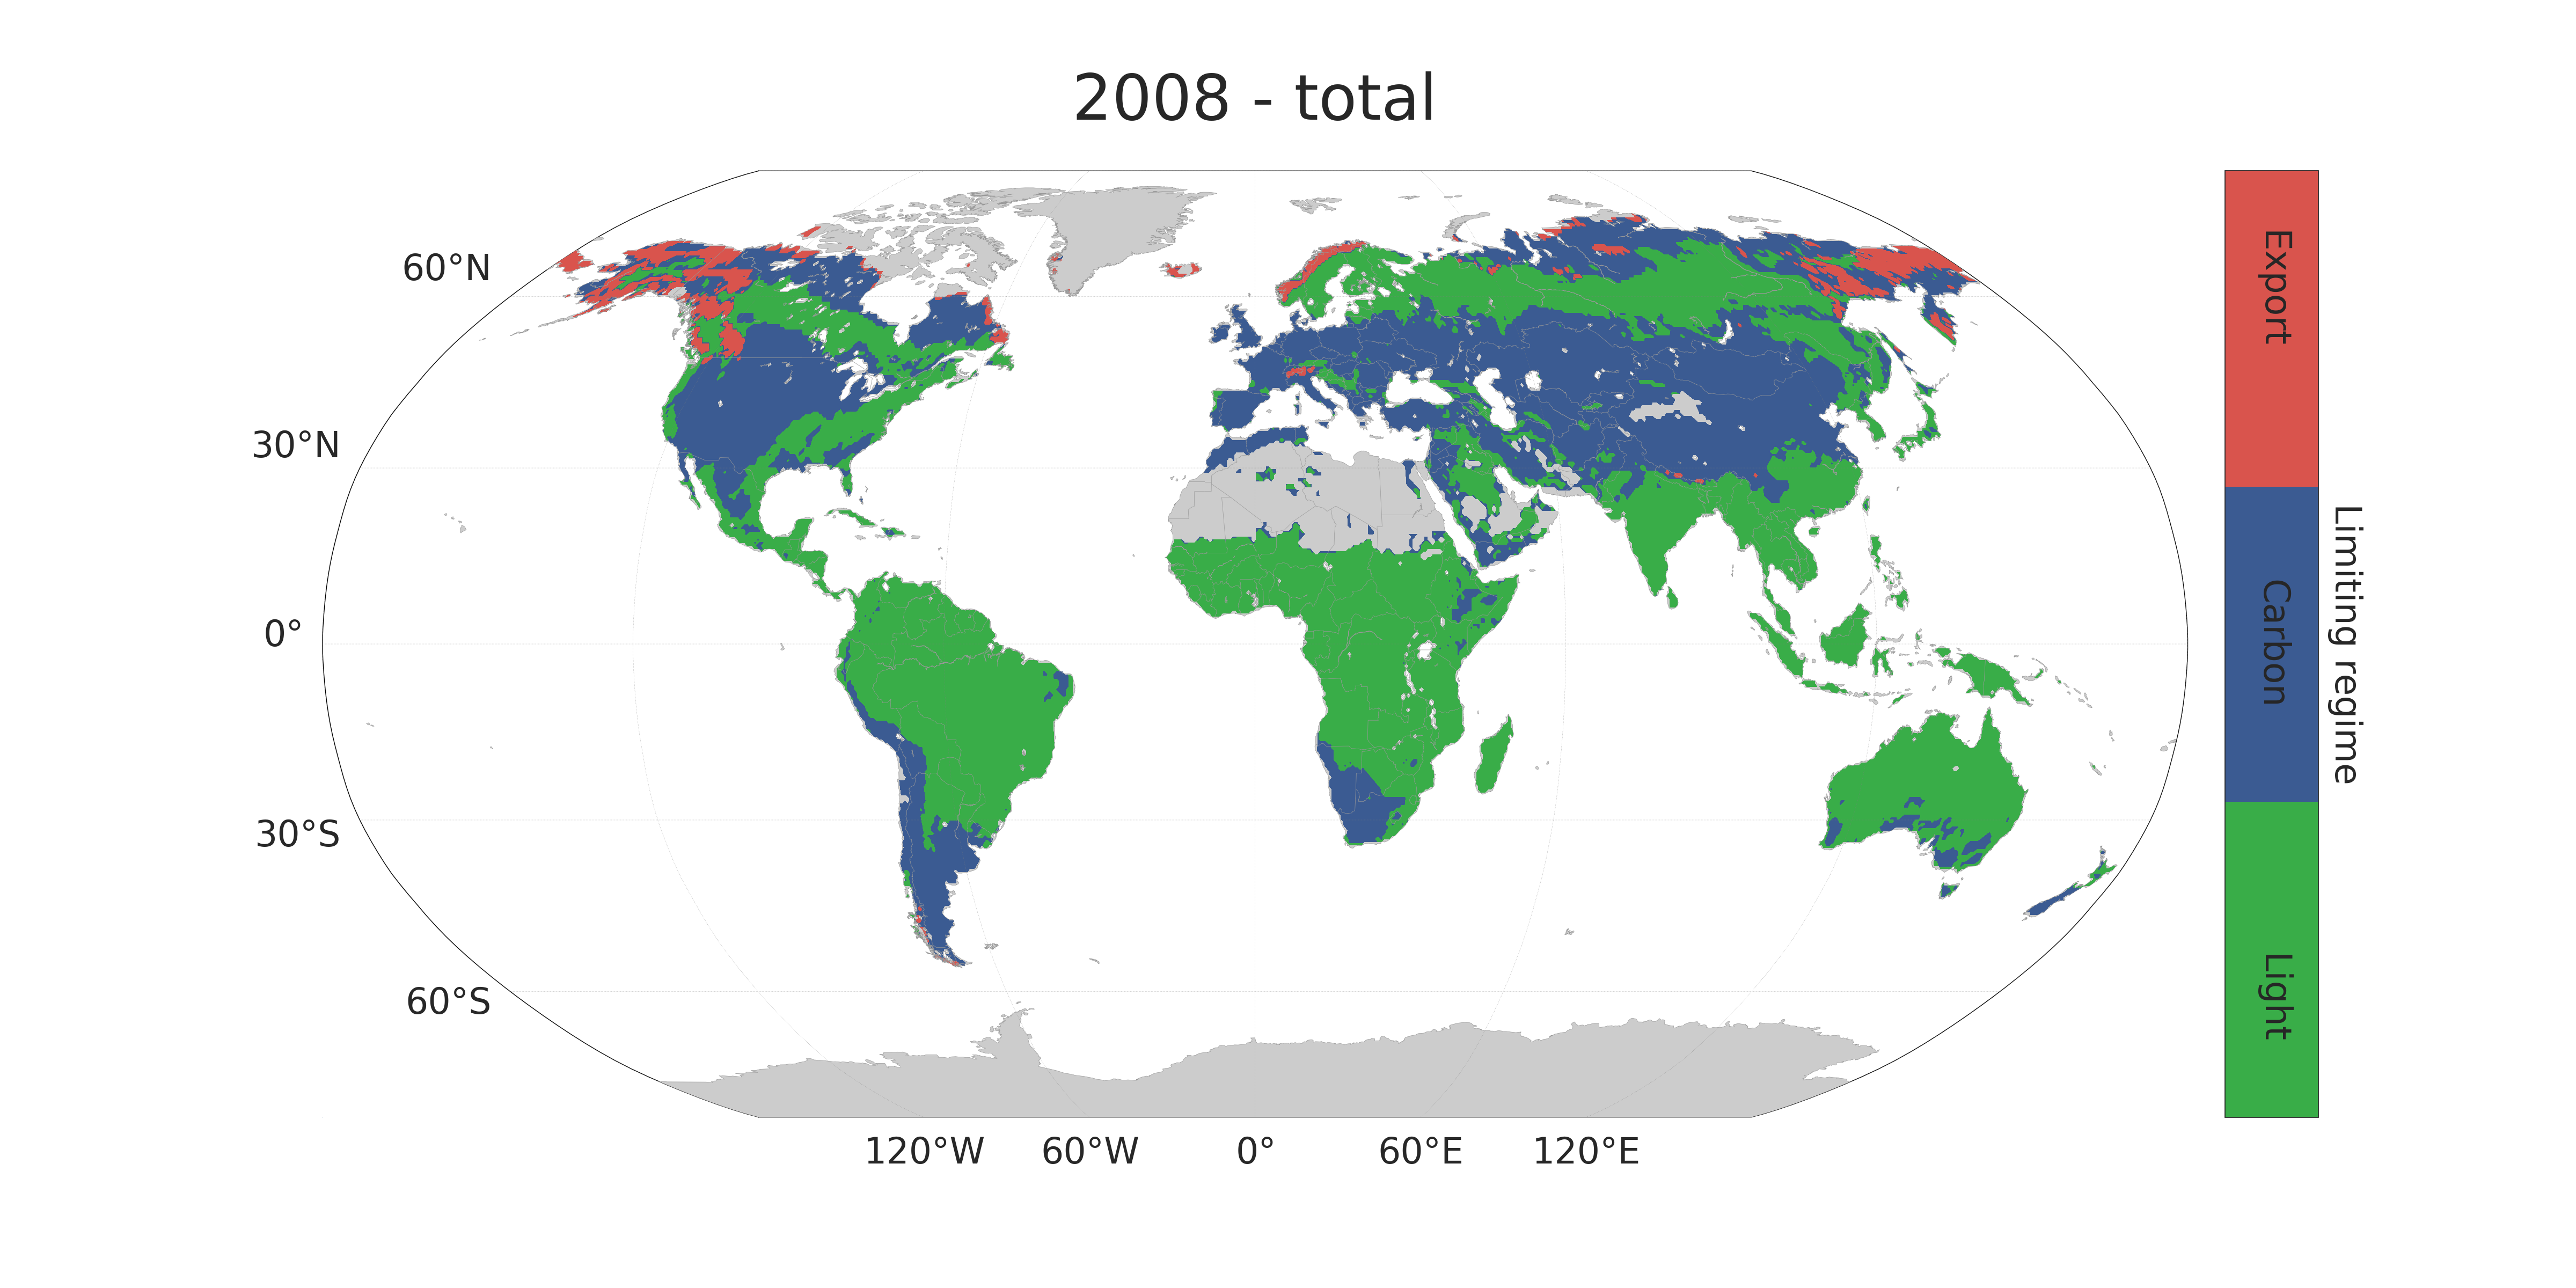
\includegraphics[width=0.33\textwidth]{/home/mn811042/Thesis/chapter6/figures_ofi/Farquhar_year_total_opt5_integral.png}}
\subfloat[Opt 5 clump]{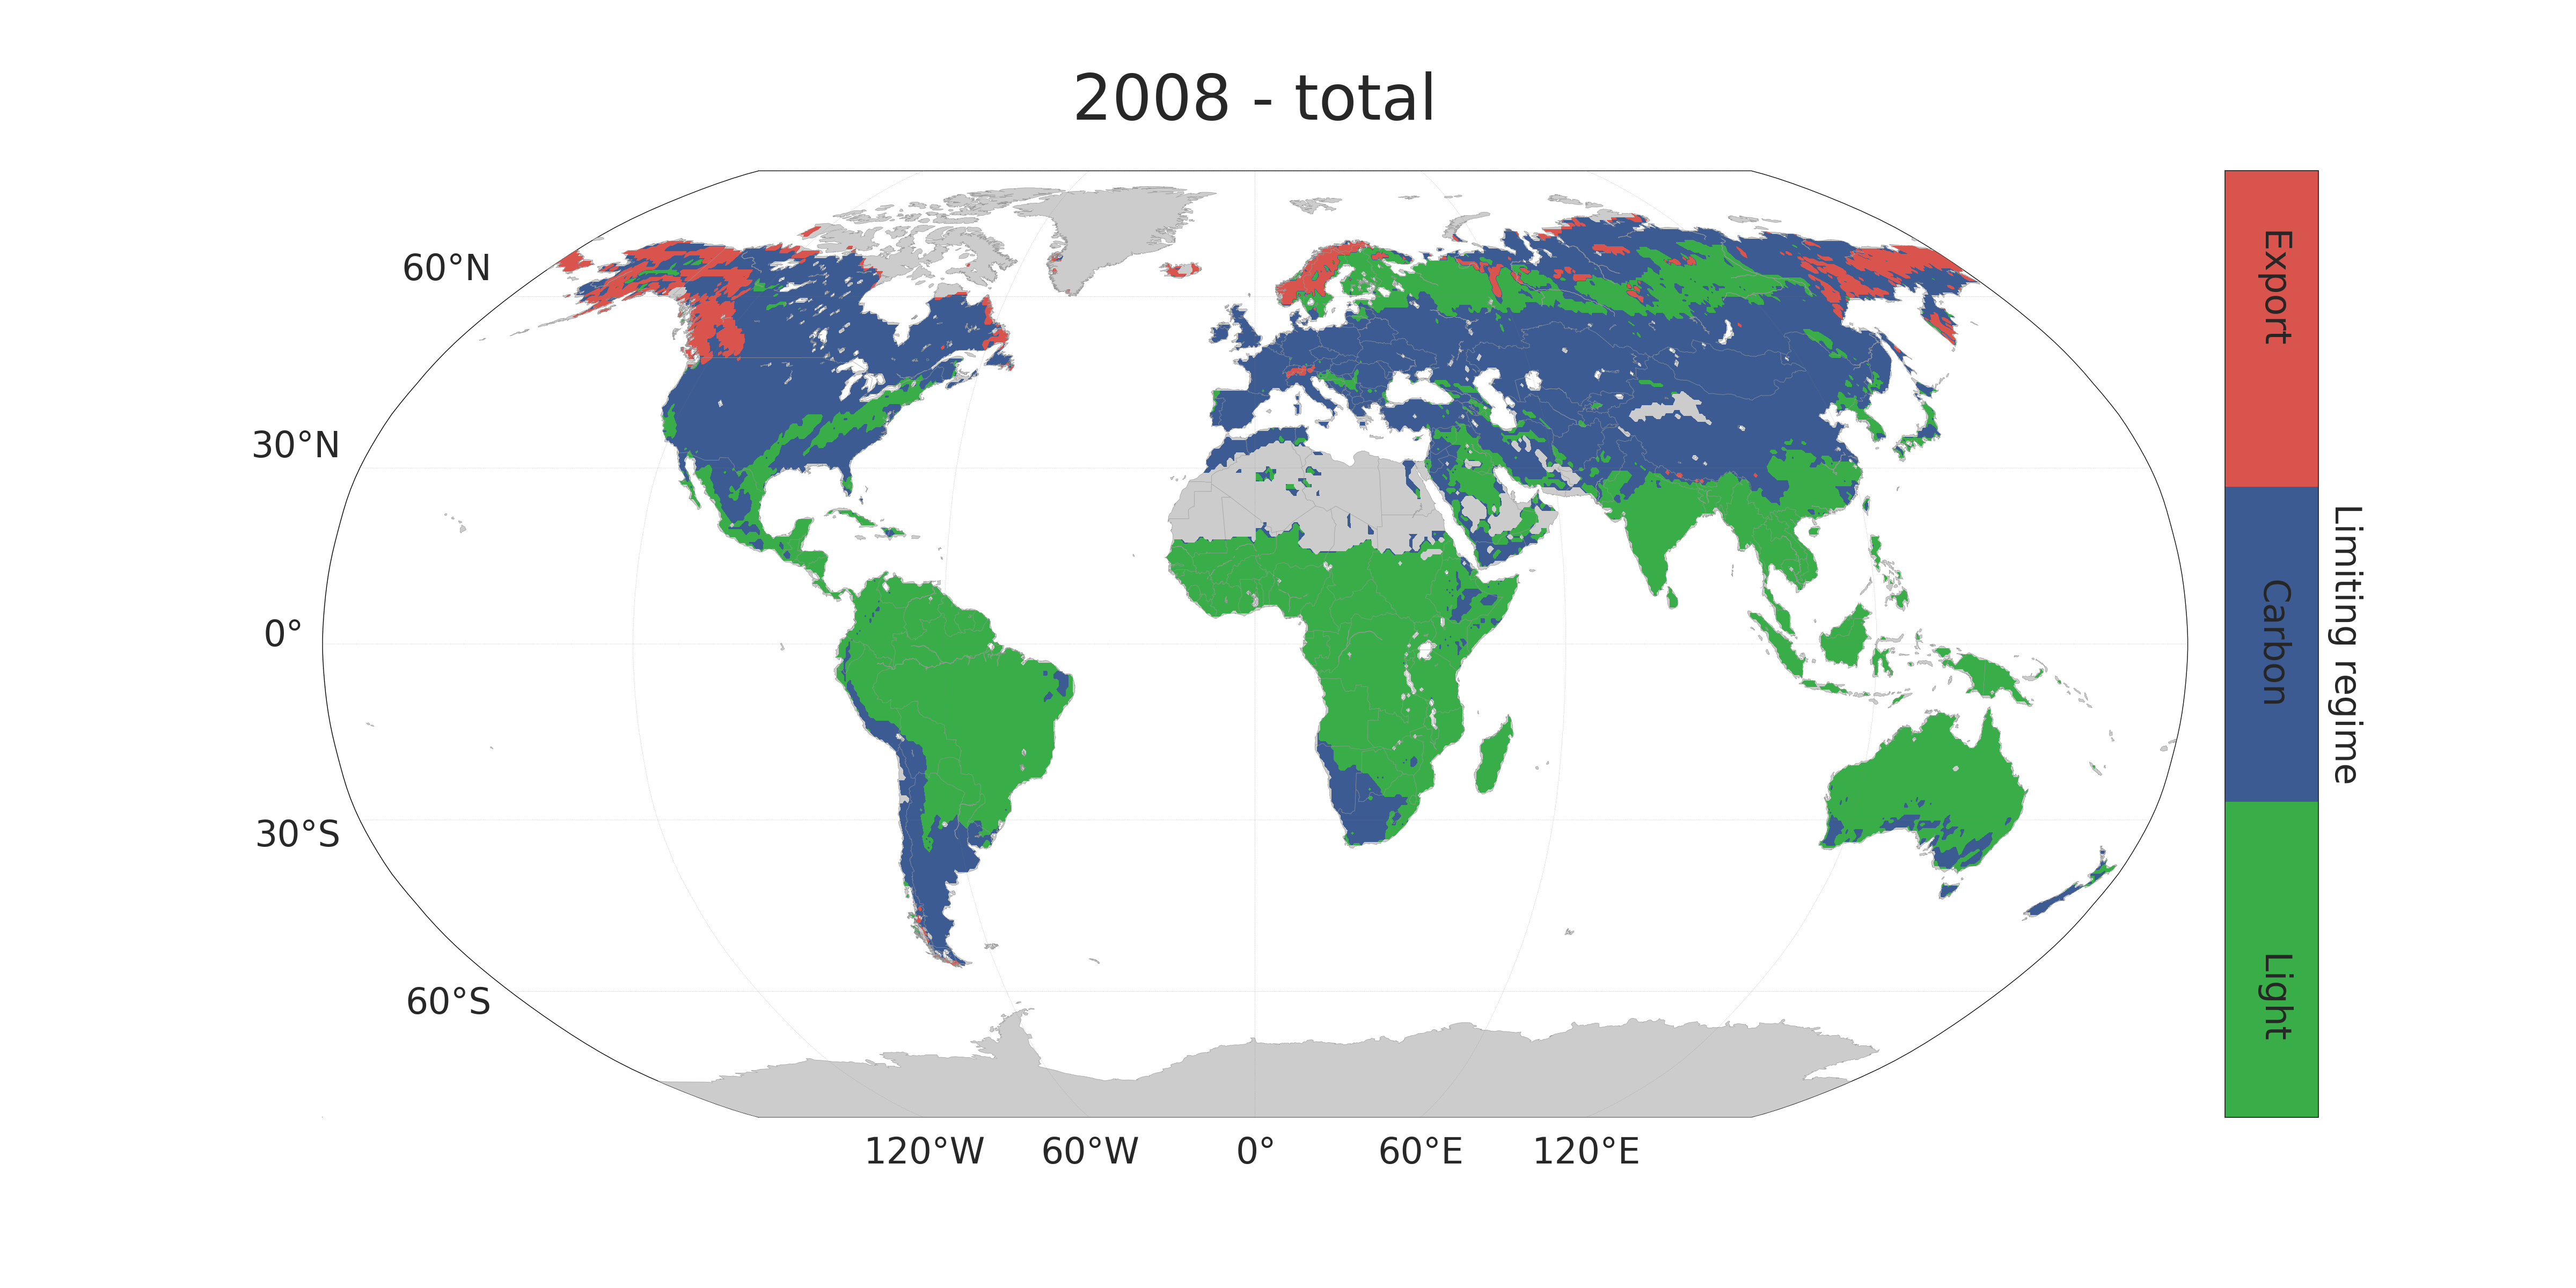
\includegraphics[width=0.33\textwidth]{/home/mn811042/Thesis/chapter6/figures_ofi/Farquhar_year_total_opt5_clump_integral.png}}
\subfloat[Difference]{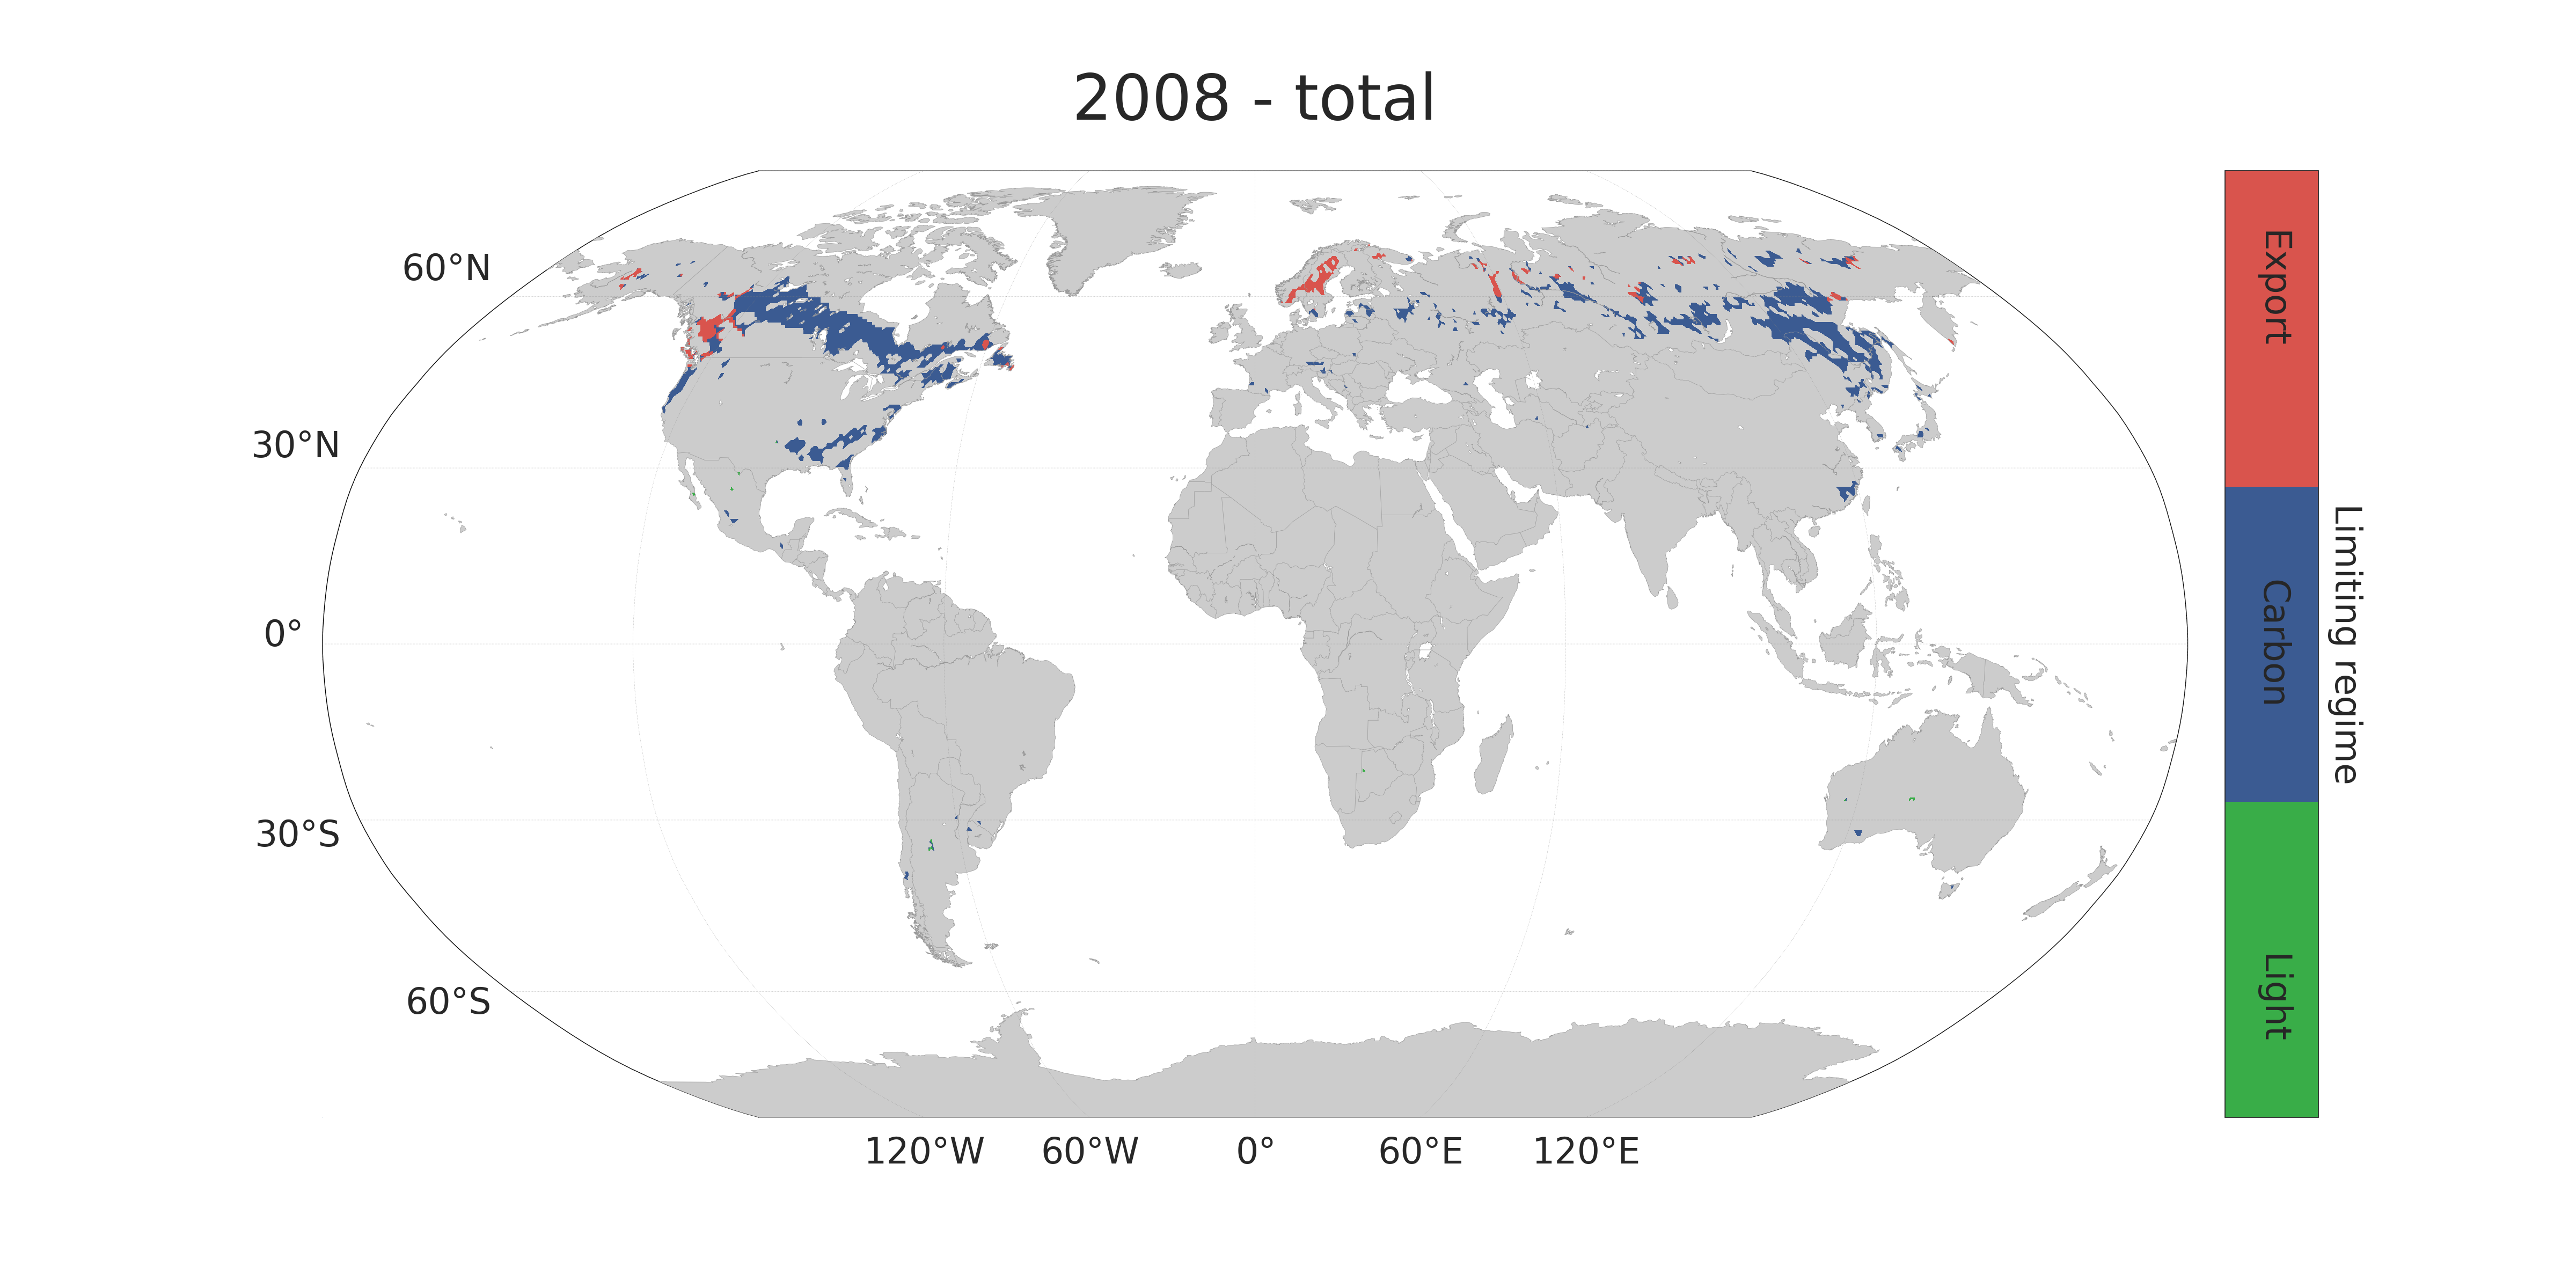
\includegraphics[width=0.33\textwidth]{/home/mn811042/Thesis/chapter6/figures_ofi/Farquhar_year_total_opt5_clump_integral_diff.png}}
\end{tabular}
\begin{tabular}{lll}
\subfloat[Opt 5]{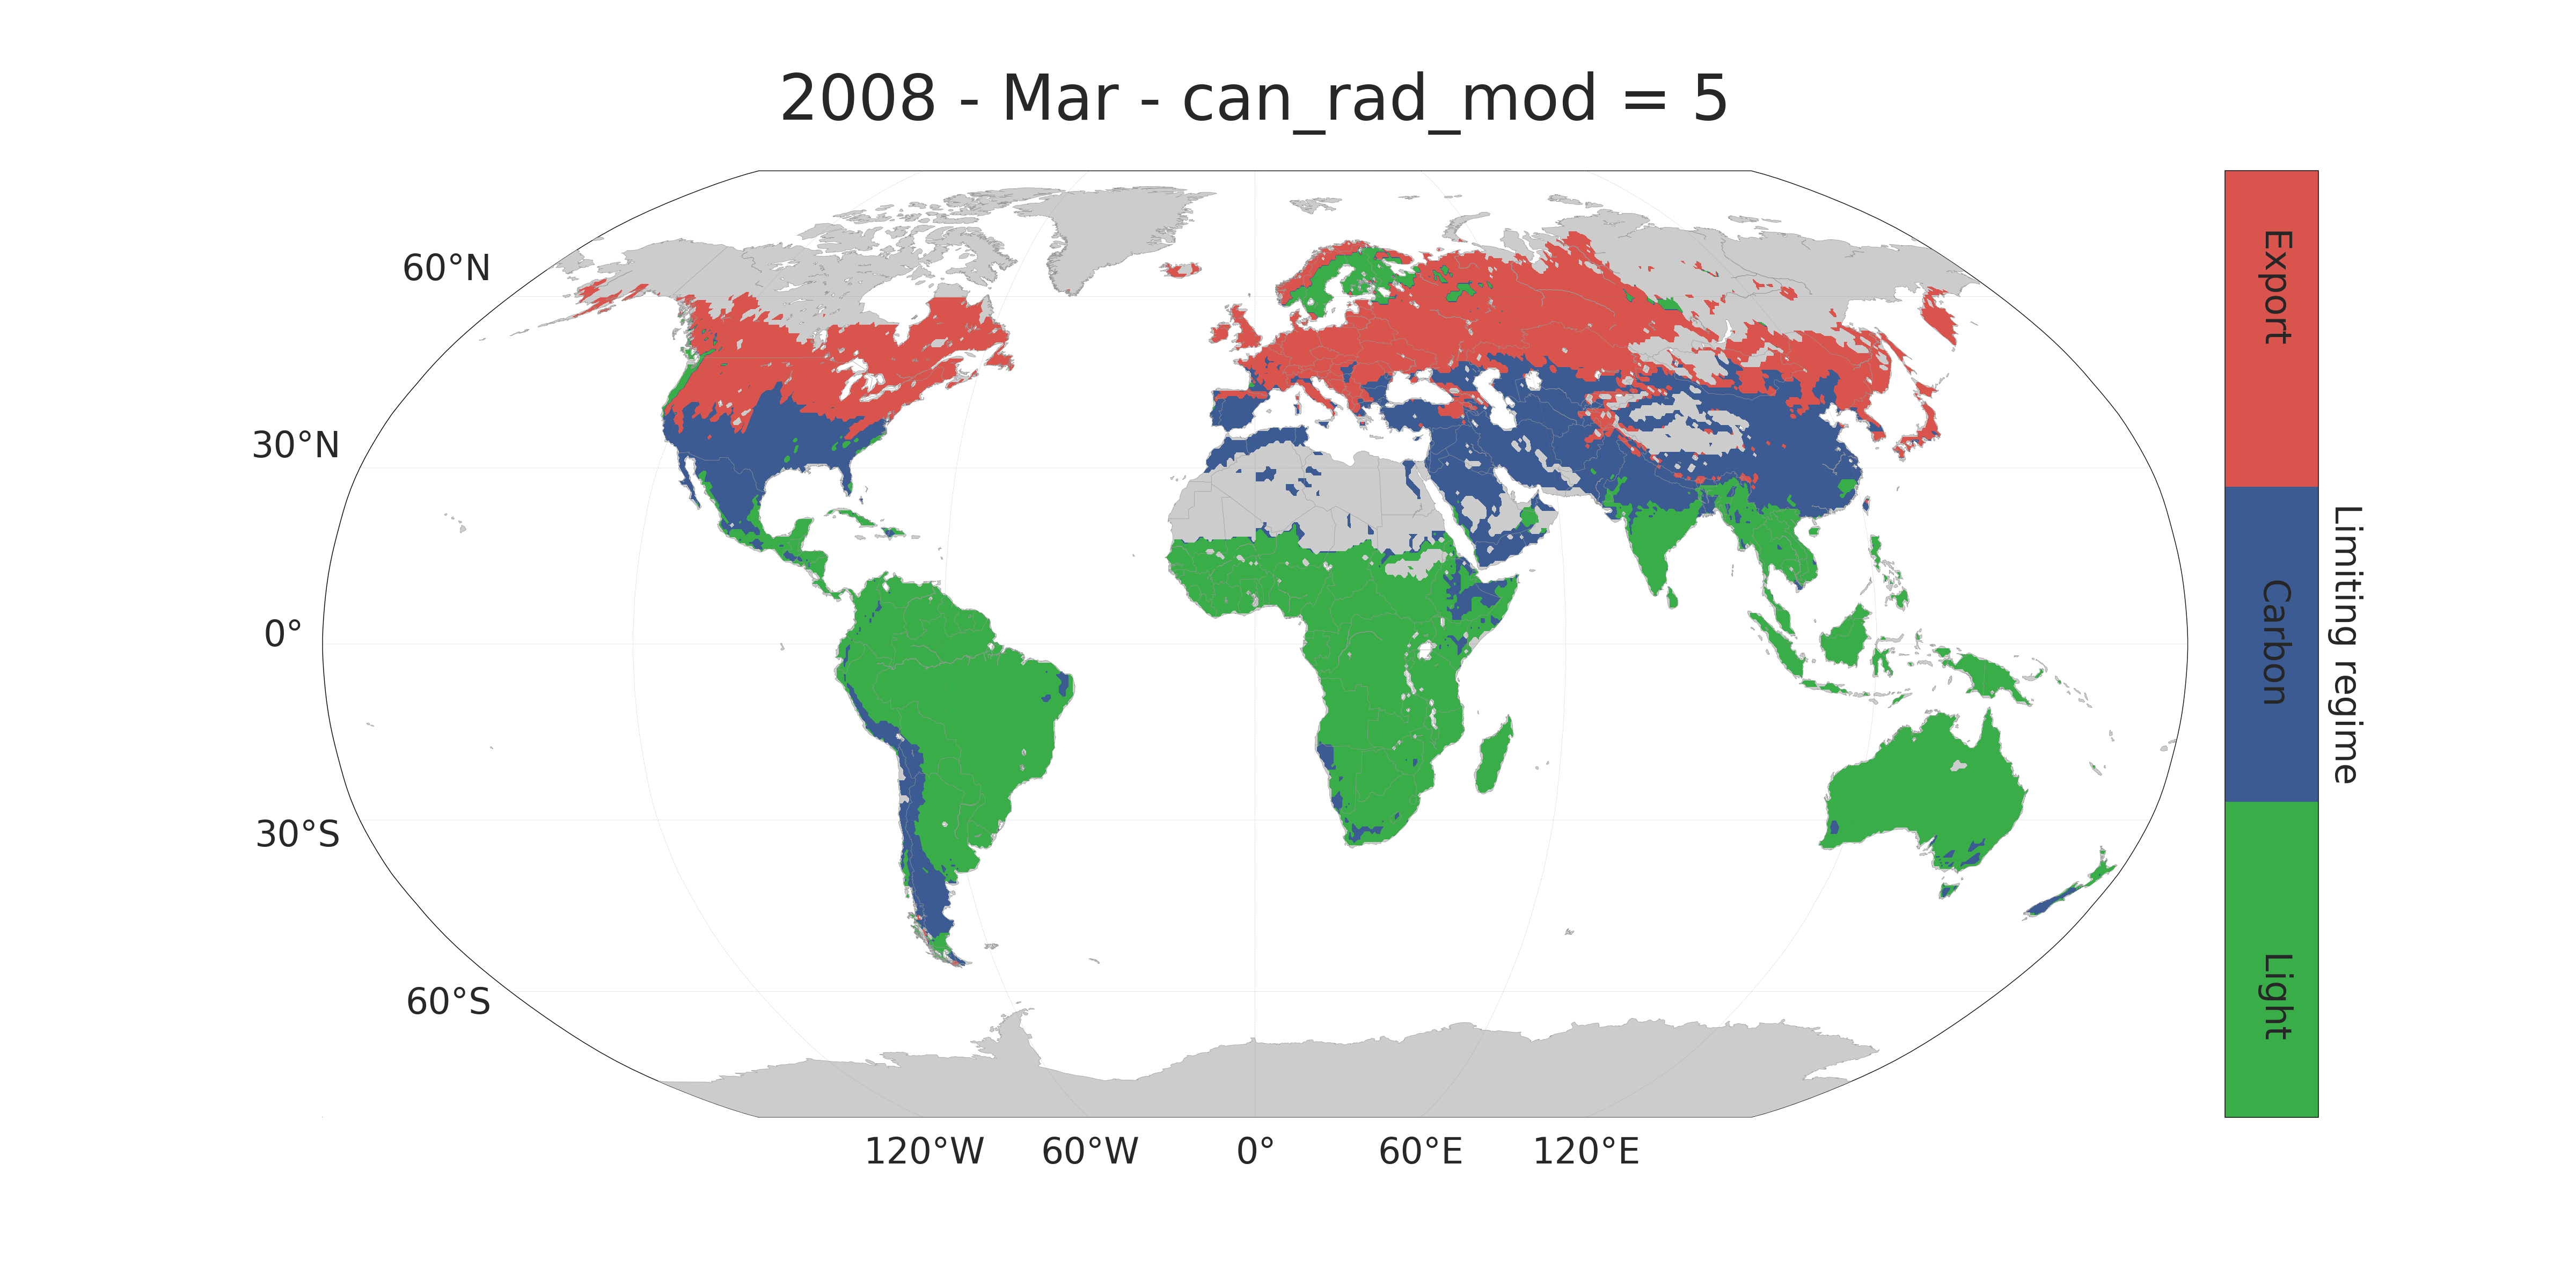
\includegraphics[width=0.33\textwidth]{/home/mn811042/Thesis/chapter6/figures_ofi/Farquhar_opt5_Mar_integral.png}}
\subfloat[Opt 5 clump]{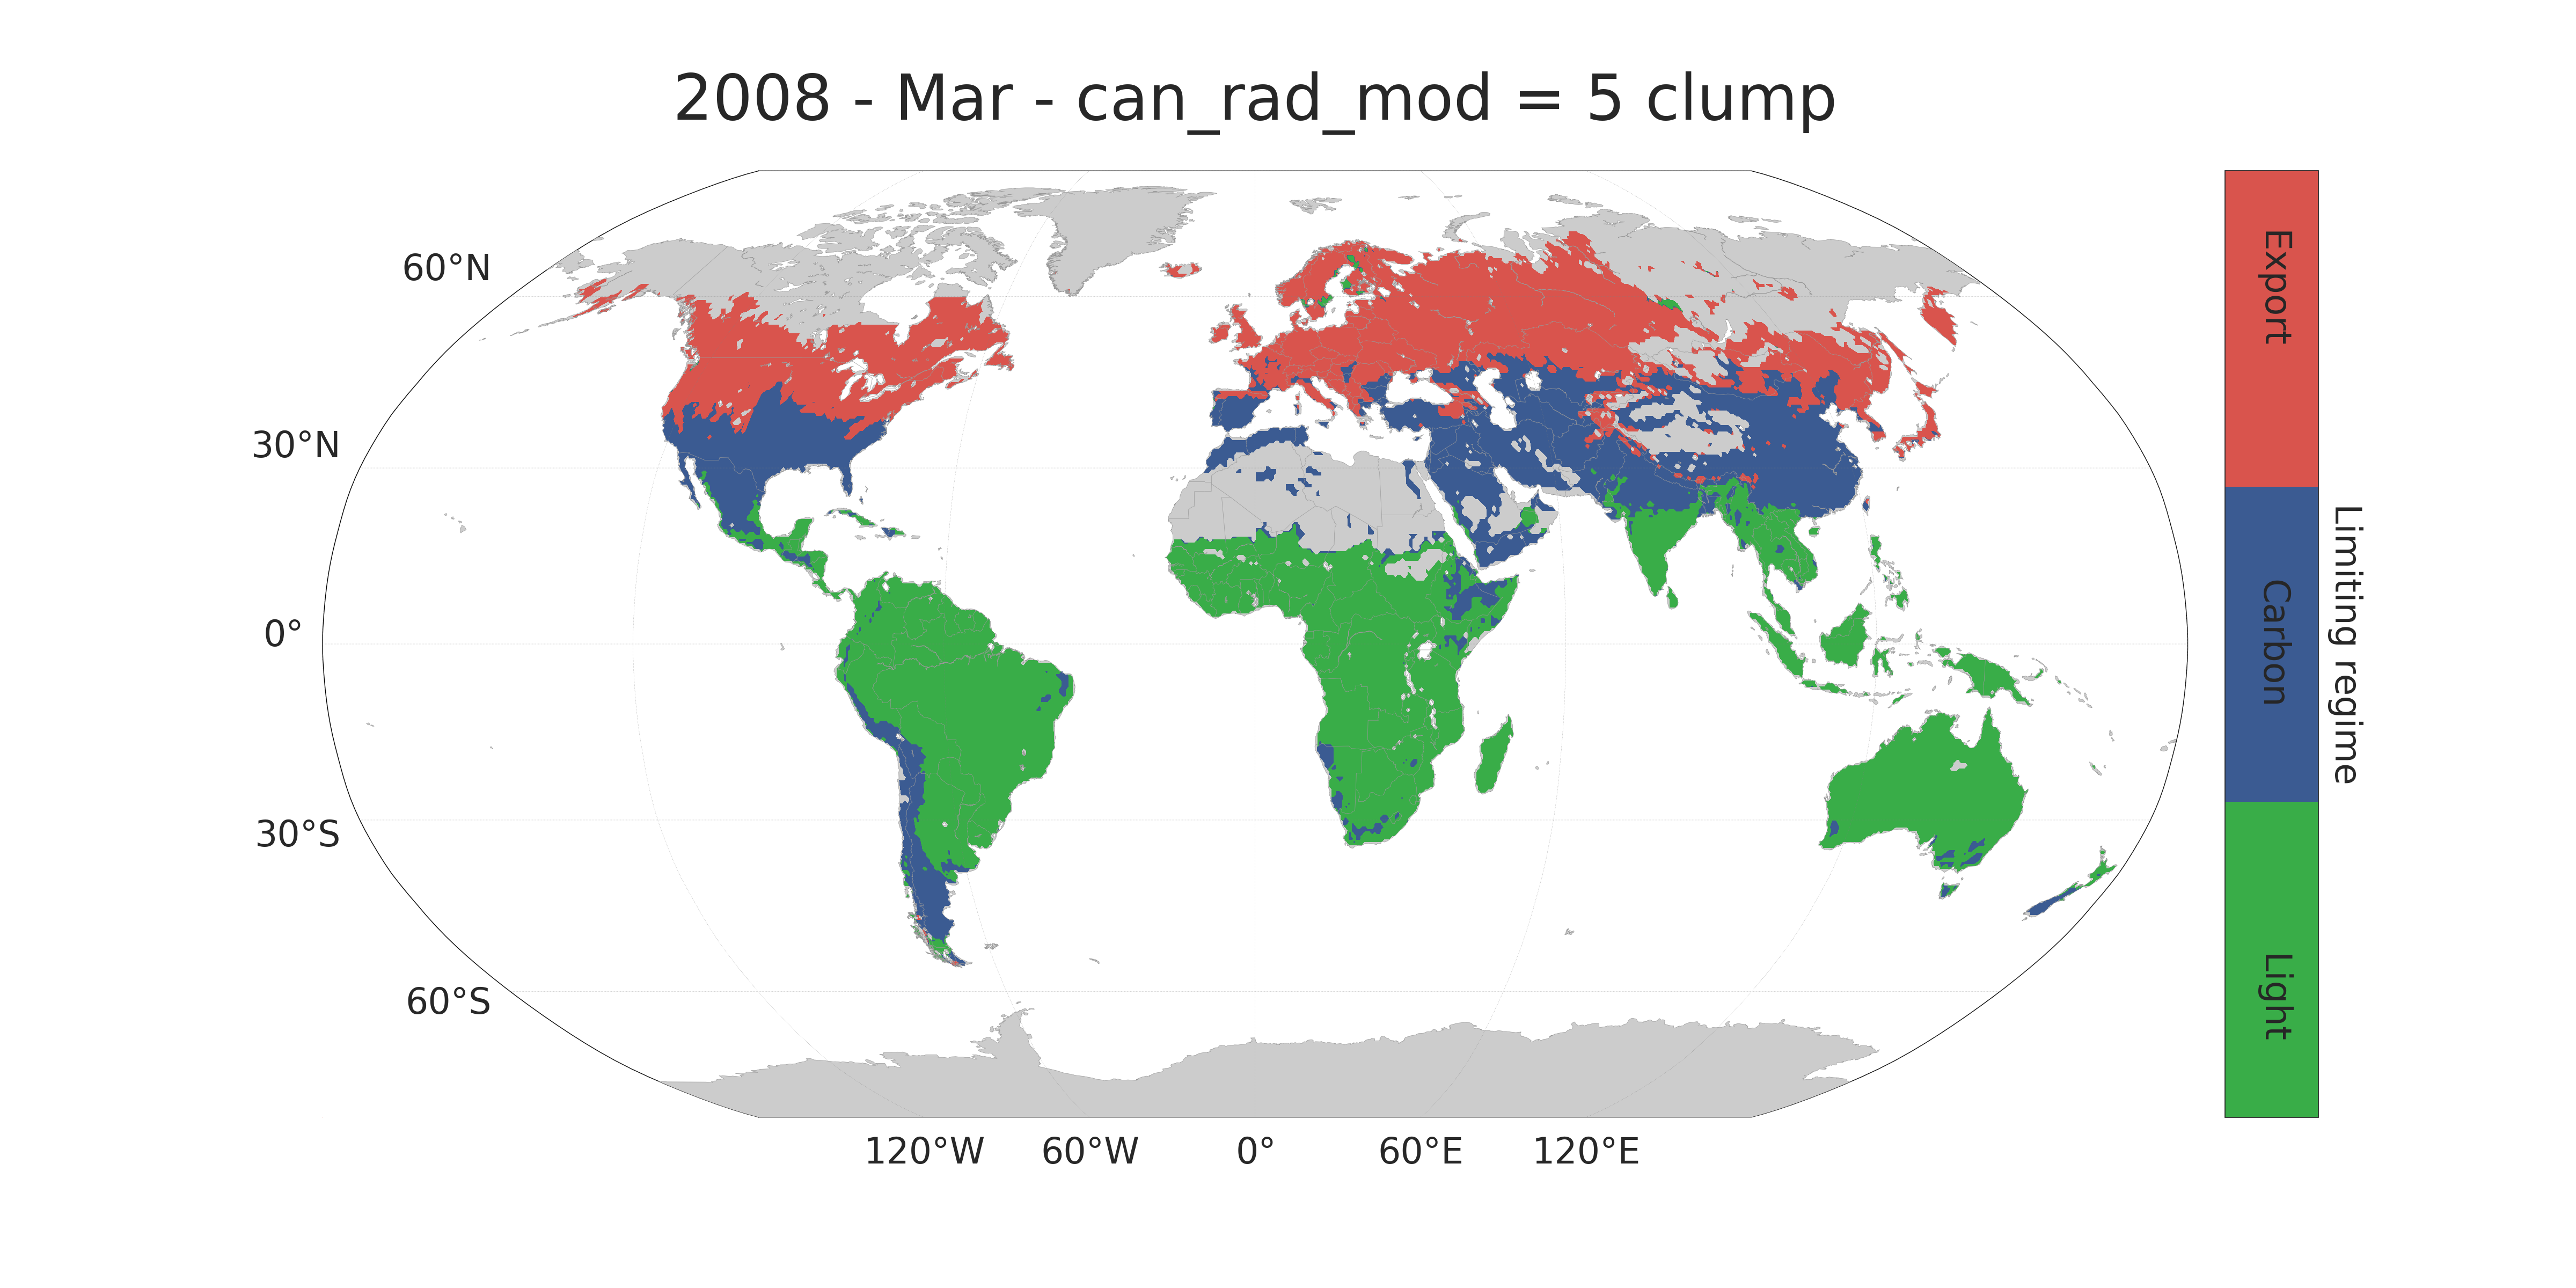
\includegraphics[width=0.33\textwidth]{/home/mn811042/Thesis/chapter6/figures_ofi/Farquhar_opt5_clump_Mar_integral.png}}
\subfloat[Difference]{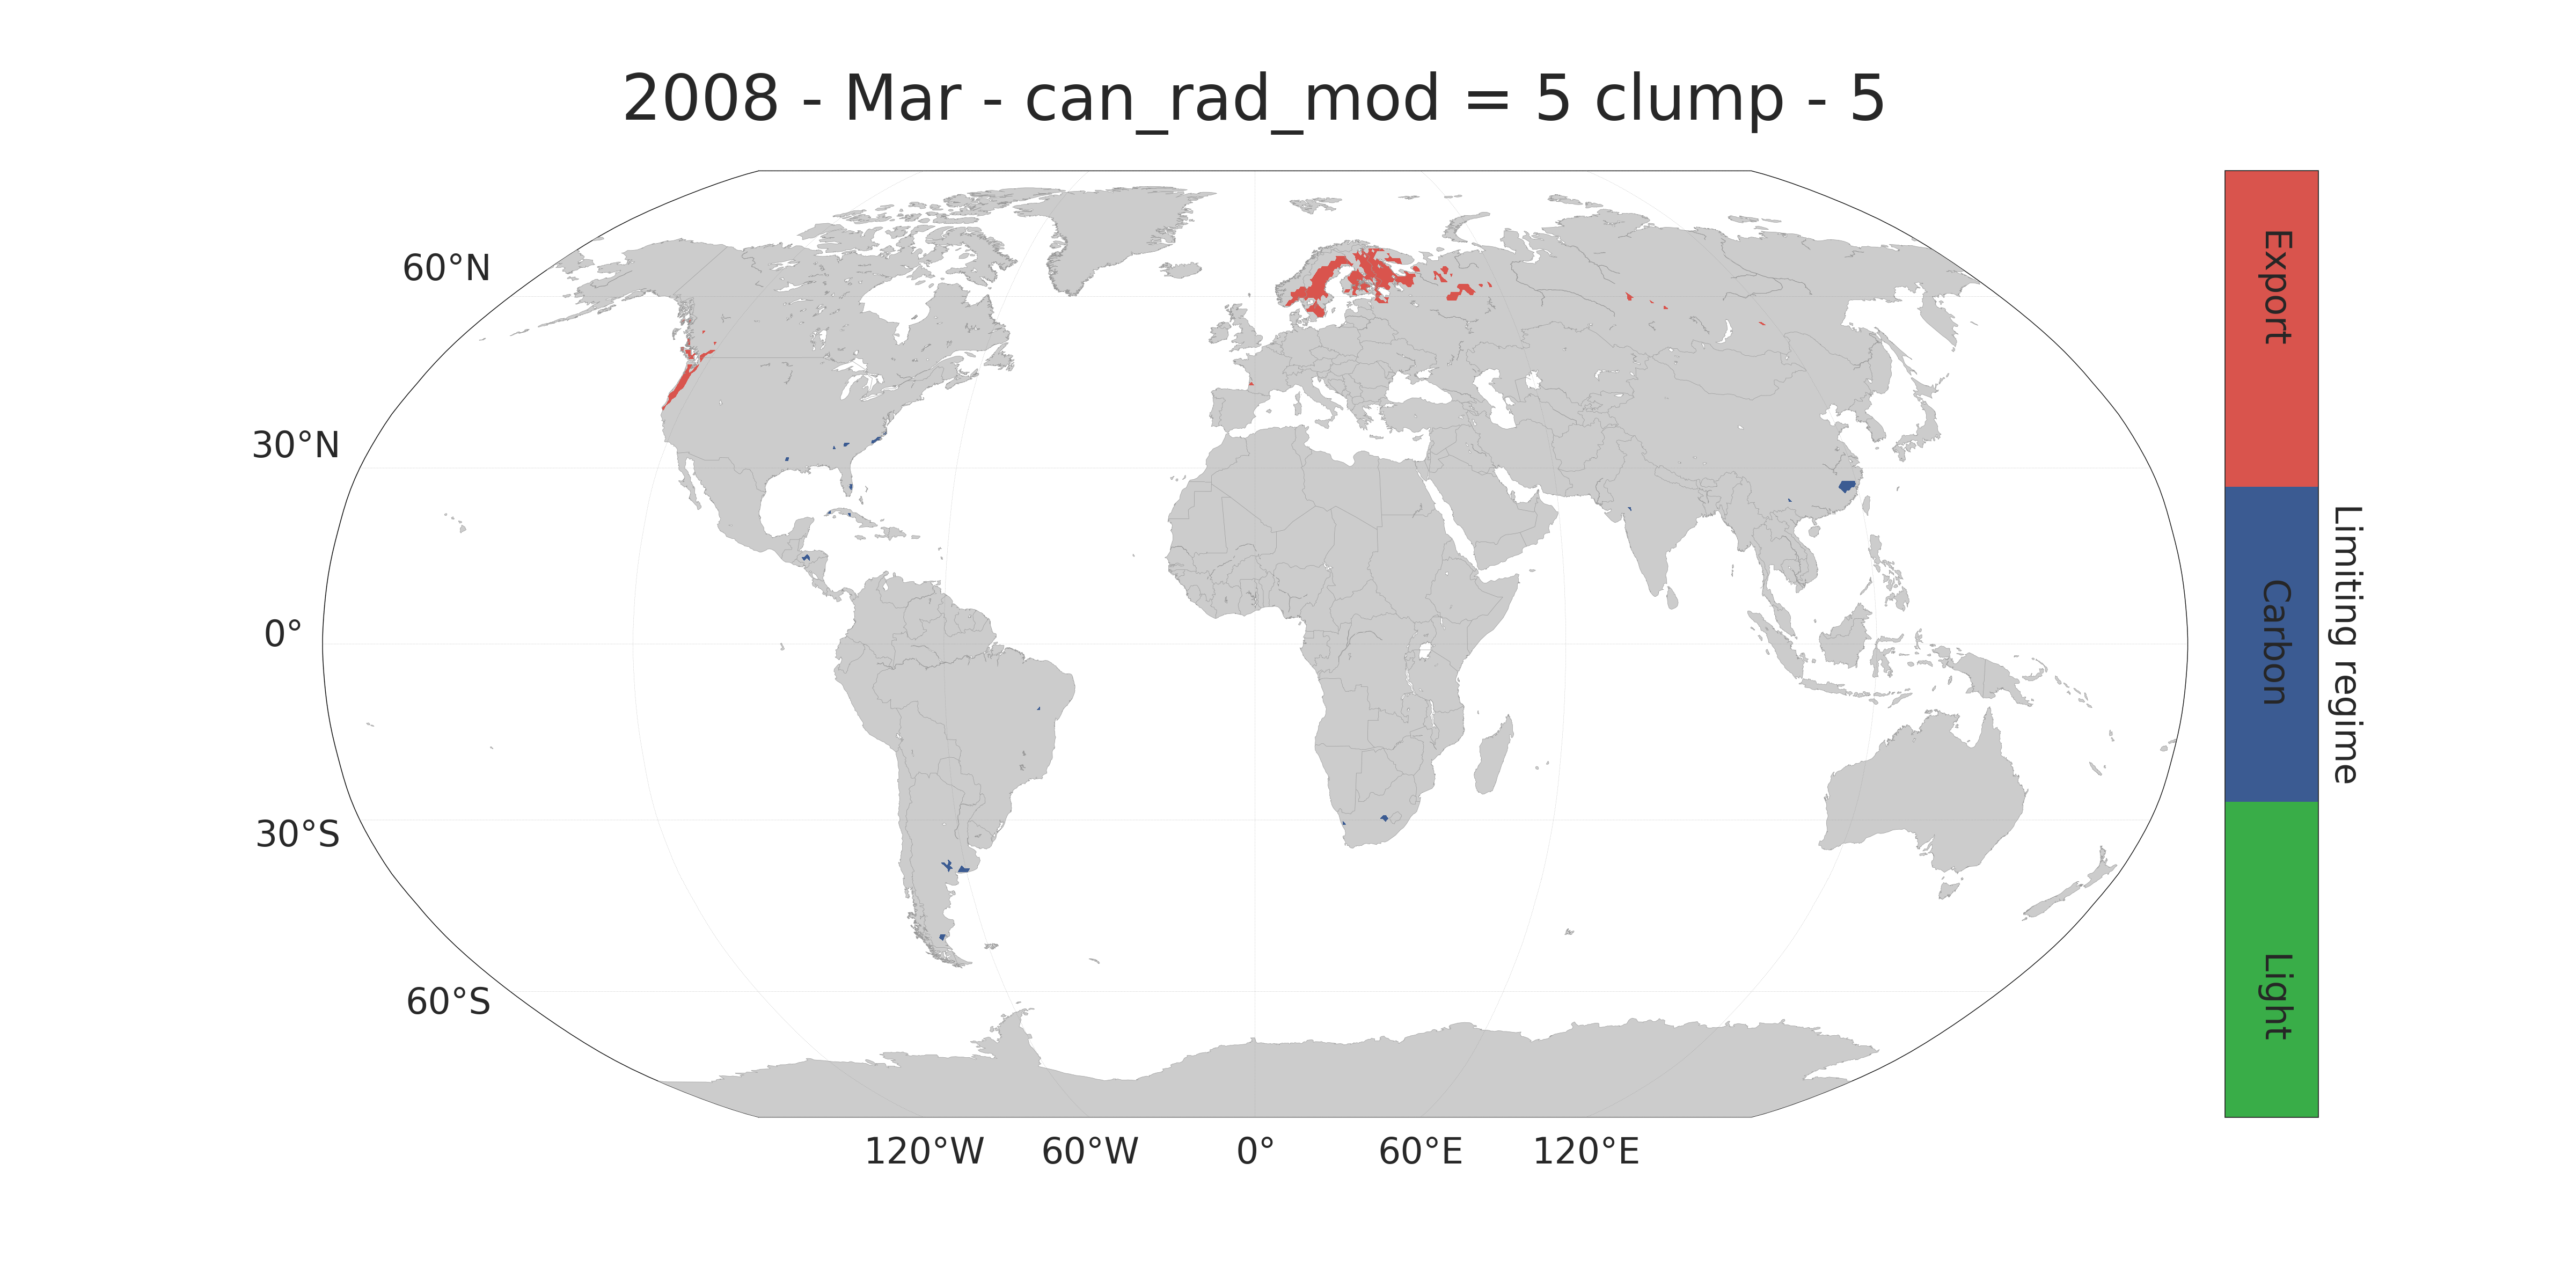
\includegraphics[width=0.33\textwidth]{/home/mn811042/Thesis/chapter6/figures_ofi/Farquhar_opt5_anomaly_Mar_integral.png}}
\end{tabular}
\begin{tabular}{lll}
\subfloat[Opt 5]{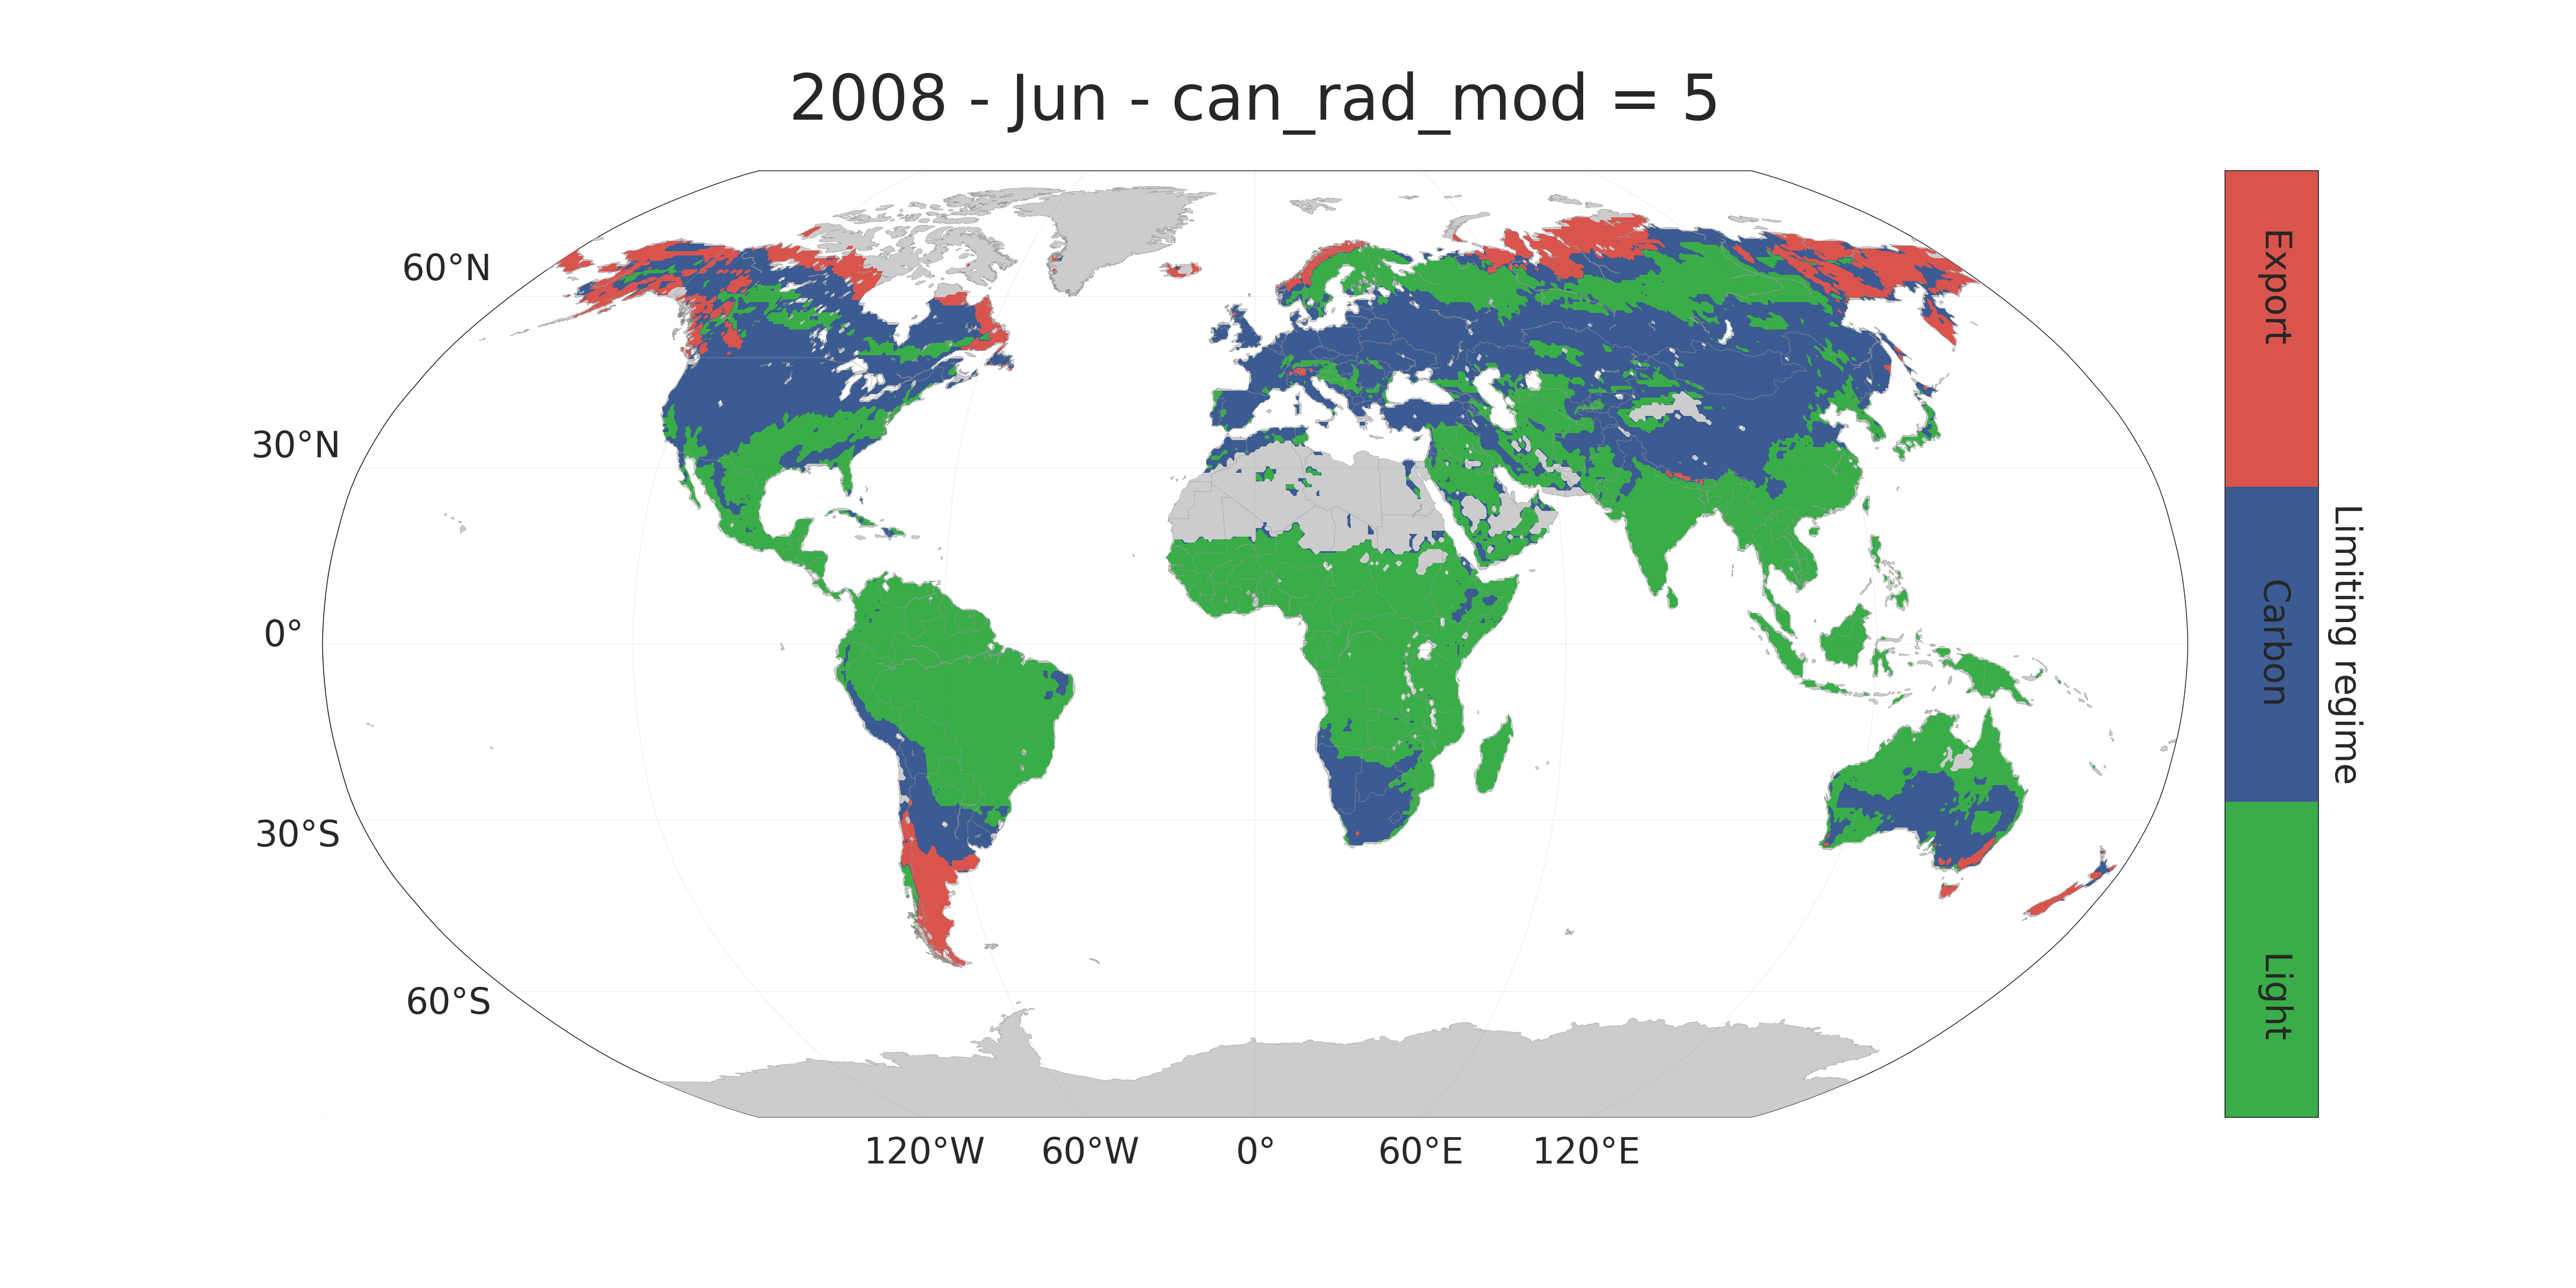
\includegraphics[width=0.33\textwidth]{/home/mn811042/Thesis/chapter6/figures_ofi/Farquhar_opt5_Jun_integral.png}}
\subfloat[Opt 5 clump]{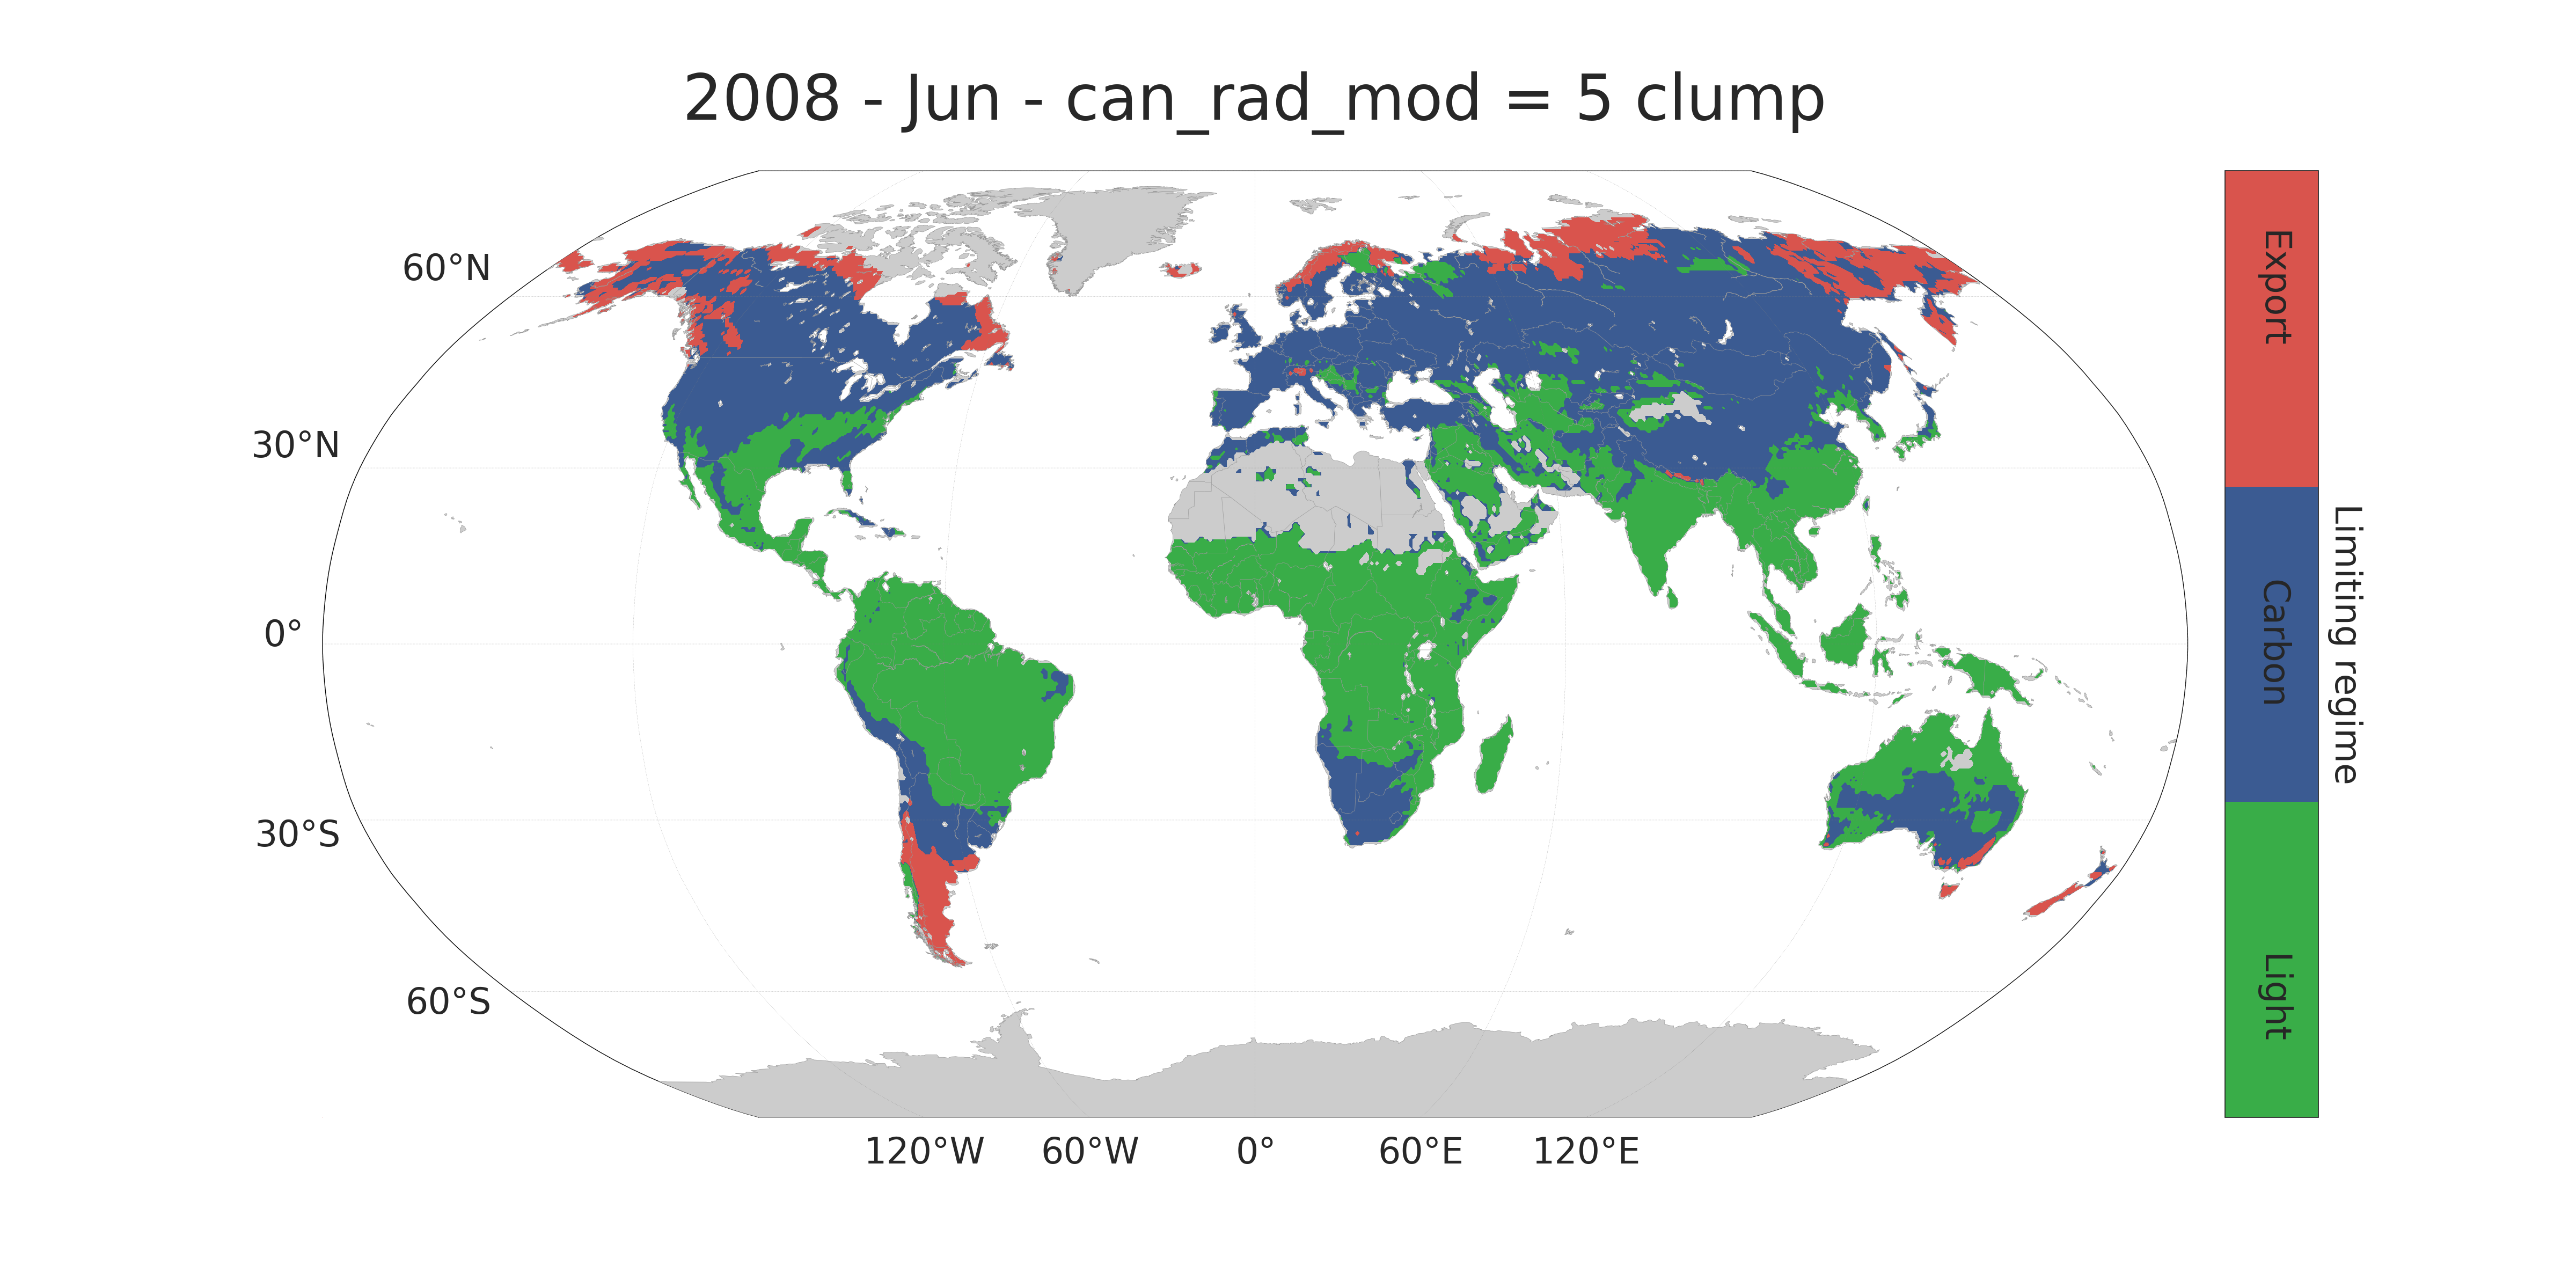
\includegraphics[width=0.33\textwidth]{/home/mn811042/Thesis/chapter6/figures_ofi/Farquhar_opt5_clump_Jun_integral.png}}
\subfloat[Difference]{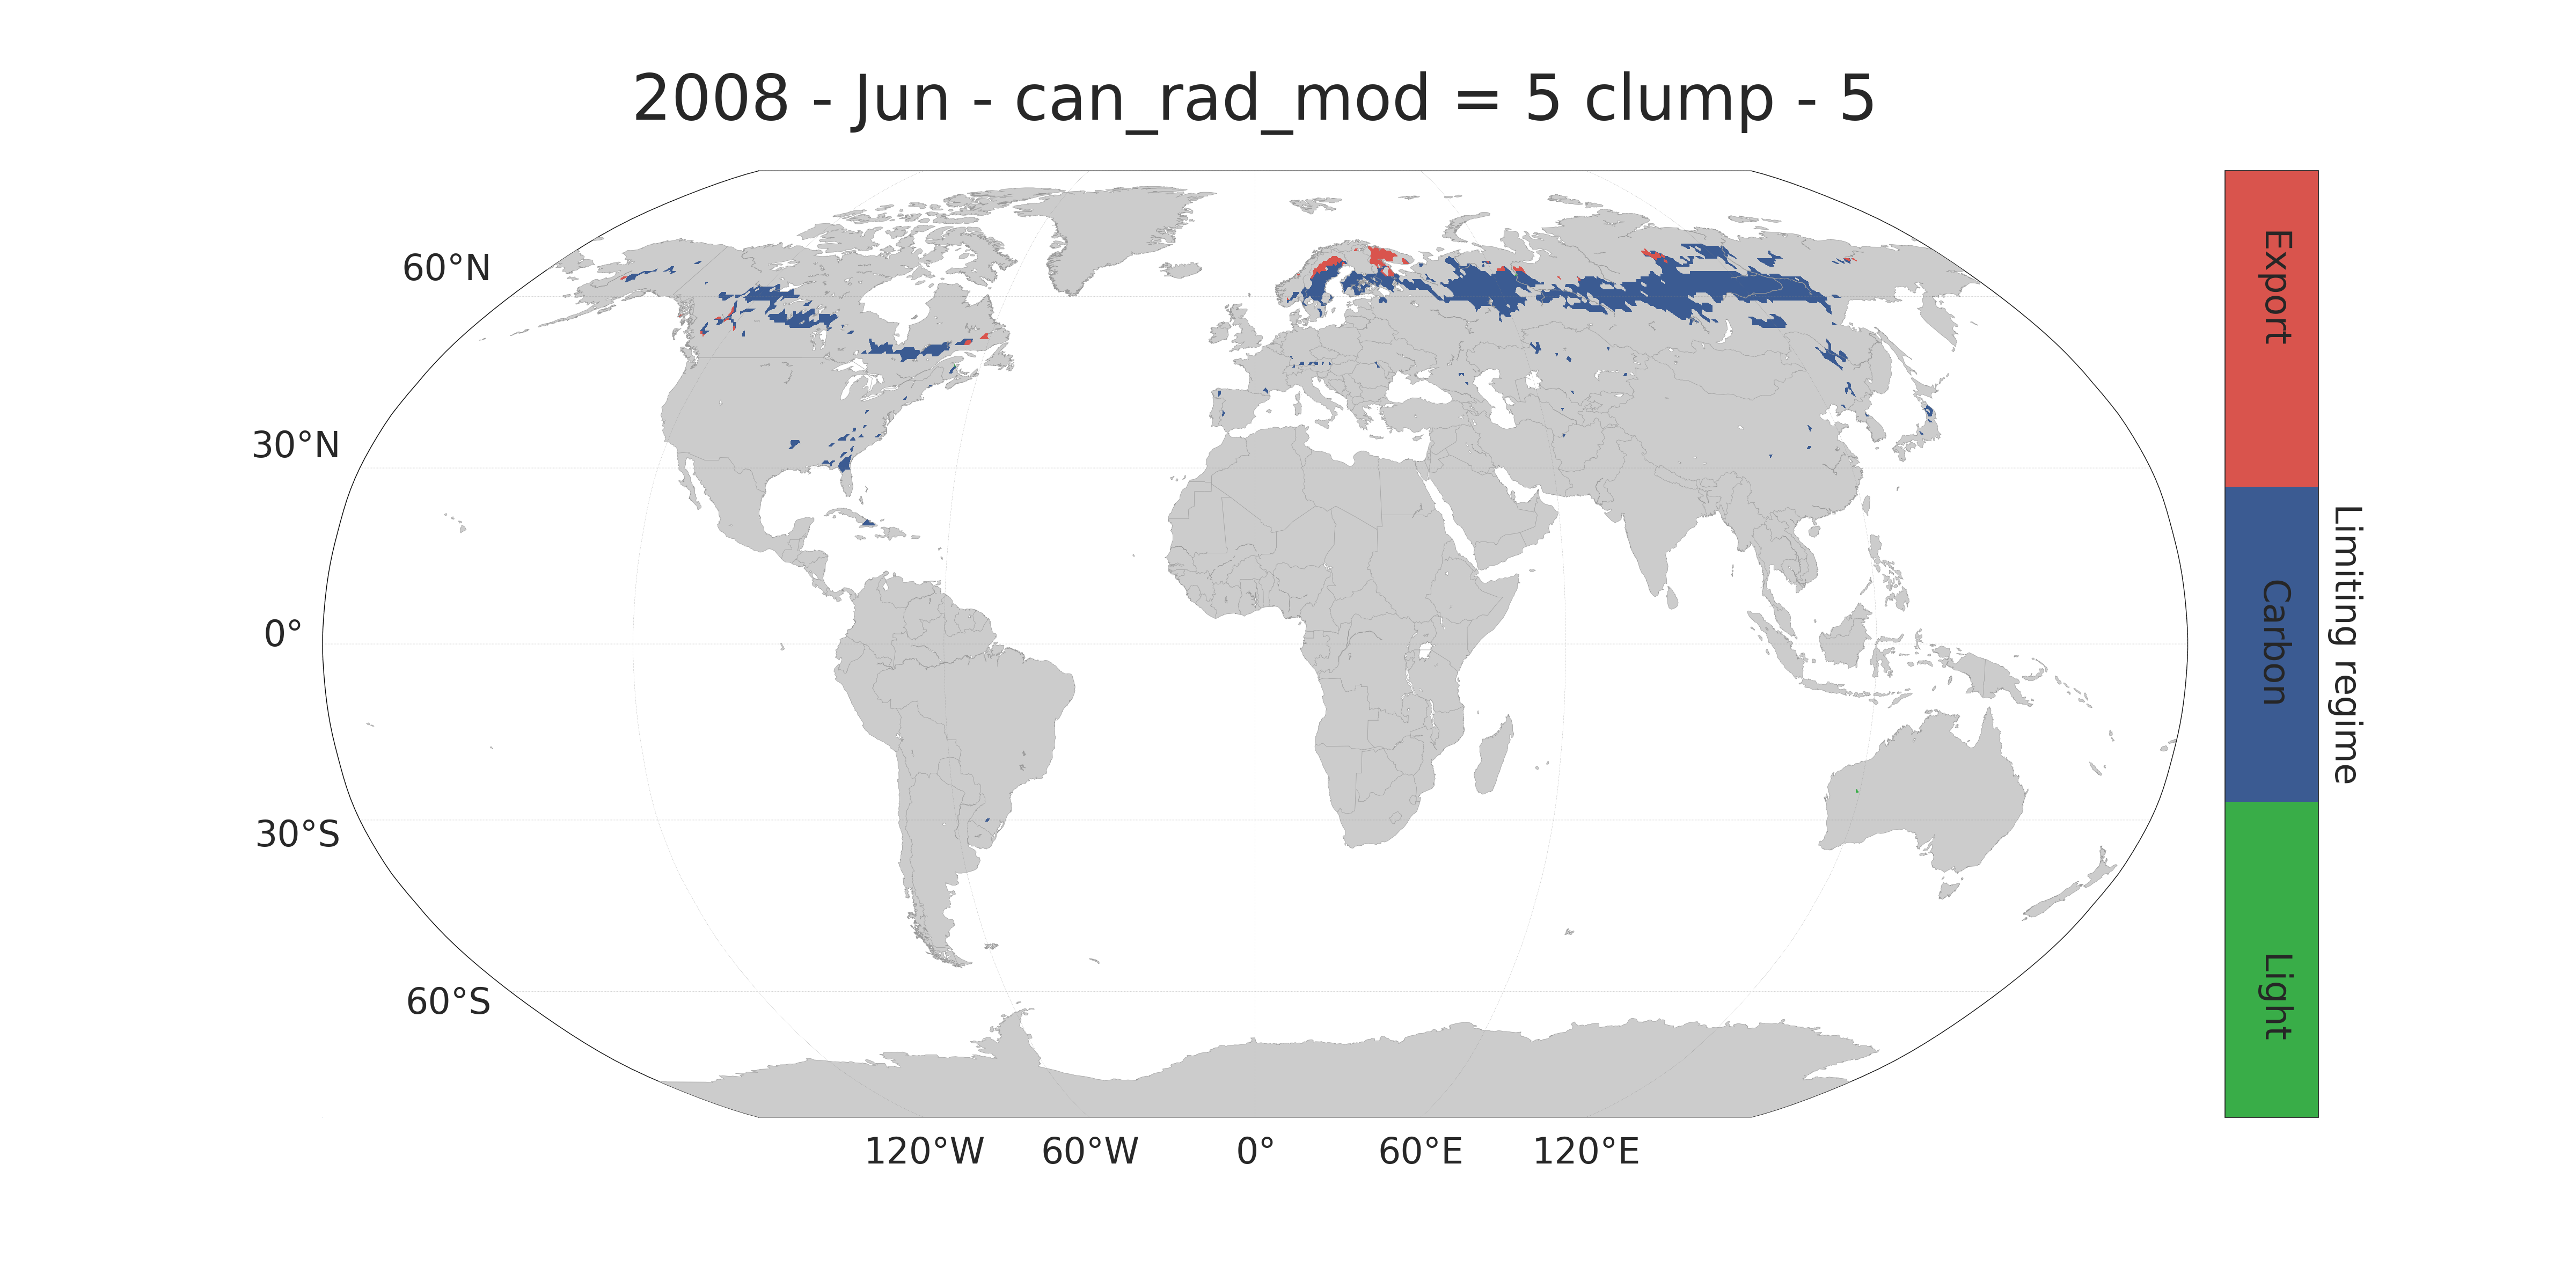
\includegraphics[width=0.33\textwidth]{/home/mn811042/Thesis/chapter6/figures_ofi/Farquhar_opt5_anomaly_Jun_integral.png}}
\end{tabular}
\begin{tabular}{lll}
\subfloat[Opt 5]{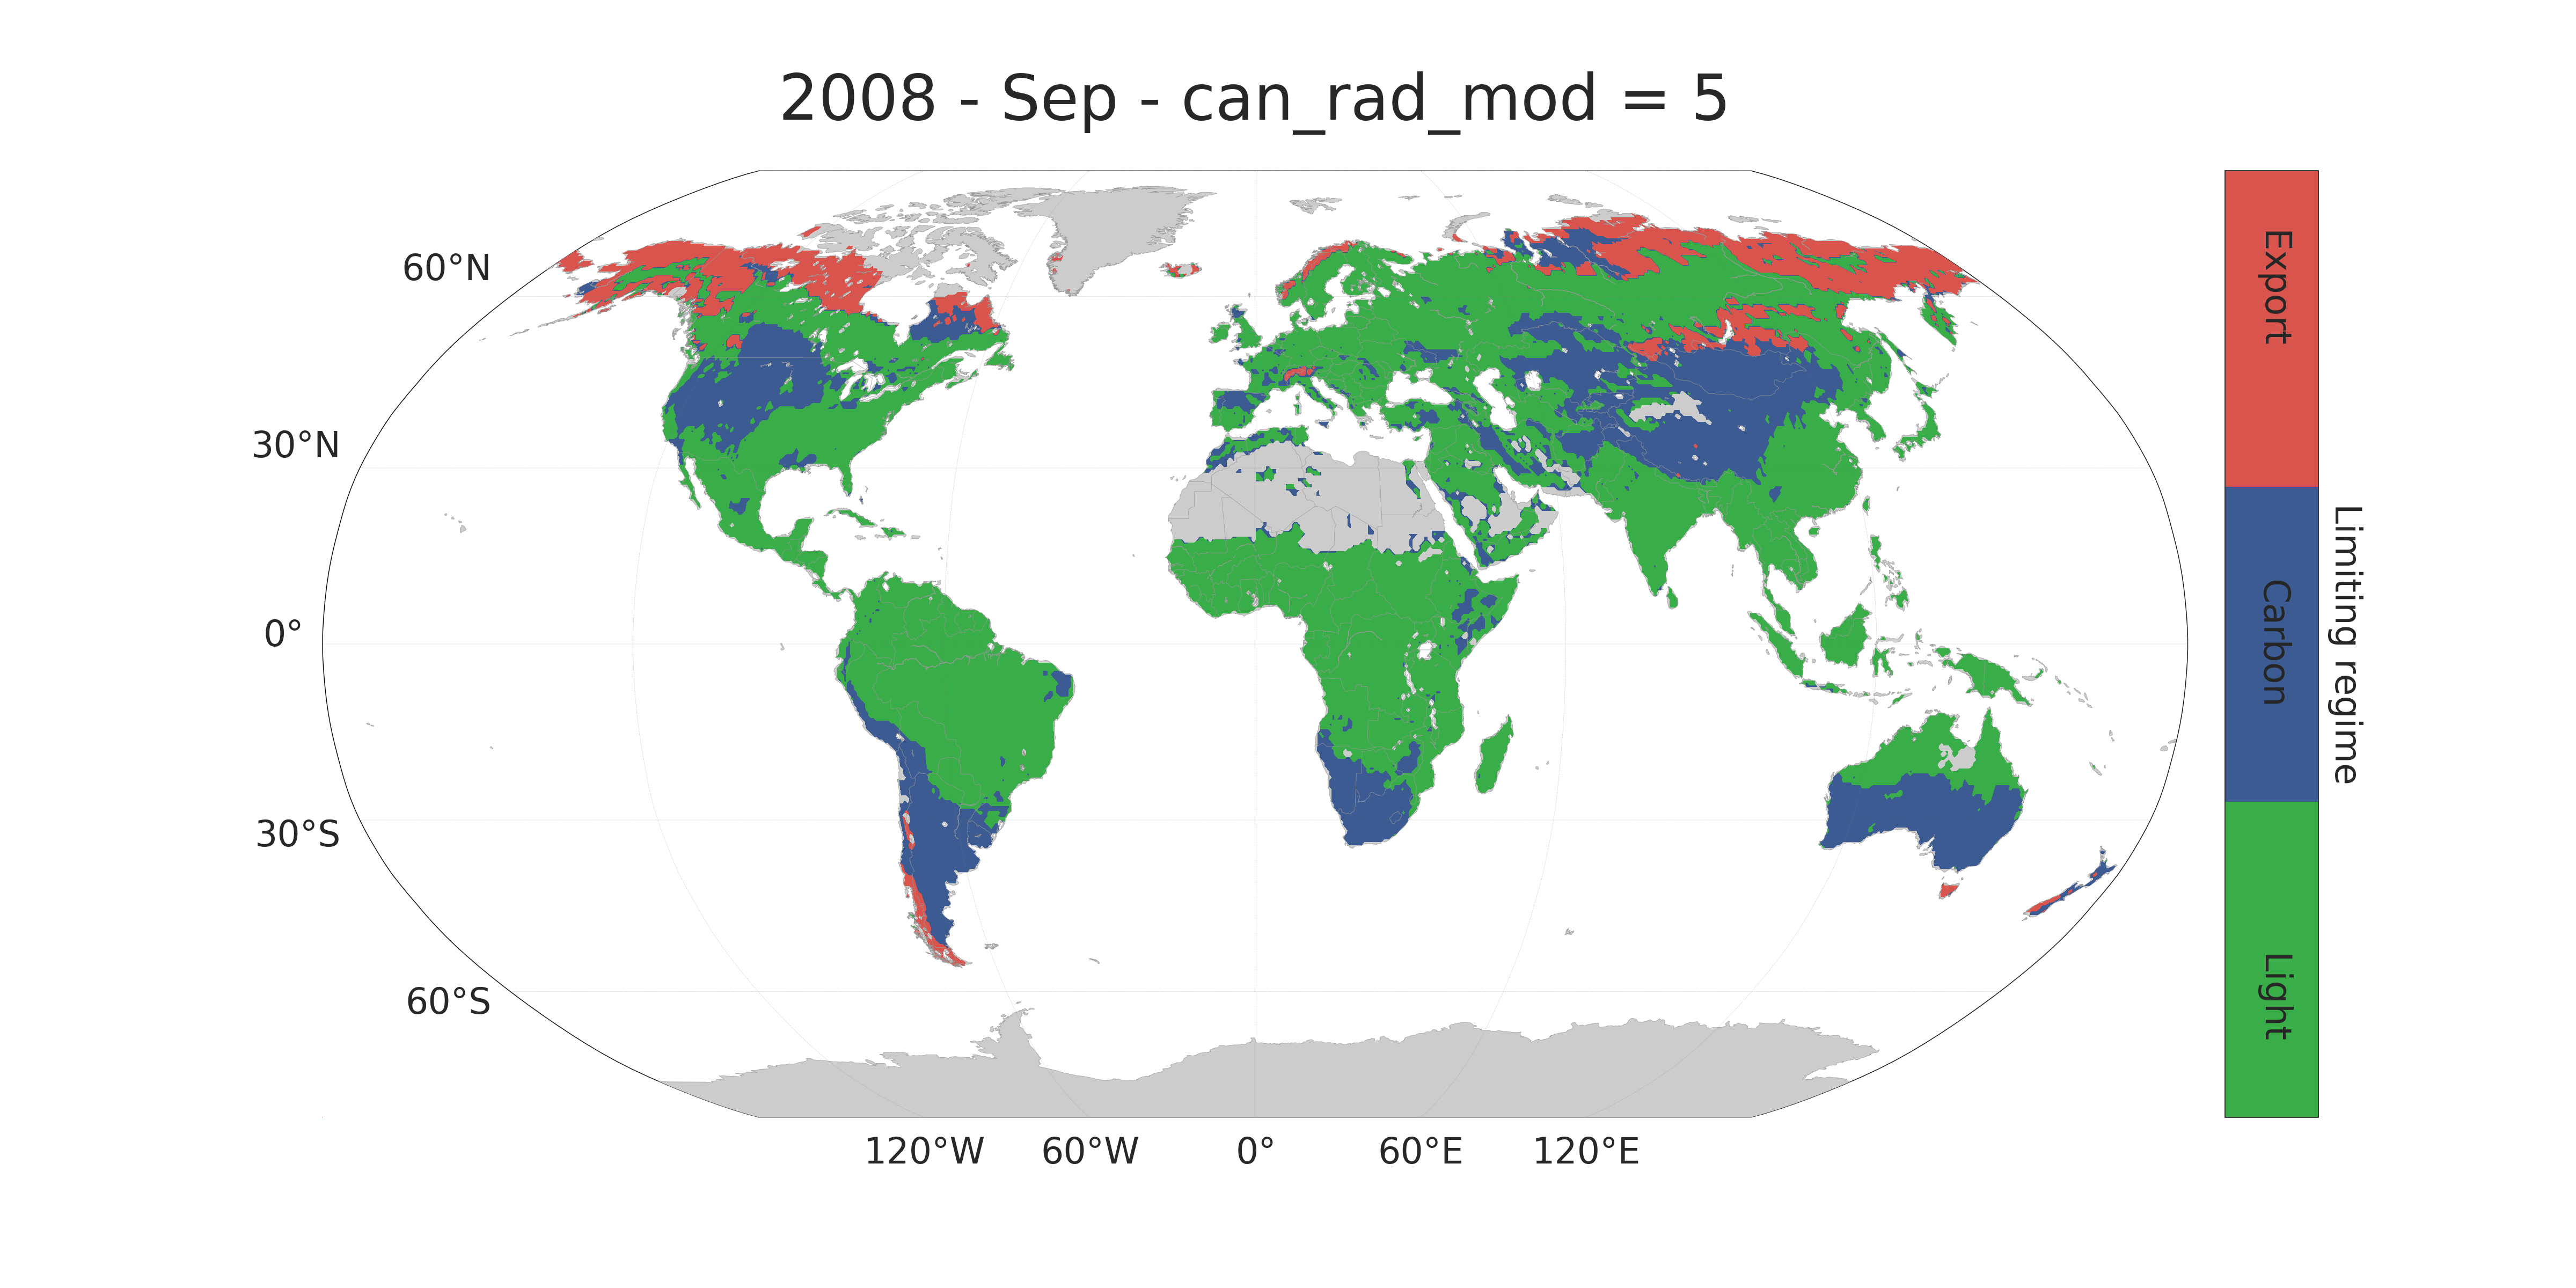
\includegraphics[width=0.33\textwidth]{/home/mn811042/Thesis/chapter6/figures_ofi/Farquhar_opt5_Sep_integral.png}}
\subfloat[Opt 5 clump]{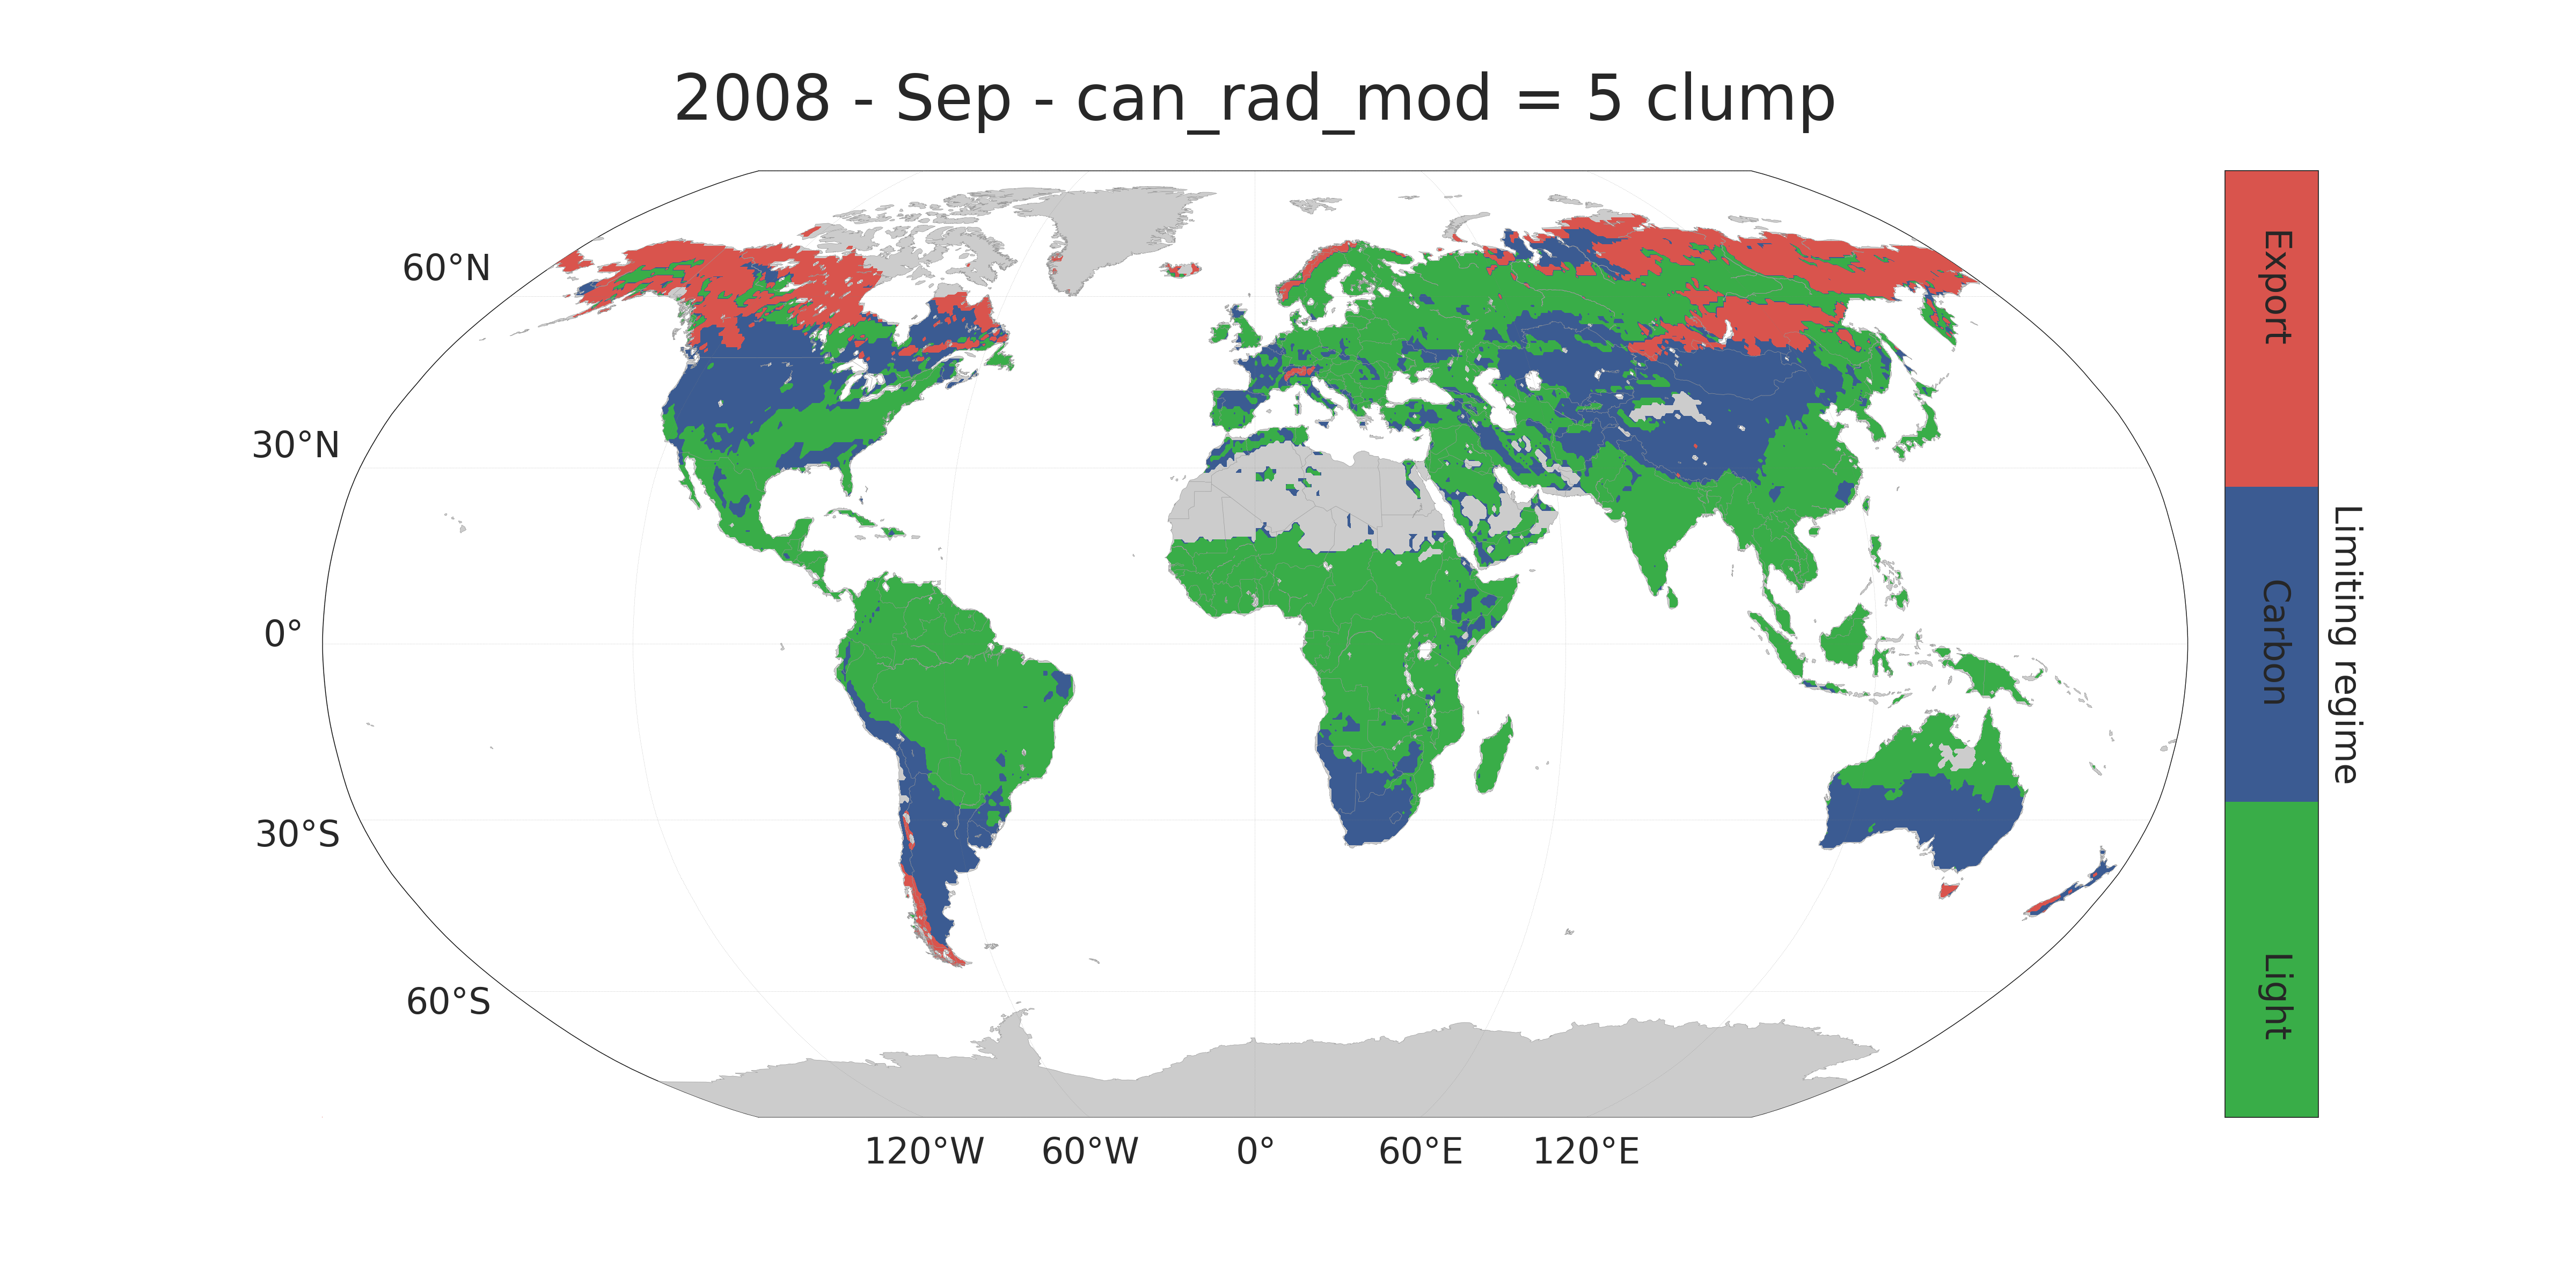
\includegraphics[width=0.33\textwidth]{/home/mn811042/Thesis/chapter6/figures_ofi/Farquhar_opt5_clump_Sep_integral.png}}
\subfloat[Difference]{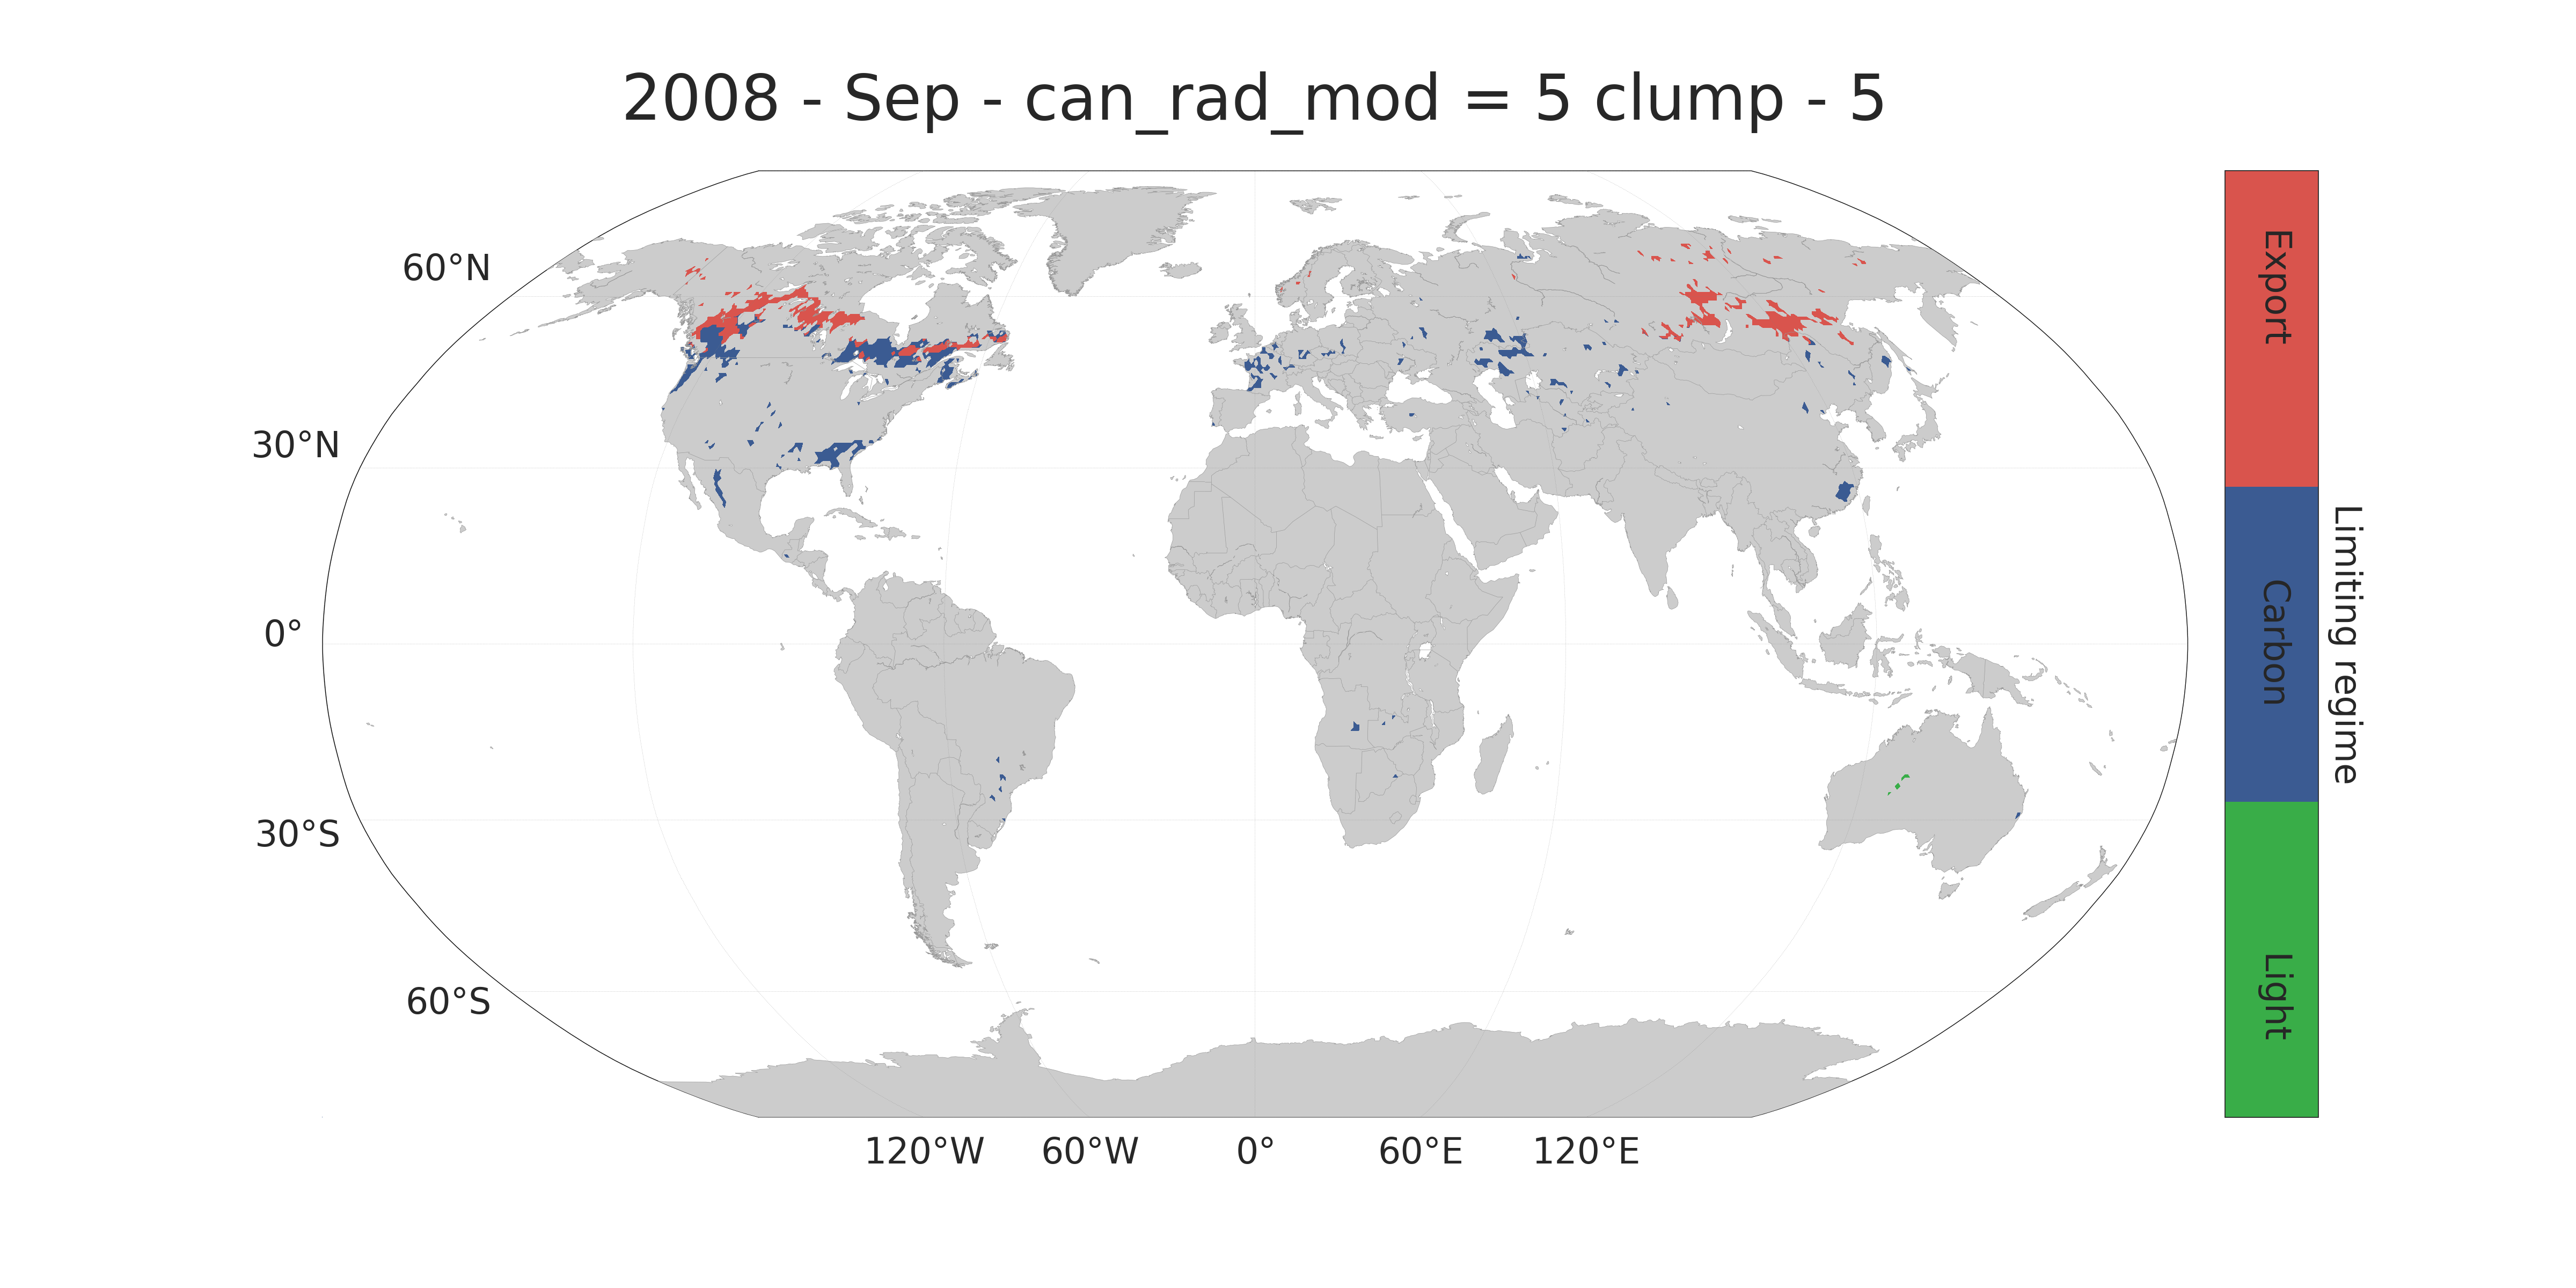
\includegraphics[width=0.33\textwidth]{/home/mn811042/Thesis/chapter6/figures_ofi/Farquhar_opt5_anomaly_Sep_integral.png}}
\end{tabular}
\begin{tabular}{lll}
\subfloat[Opt 5]{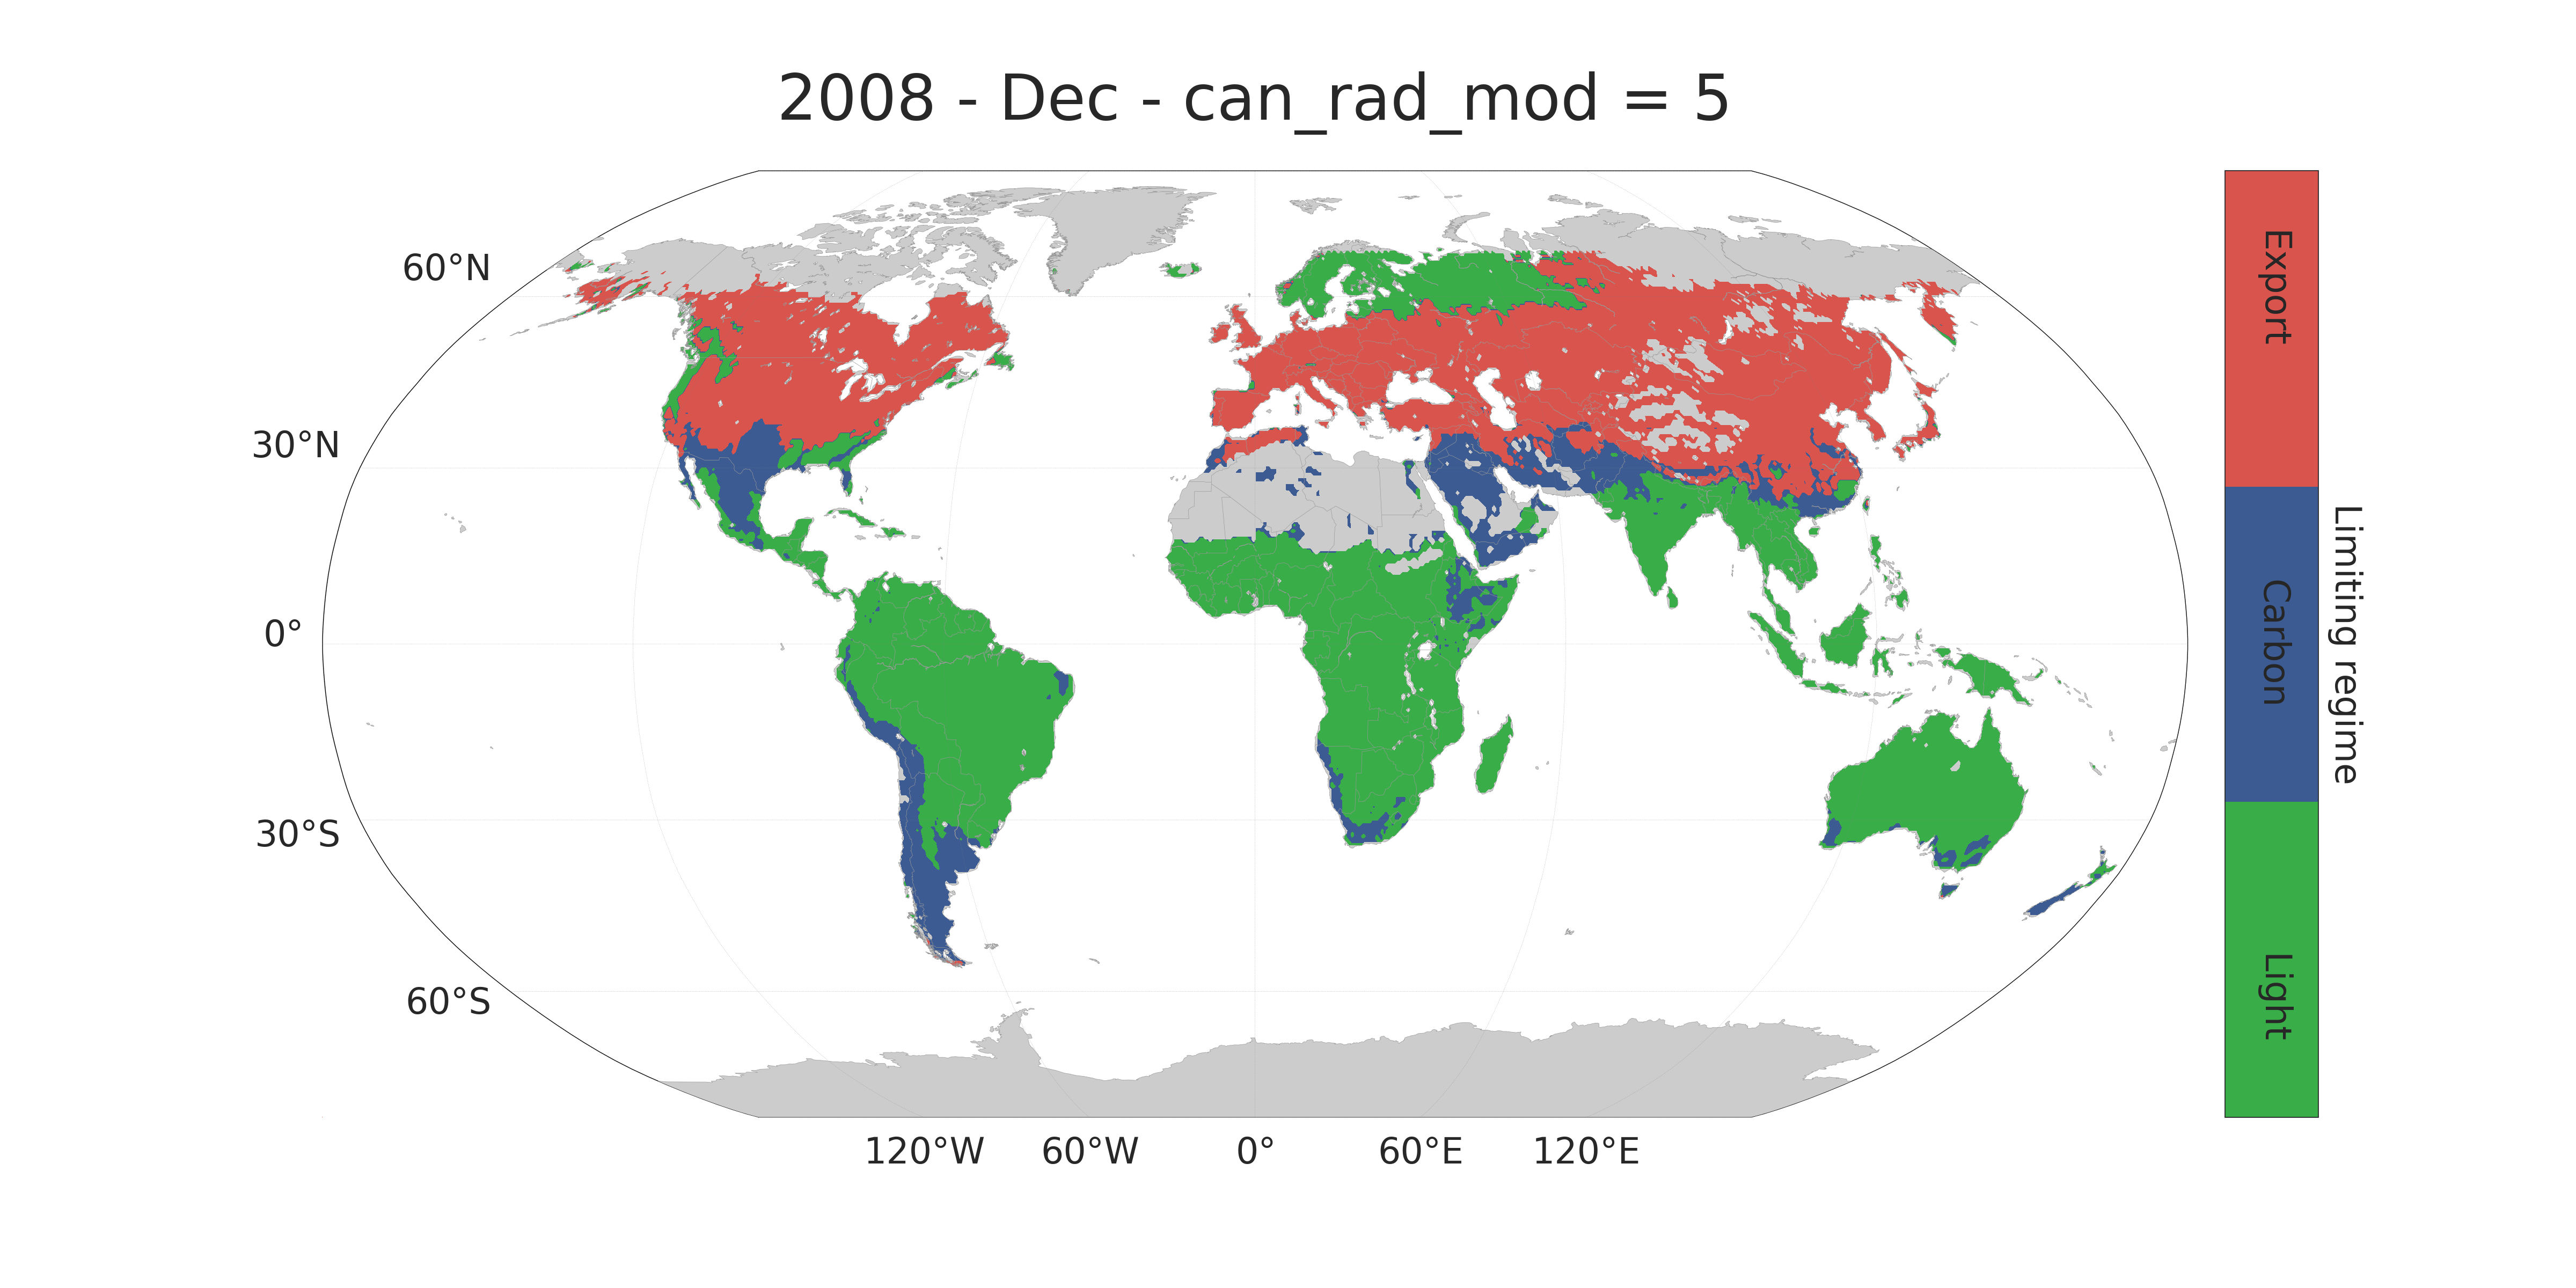
\includegraphics[width=0.33\textwidth]{/home/mn811042/Thesis/chapter6/figures_ofi/Farquhar_opt5_Dec_integral.png}}
\subfloat[Opt 5 clump]{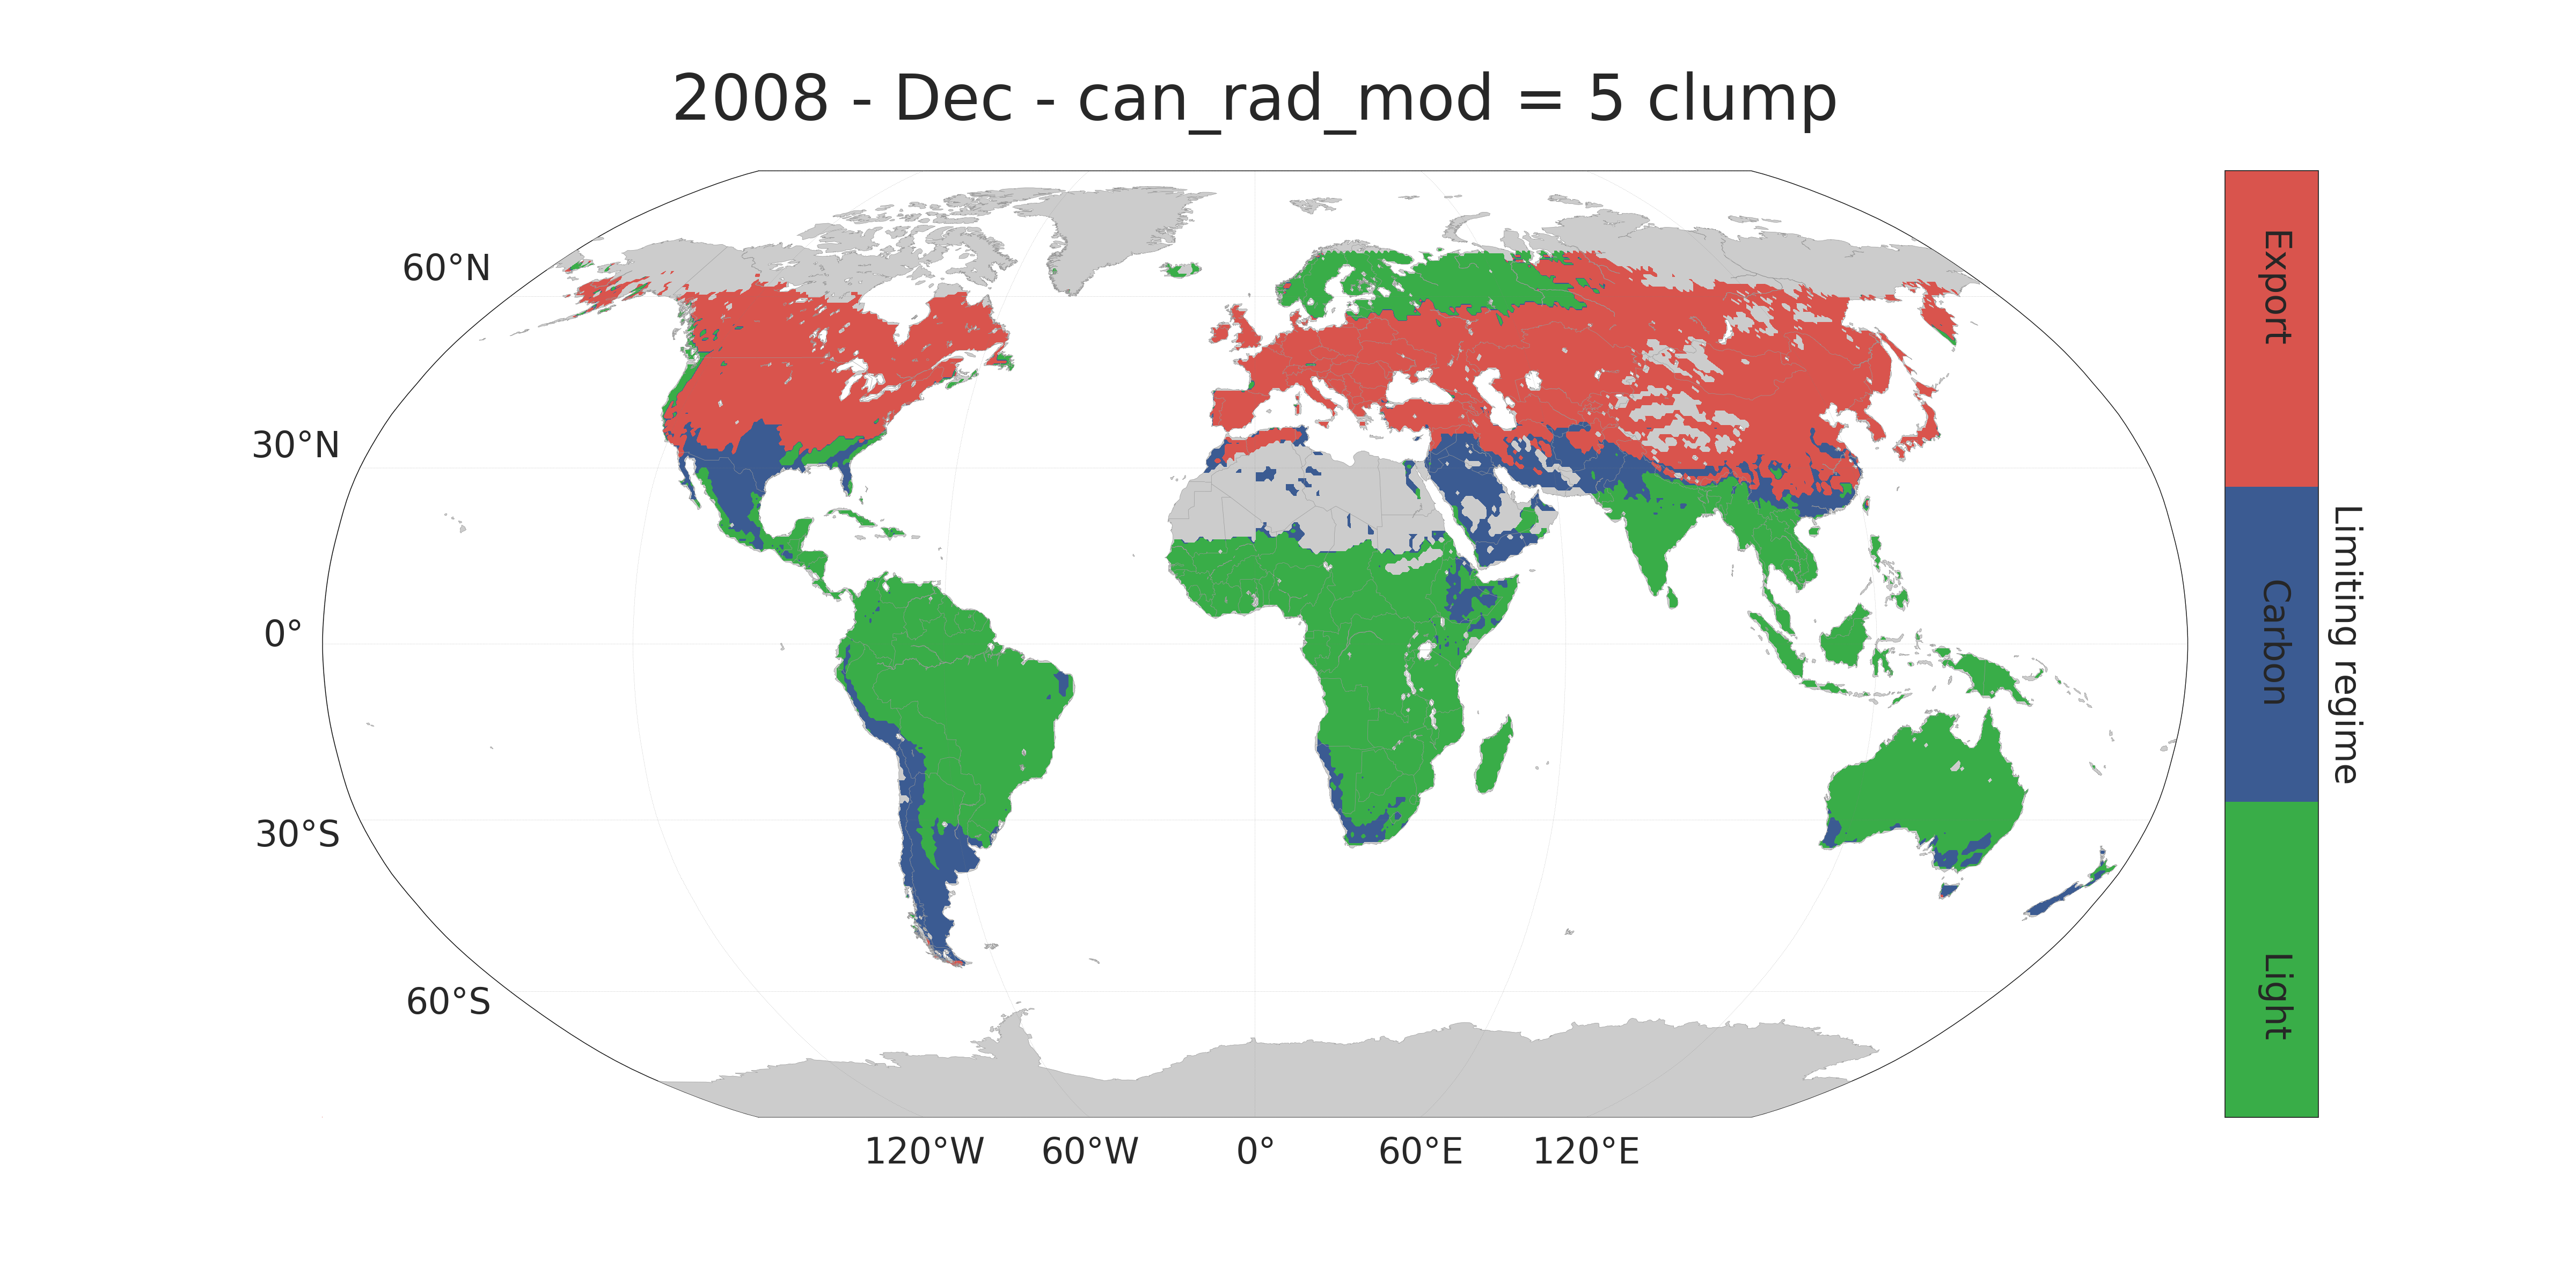
\includegraphics[width=0.33\textwidth]{/home/mn811042/Thesis/chapter6/figures_ofi/Farquhar_opt5_clump_Dec_integral.png}}
\subfloat[Difference]{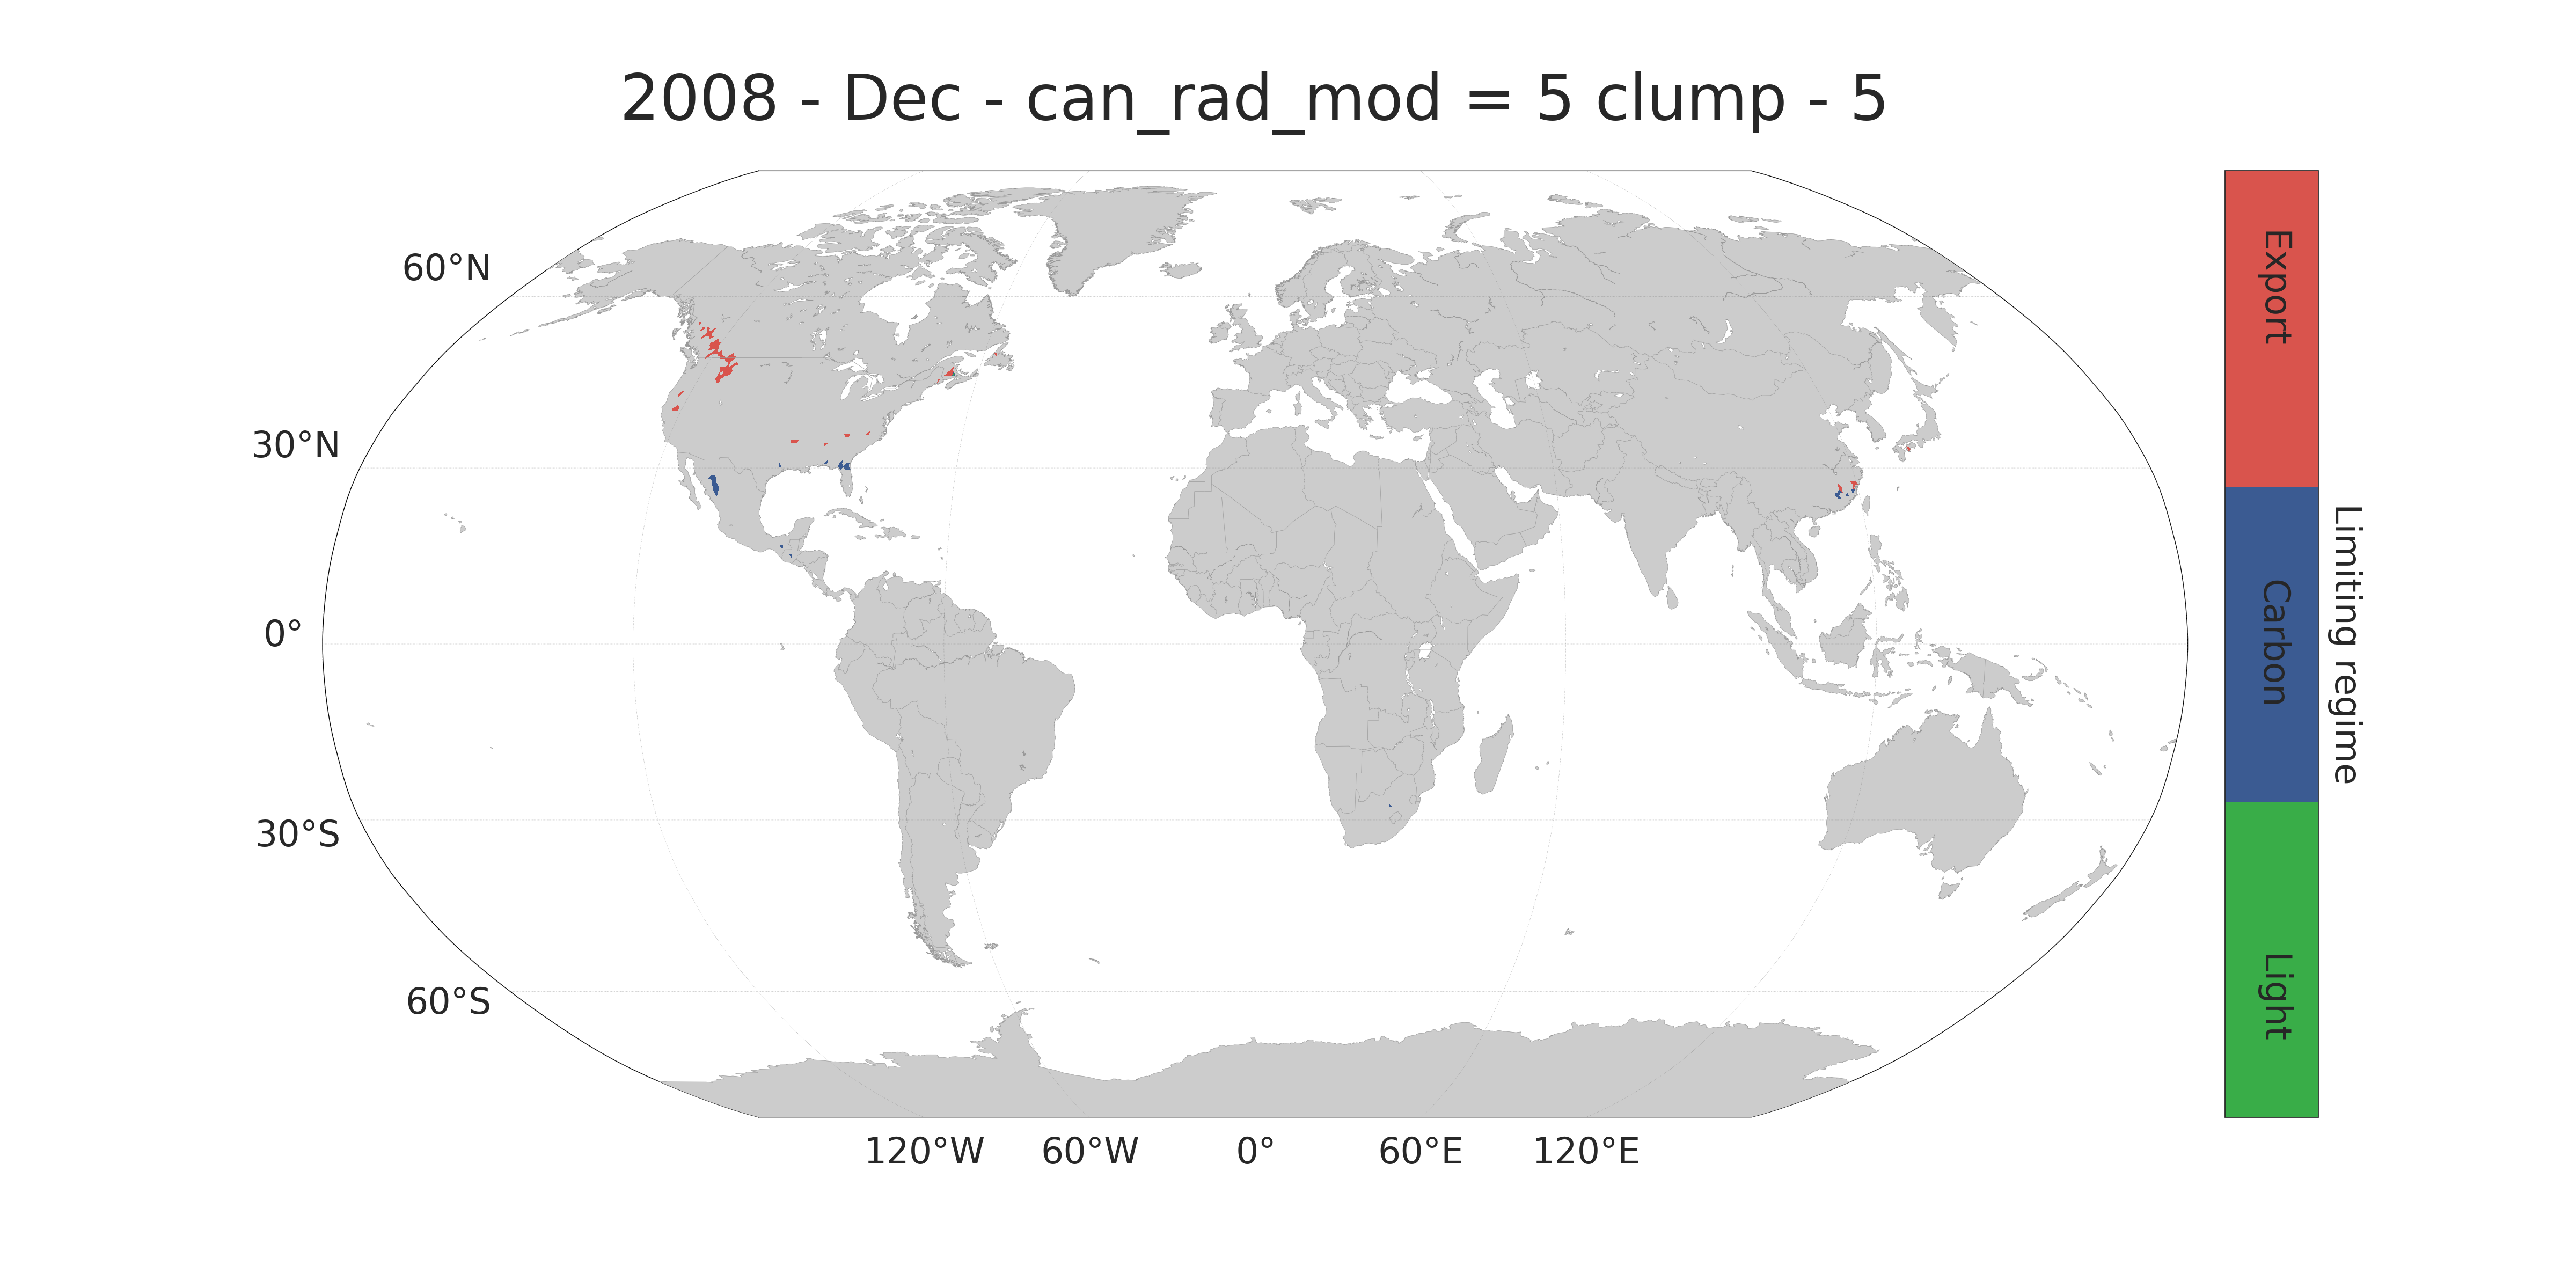
\includegraphics[width=0.33\textwidth]{/home/mn811042/Thesis/chapter6/figures_ofi/Farquhar_opt5_anomaly_Dec_integral.png}}
\end{tabular}
\caption{Average of Farquhar limiting regimes for the year of 2008.} 
\label{f:pgap}
\end{figure}

\begin{figure}[ht!]
\centering
\subfloat[MTE]{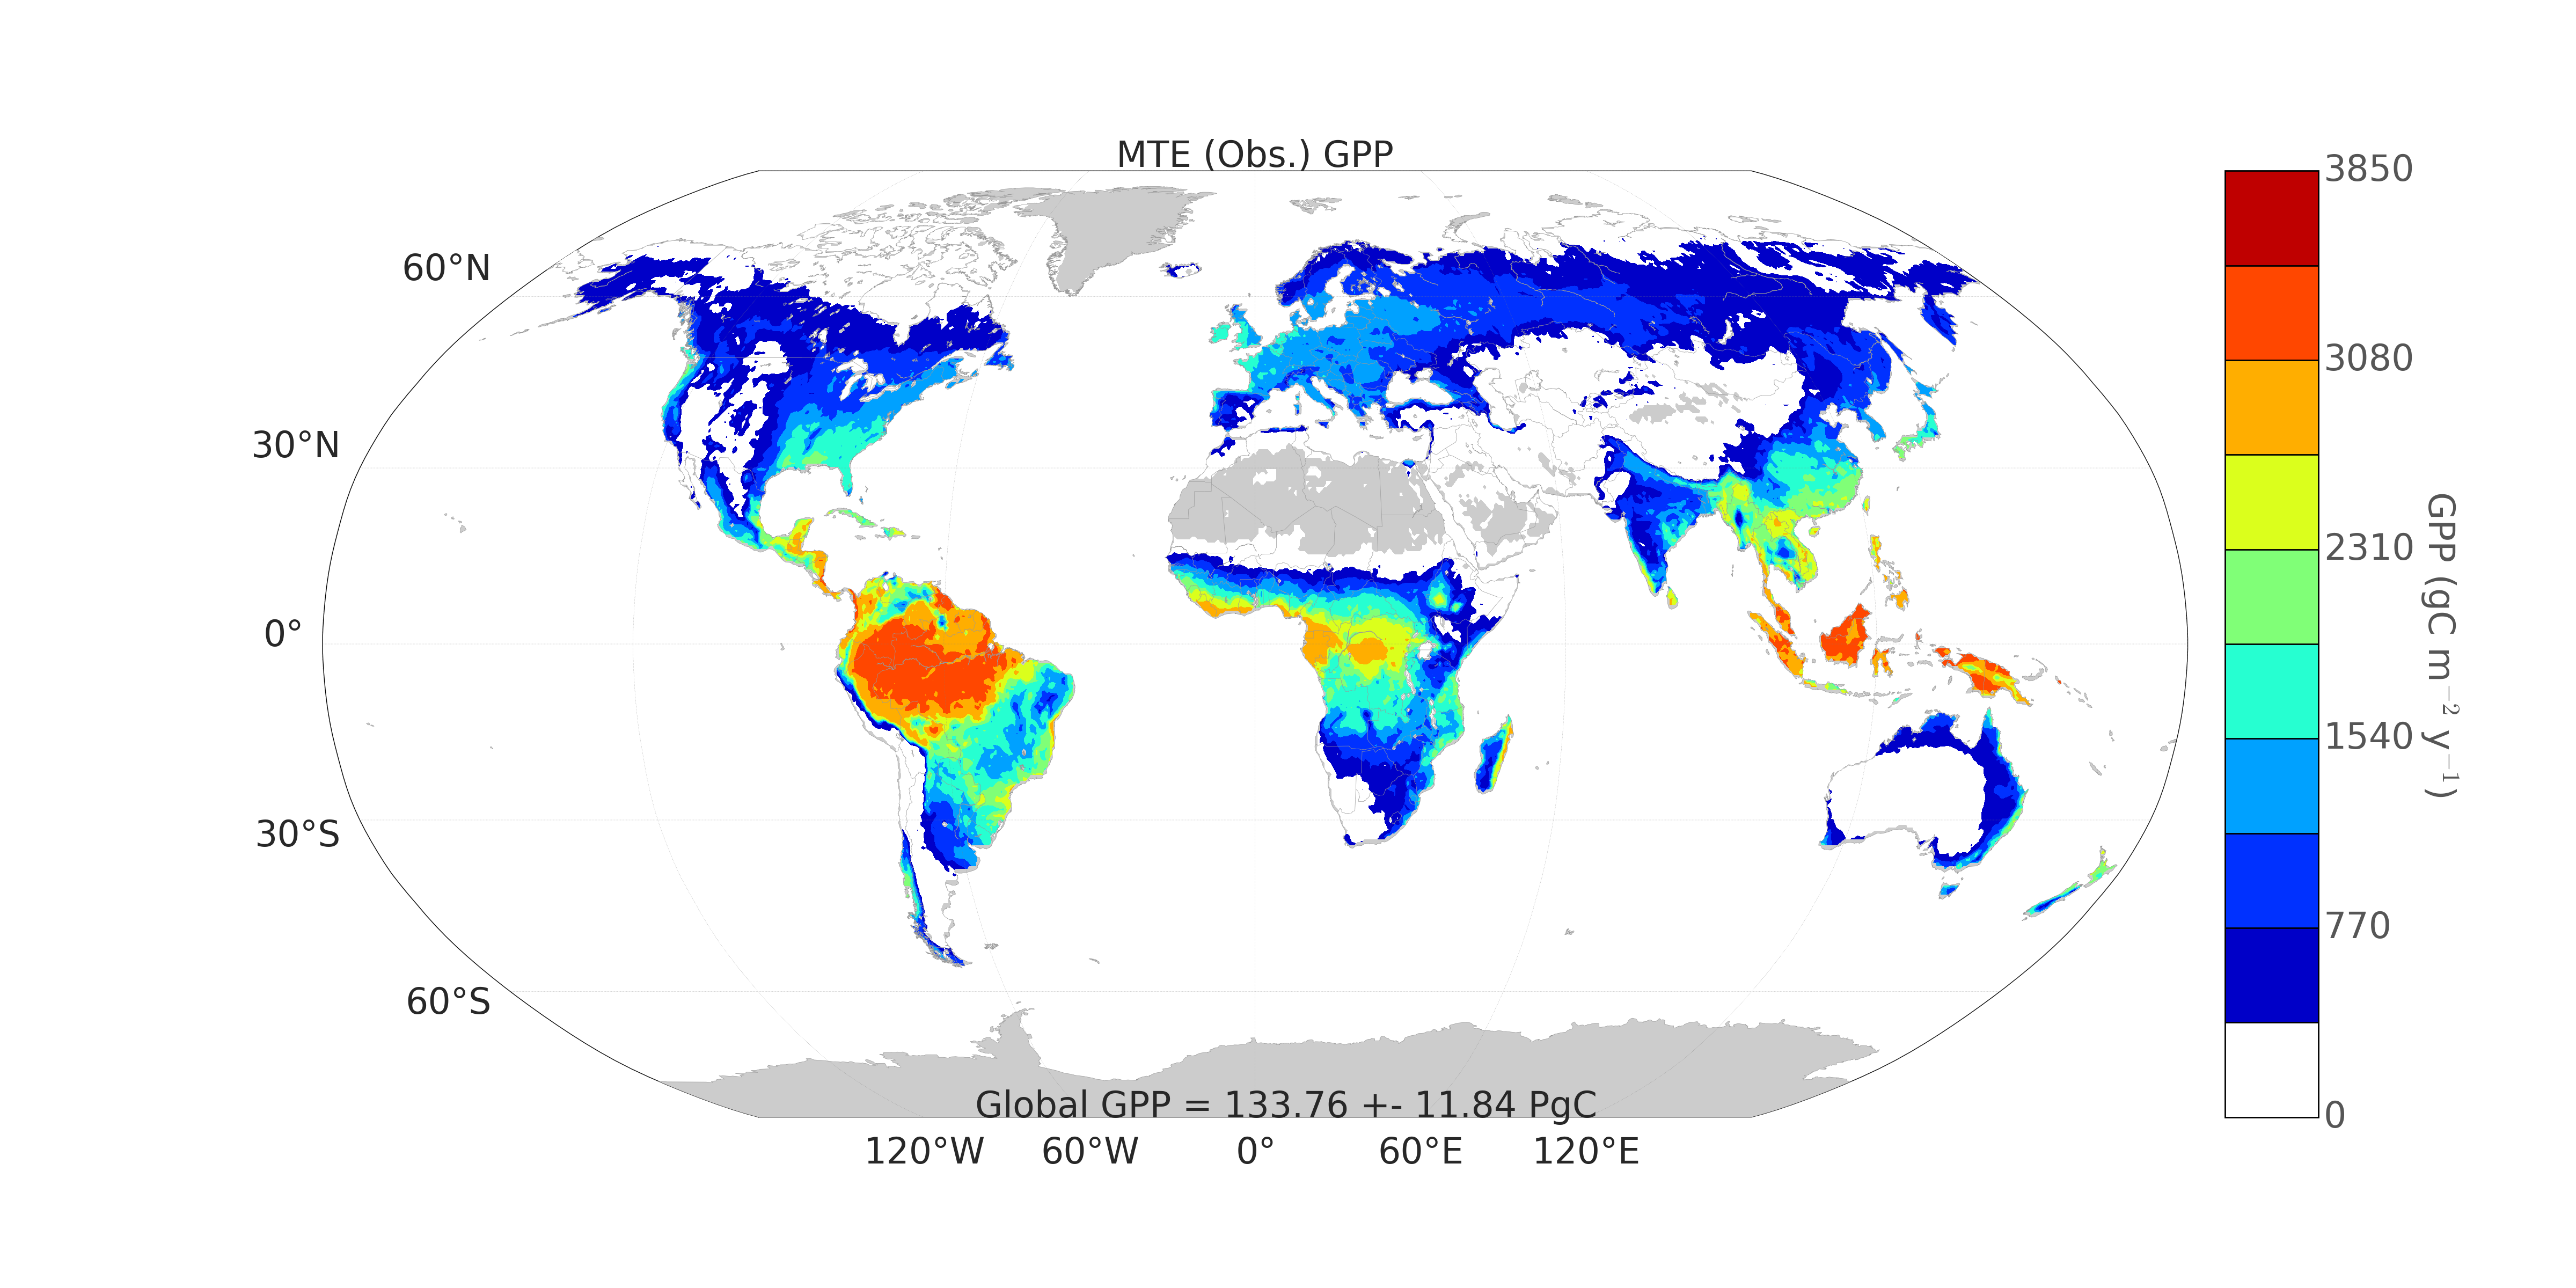
\includegraphics[width=0.8\textwidth]{/home/mn811042/Thesis/chapter6/figures_ofi/mte_0_MR_year.png}}
\begin{tabular}{ll}
\subfloat[Opt 4]{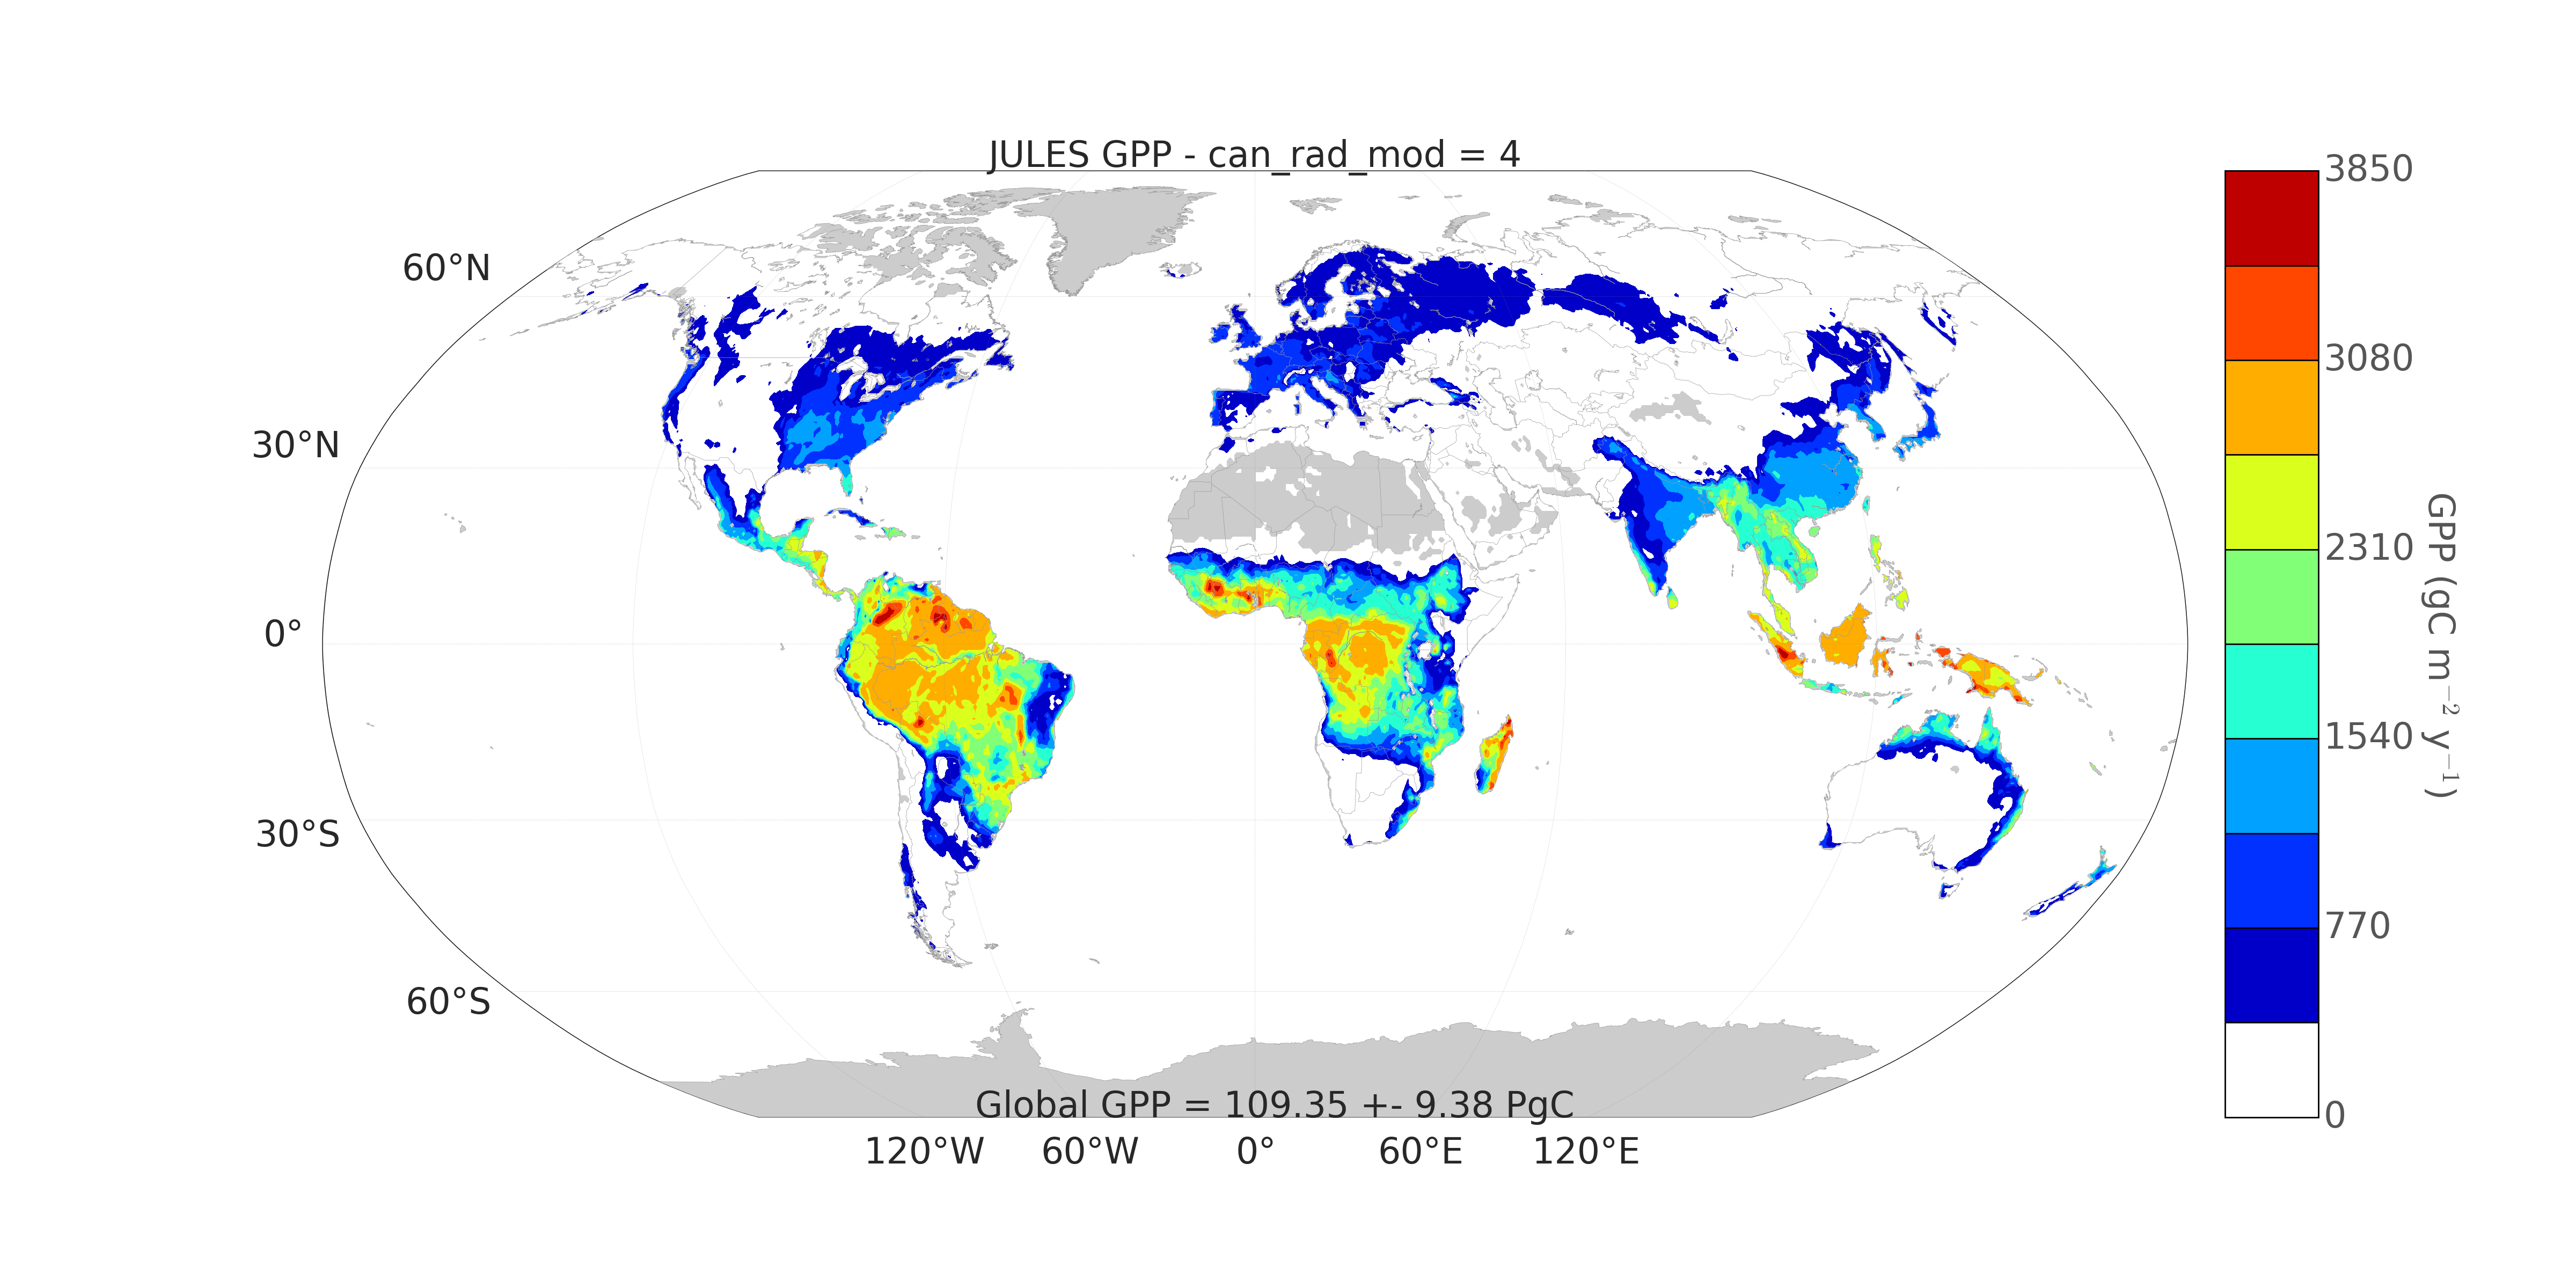
\includegraphics[width=0.5\textwidth]{/home/mn811042/Thesis/chapter6/figures_ofi/jules_opt40_MR_year.png}}
\subfloat[Opt 4 clump]{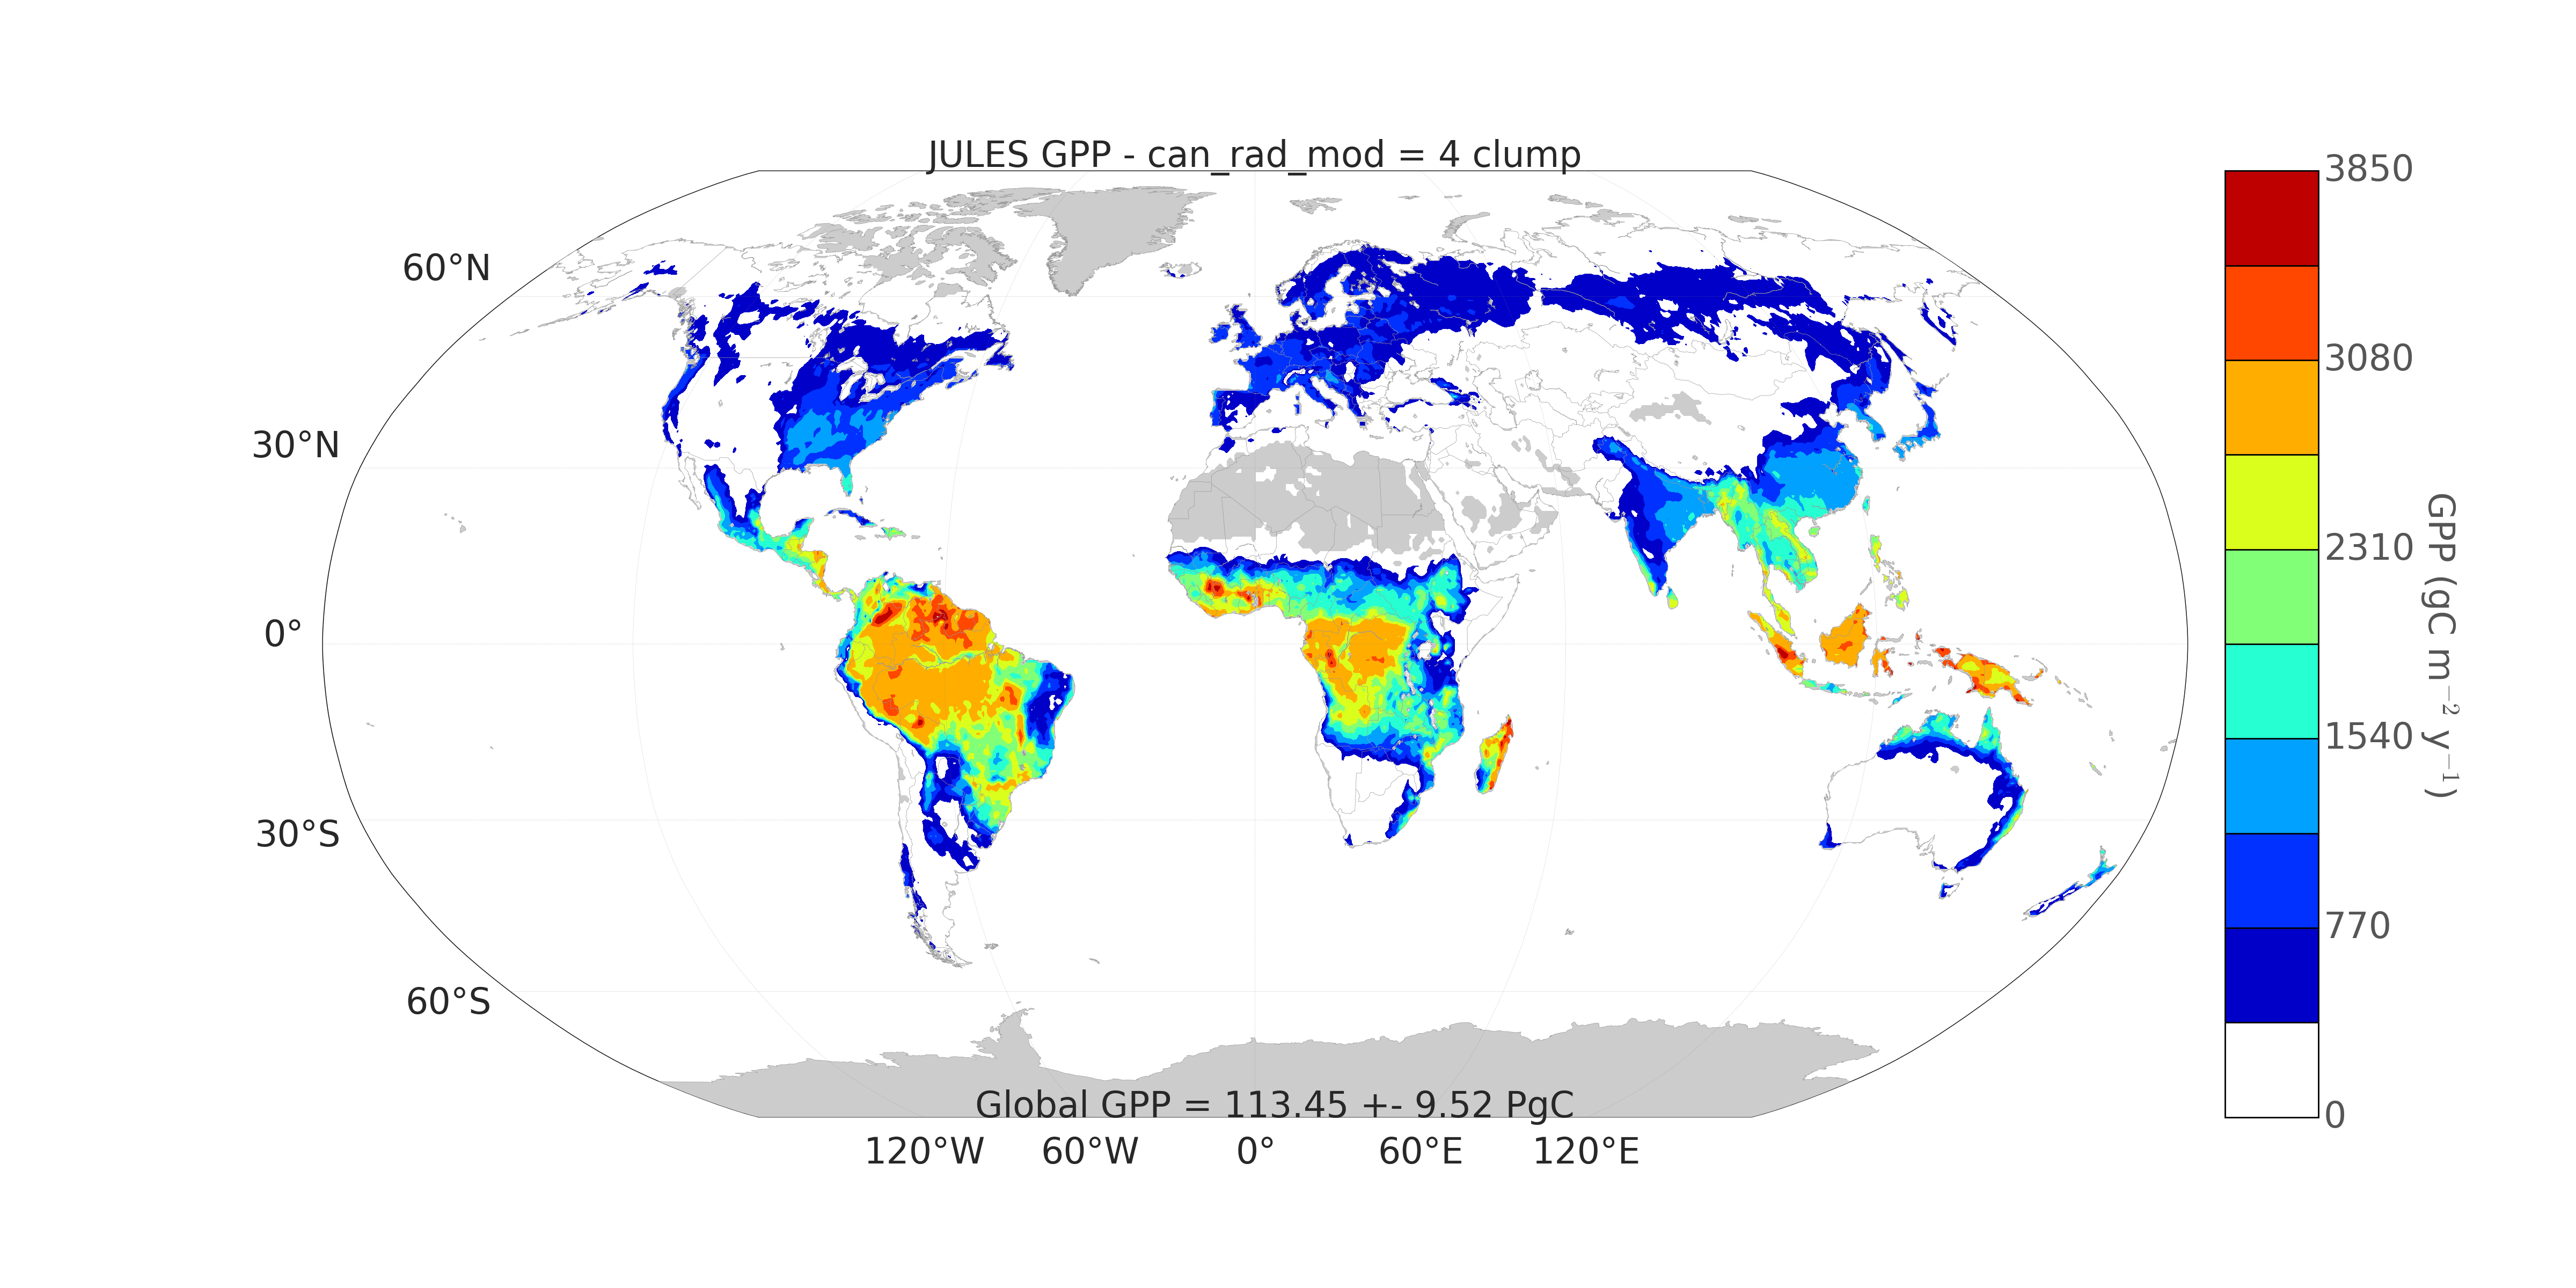
\includegraphics[width=0.5\textwidth]{/home/mn811042/Thesis/chapter6/figures_ofi/jules_opt4_clump_0_MR_year.png}}
\end{tabular}
\begin{tabular}{ll}
\subfloat[Opt 5]{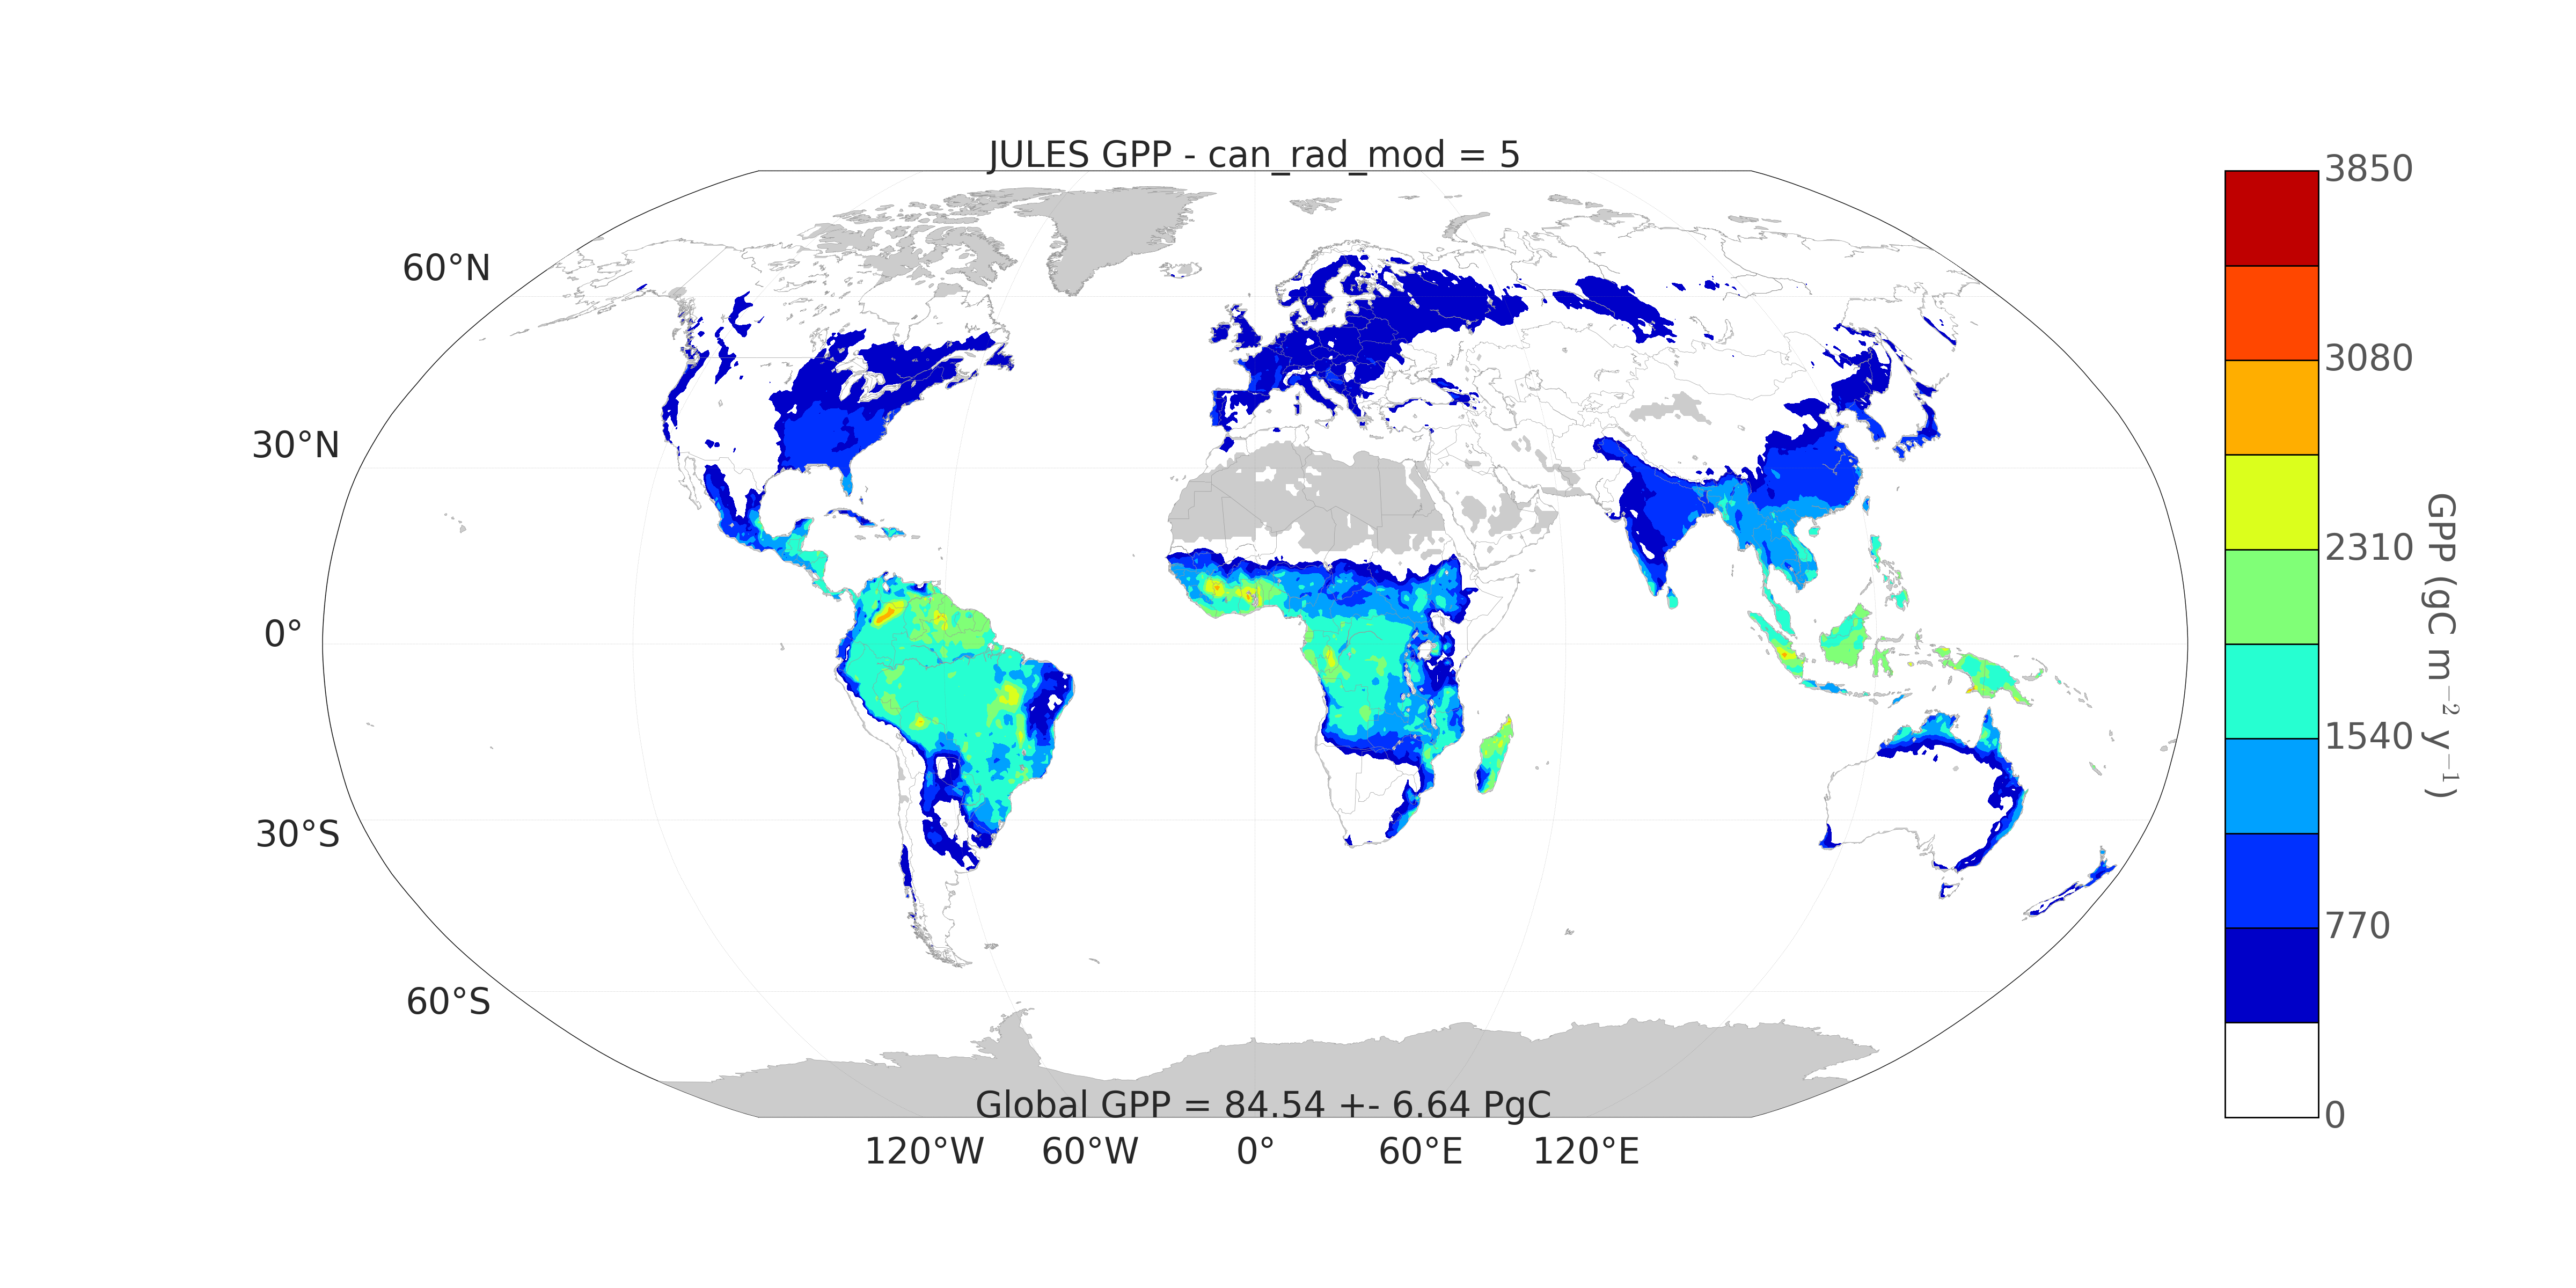
\includegraphics[width=0.5\textwidth]{/home/mn811042/Thesis/chapter6/figures_ofi/jules_opt5_0_MR_year.png}}
\subfloat[Opt 5 clump]{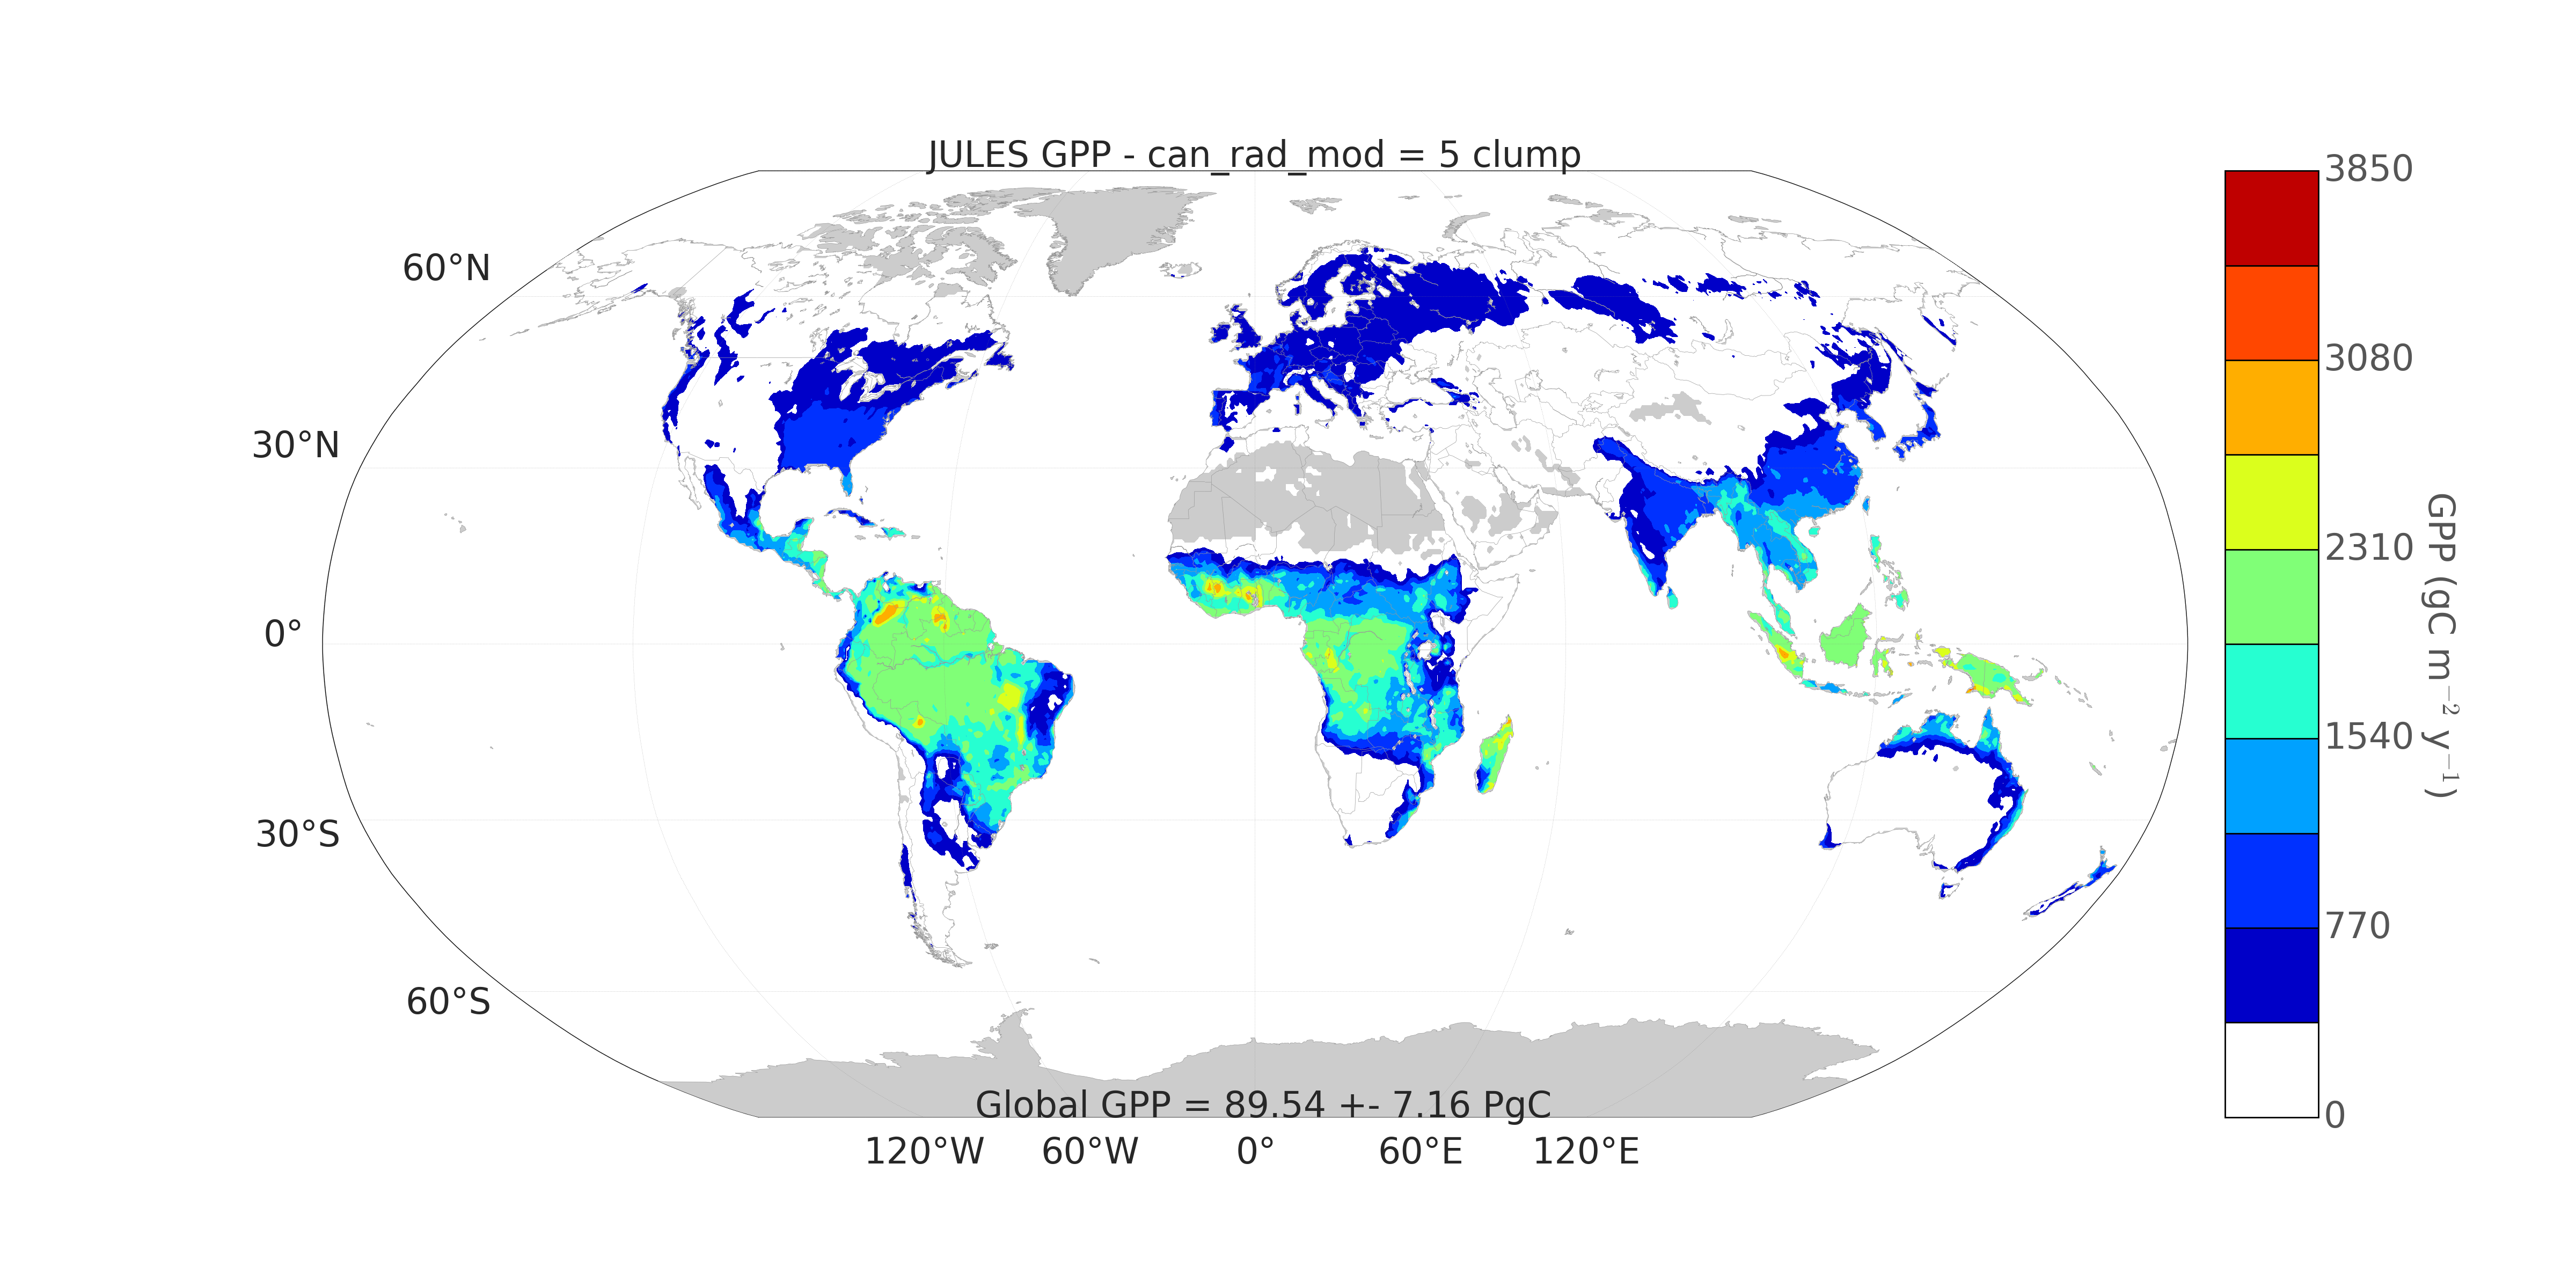
\includegraphics[width=0.5\textwidth]{/home/mn811042/Thesis/chapter6/figures_ofi/jules_opt5_clump_0_MR_year.png}}
\end{tabular}
\begin{tabular}{ll}
\subfloat[Opt 4 - MTE]{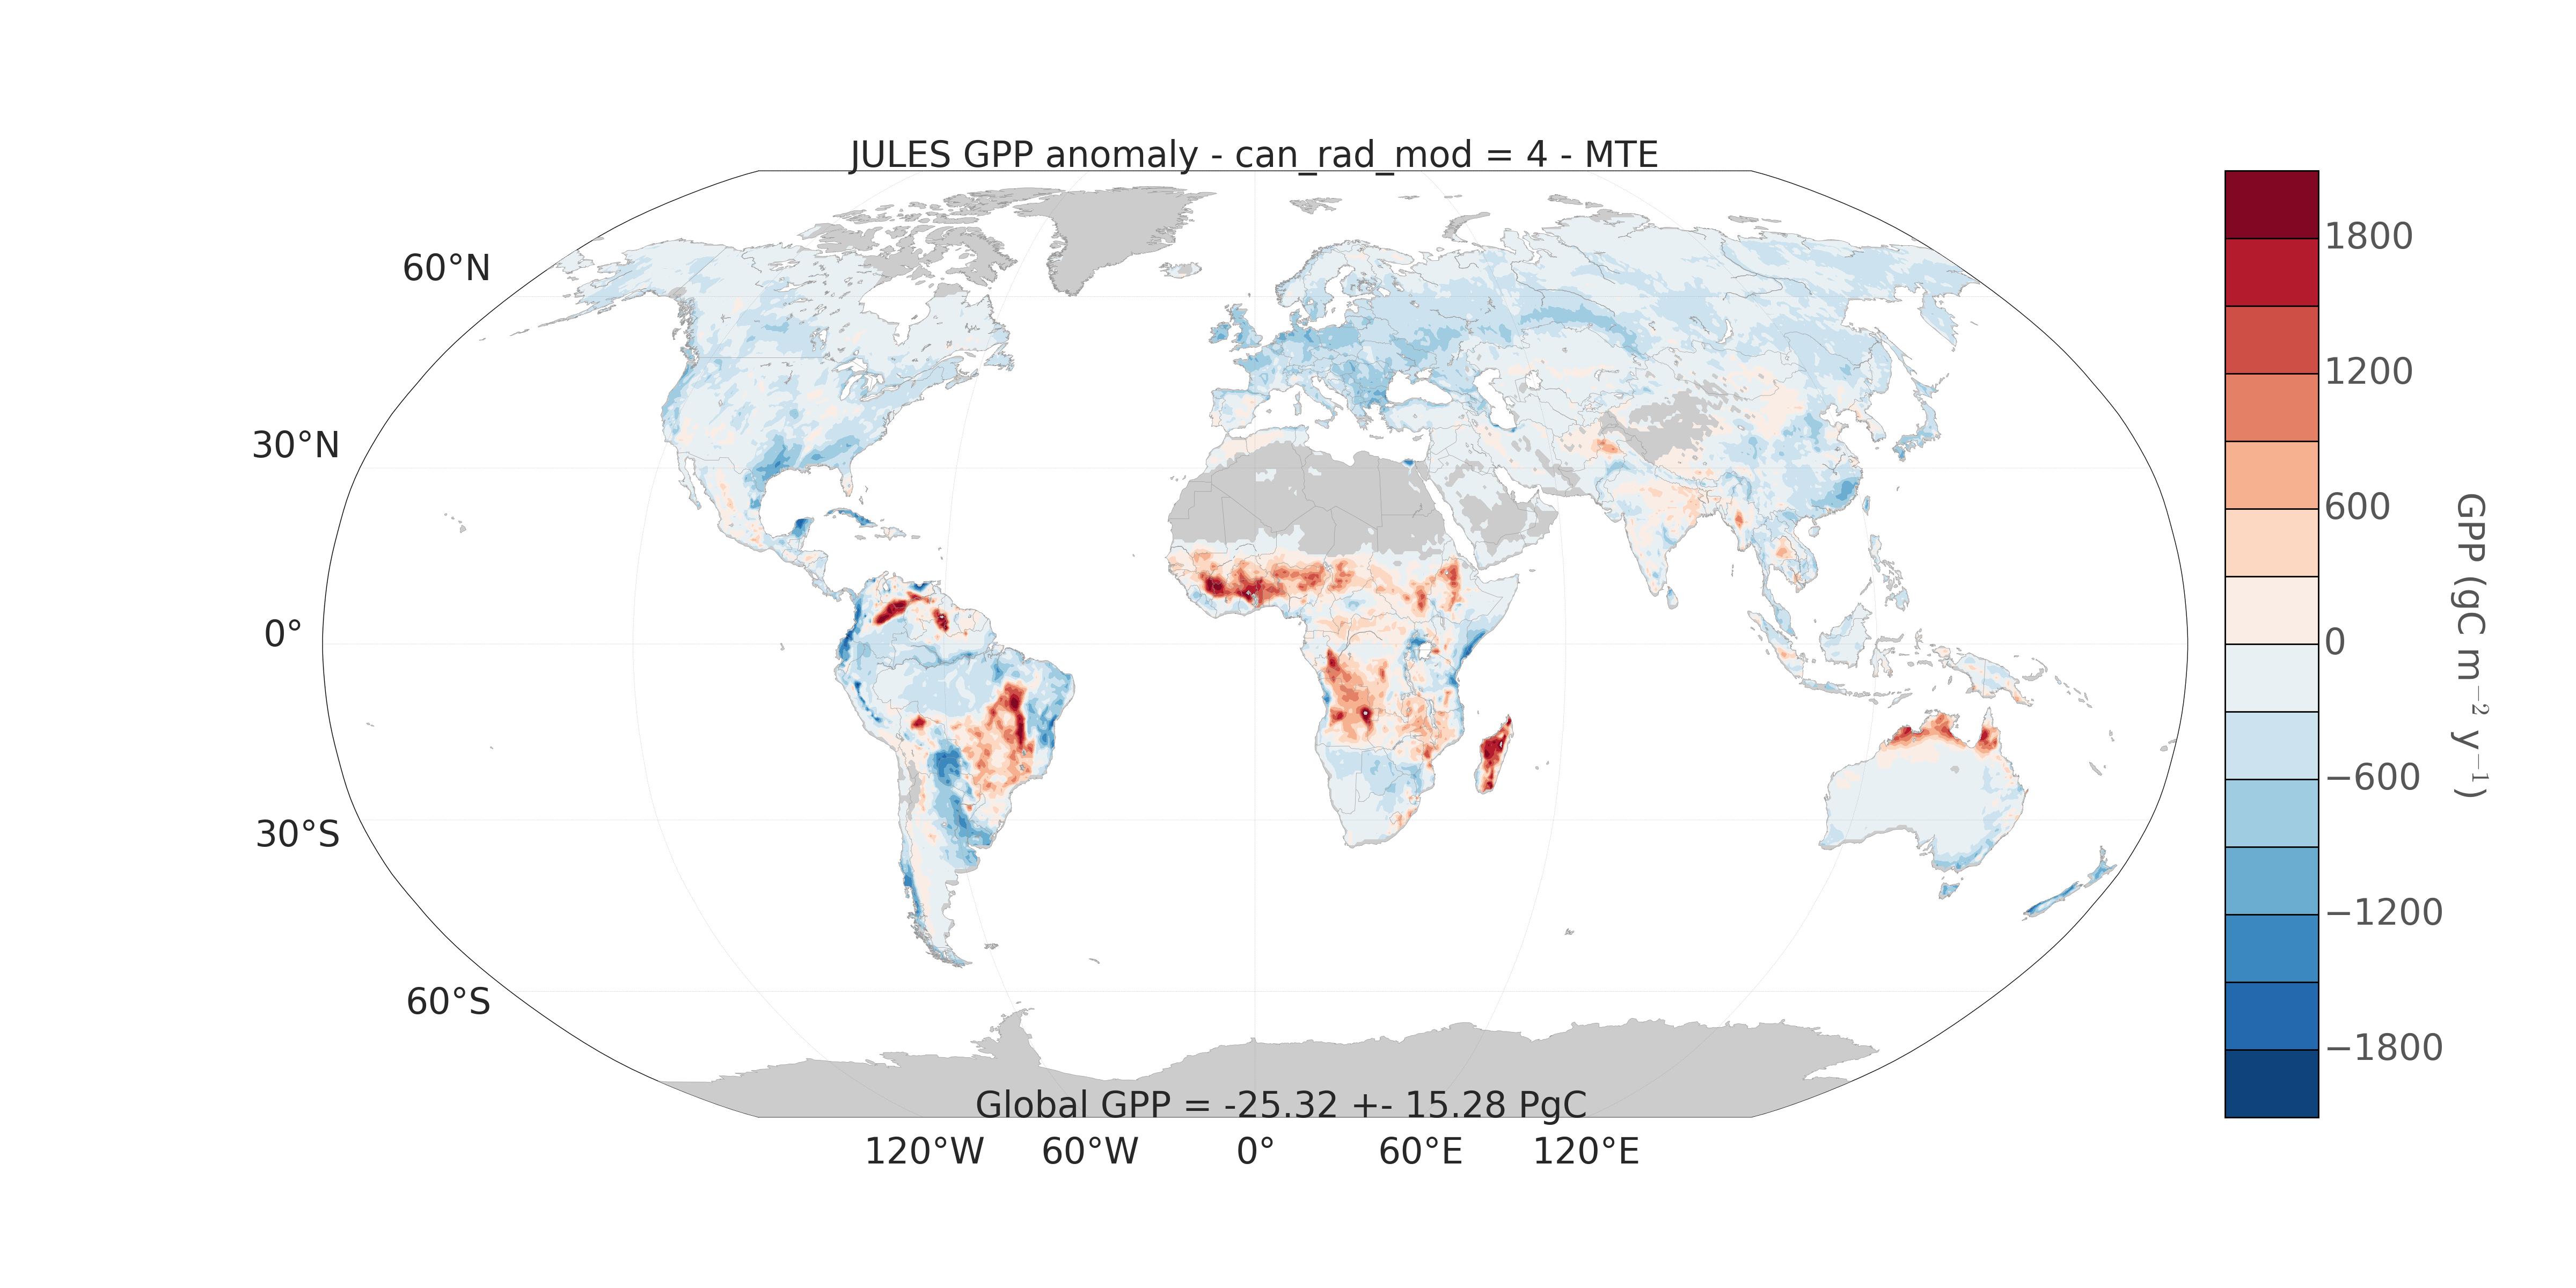
\includegraphics[width=0.5\textwidth]{/home/mn811042/Thesis/chapter6/figures_ofi/jules_mte_anom_opt40_MR_year.png}}
\subfloat[Opt 4 clump - MTE]{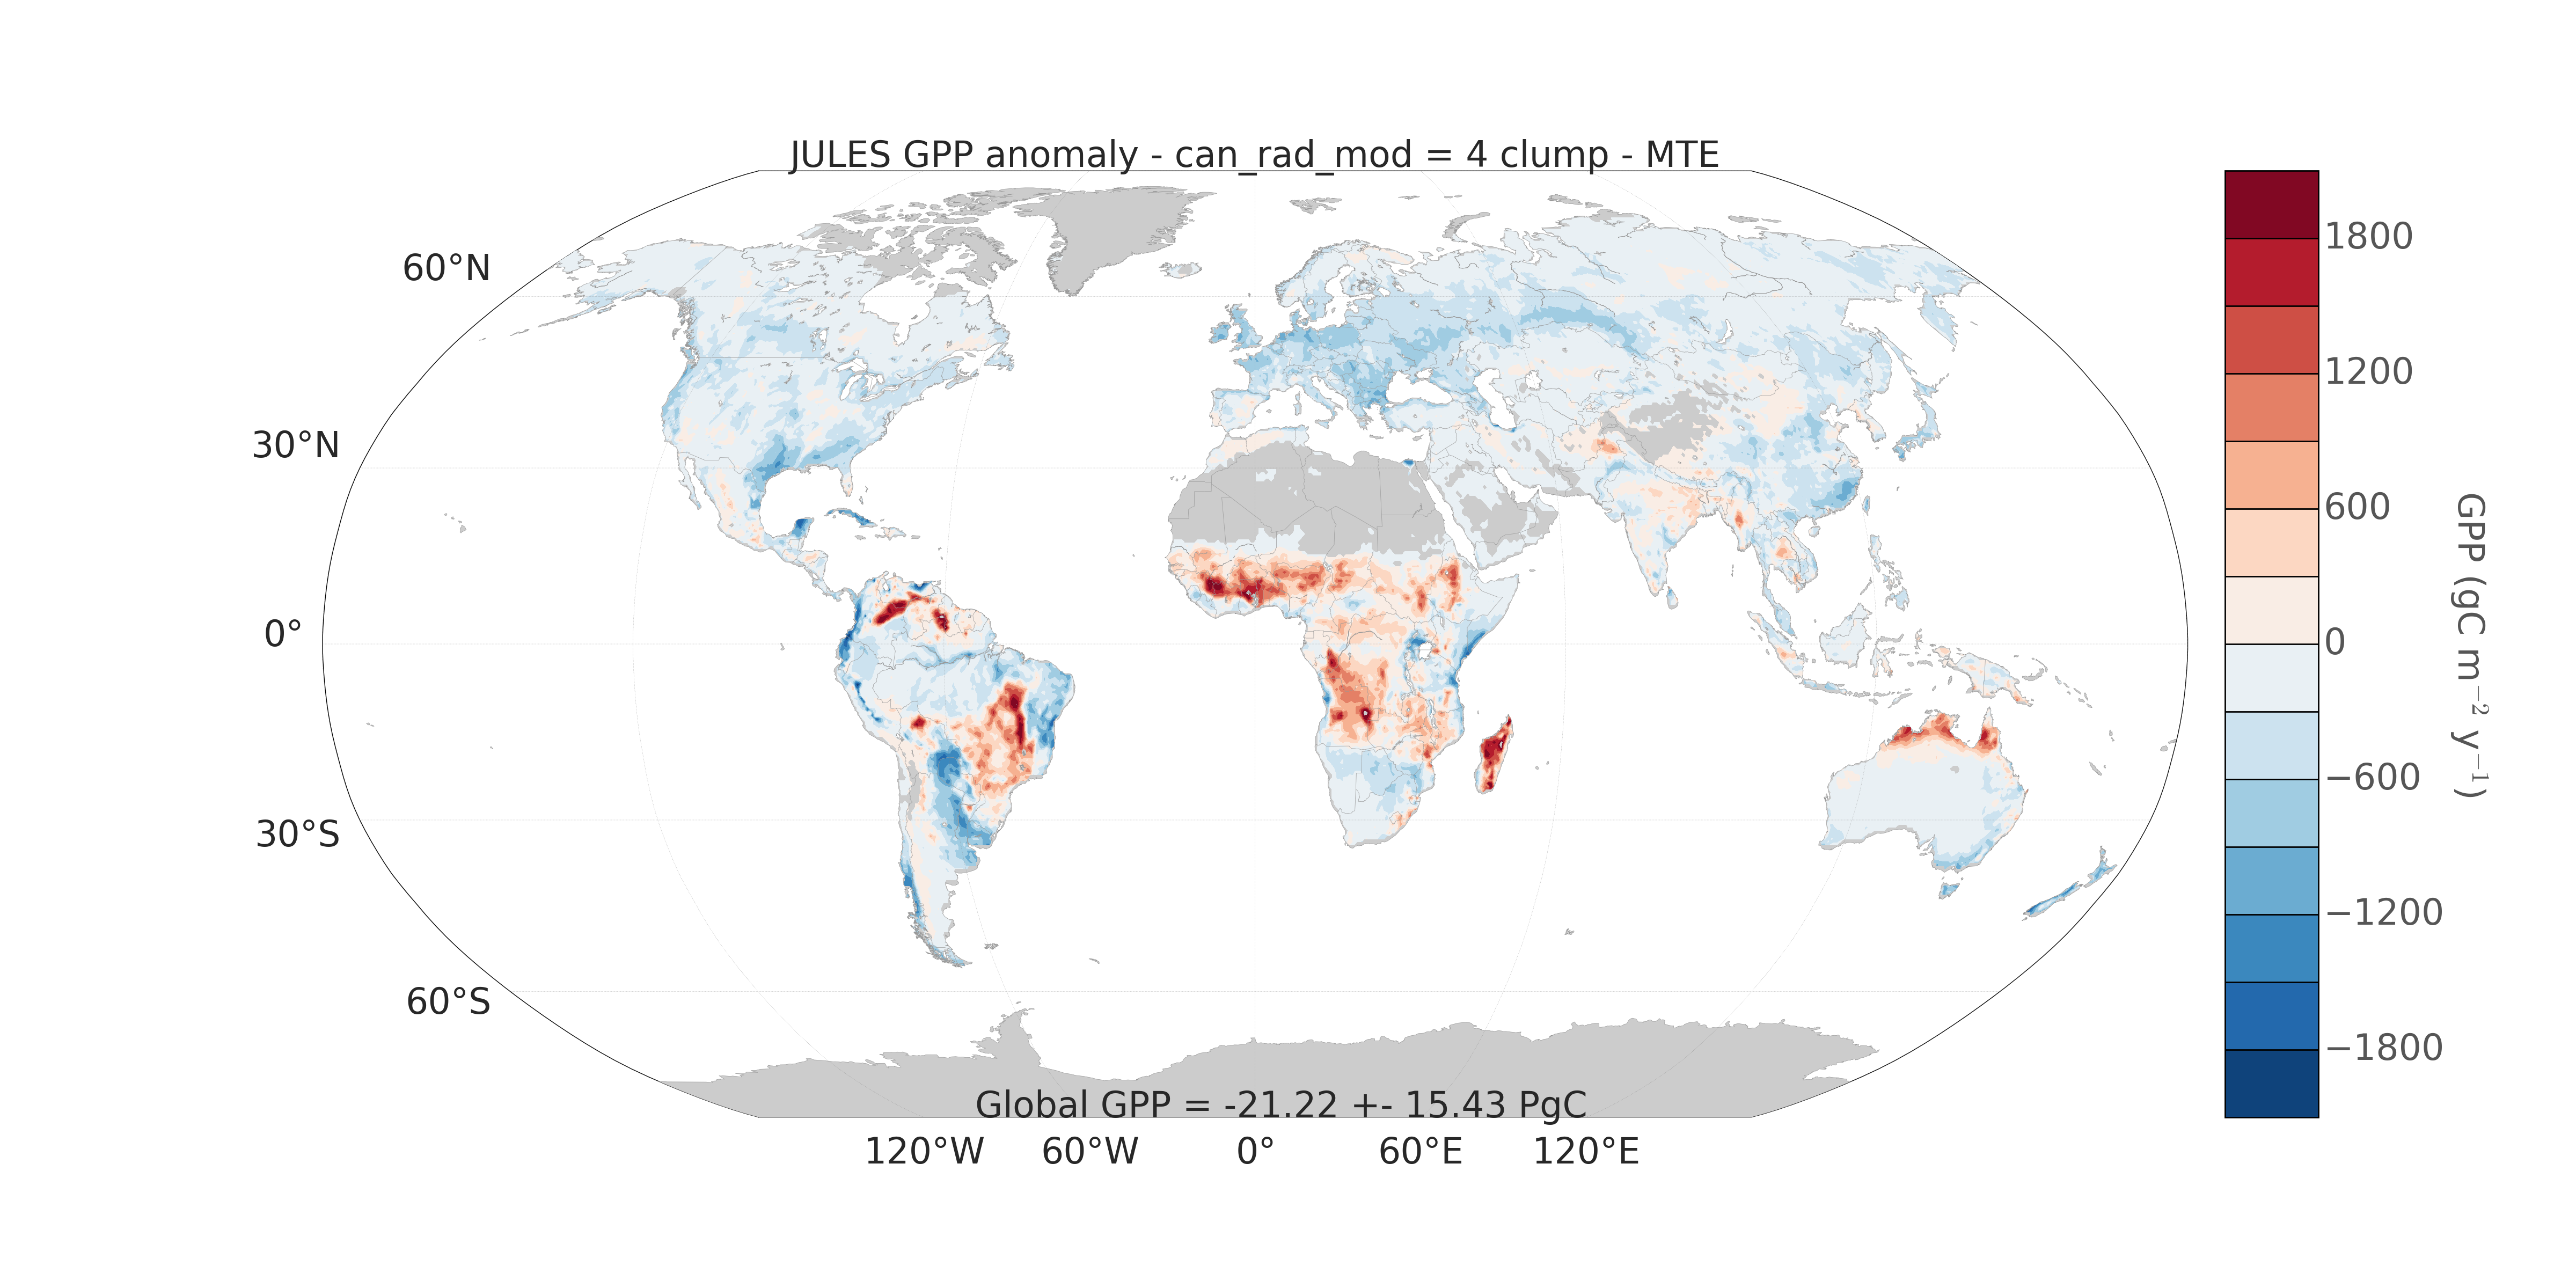
\includegraphics[width=0.5\textwidth]{/home/mn811042/Thesis/chapter6/figures_ofi/jules_mte_anom_opt40_clump_MR_year.png}}
\end{tabular}
\begin{tabular}{ll}
\subfloat[Opt 5 - MTE]{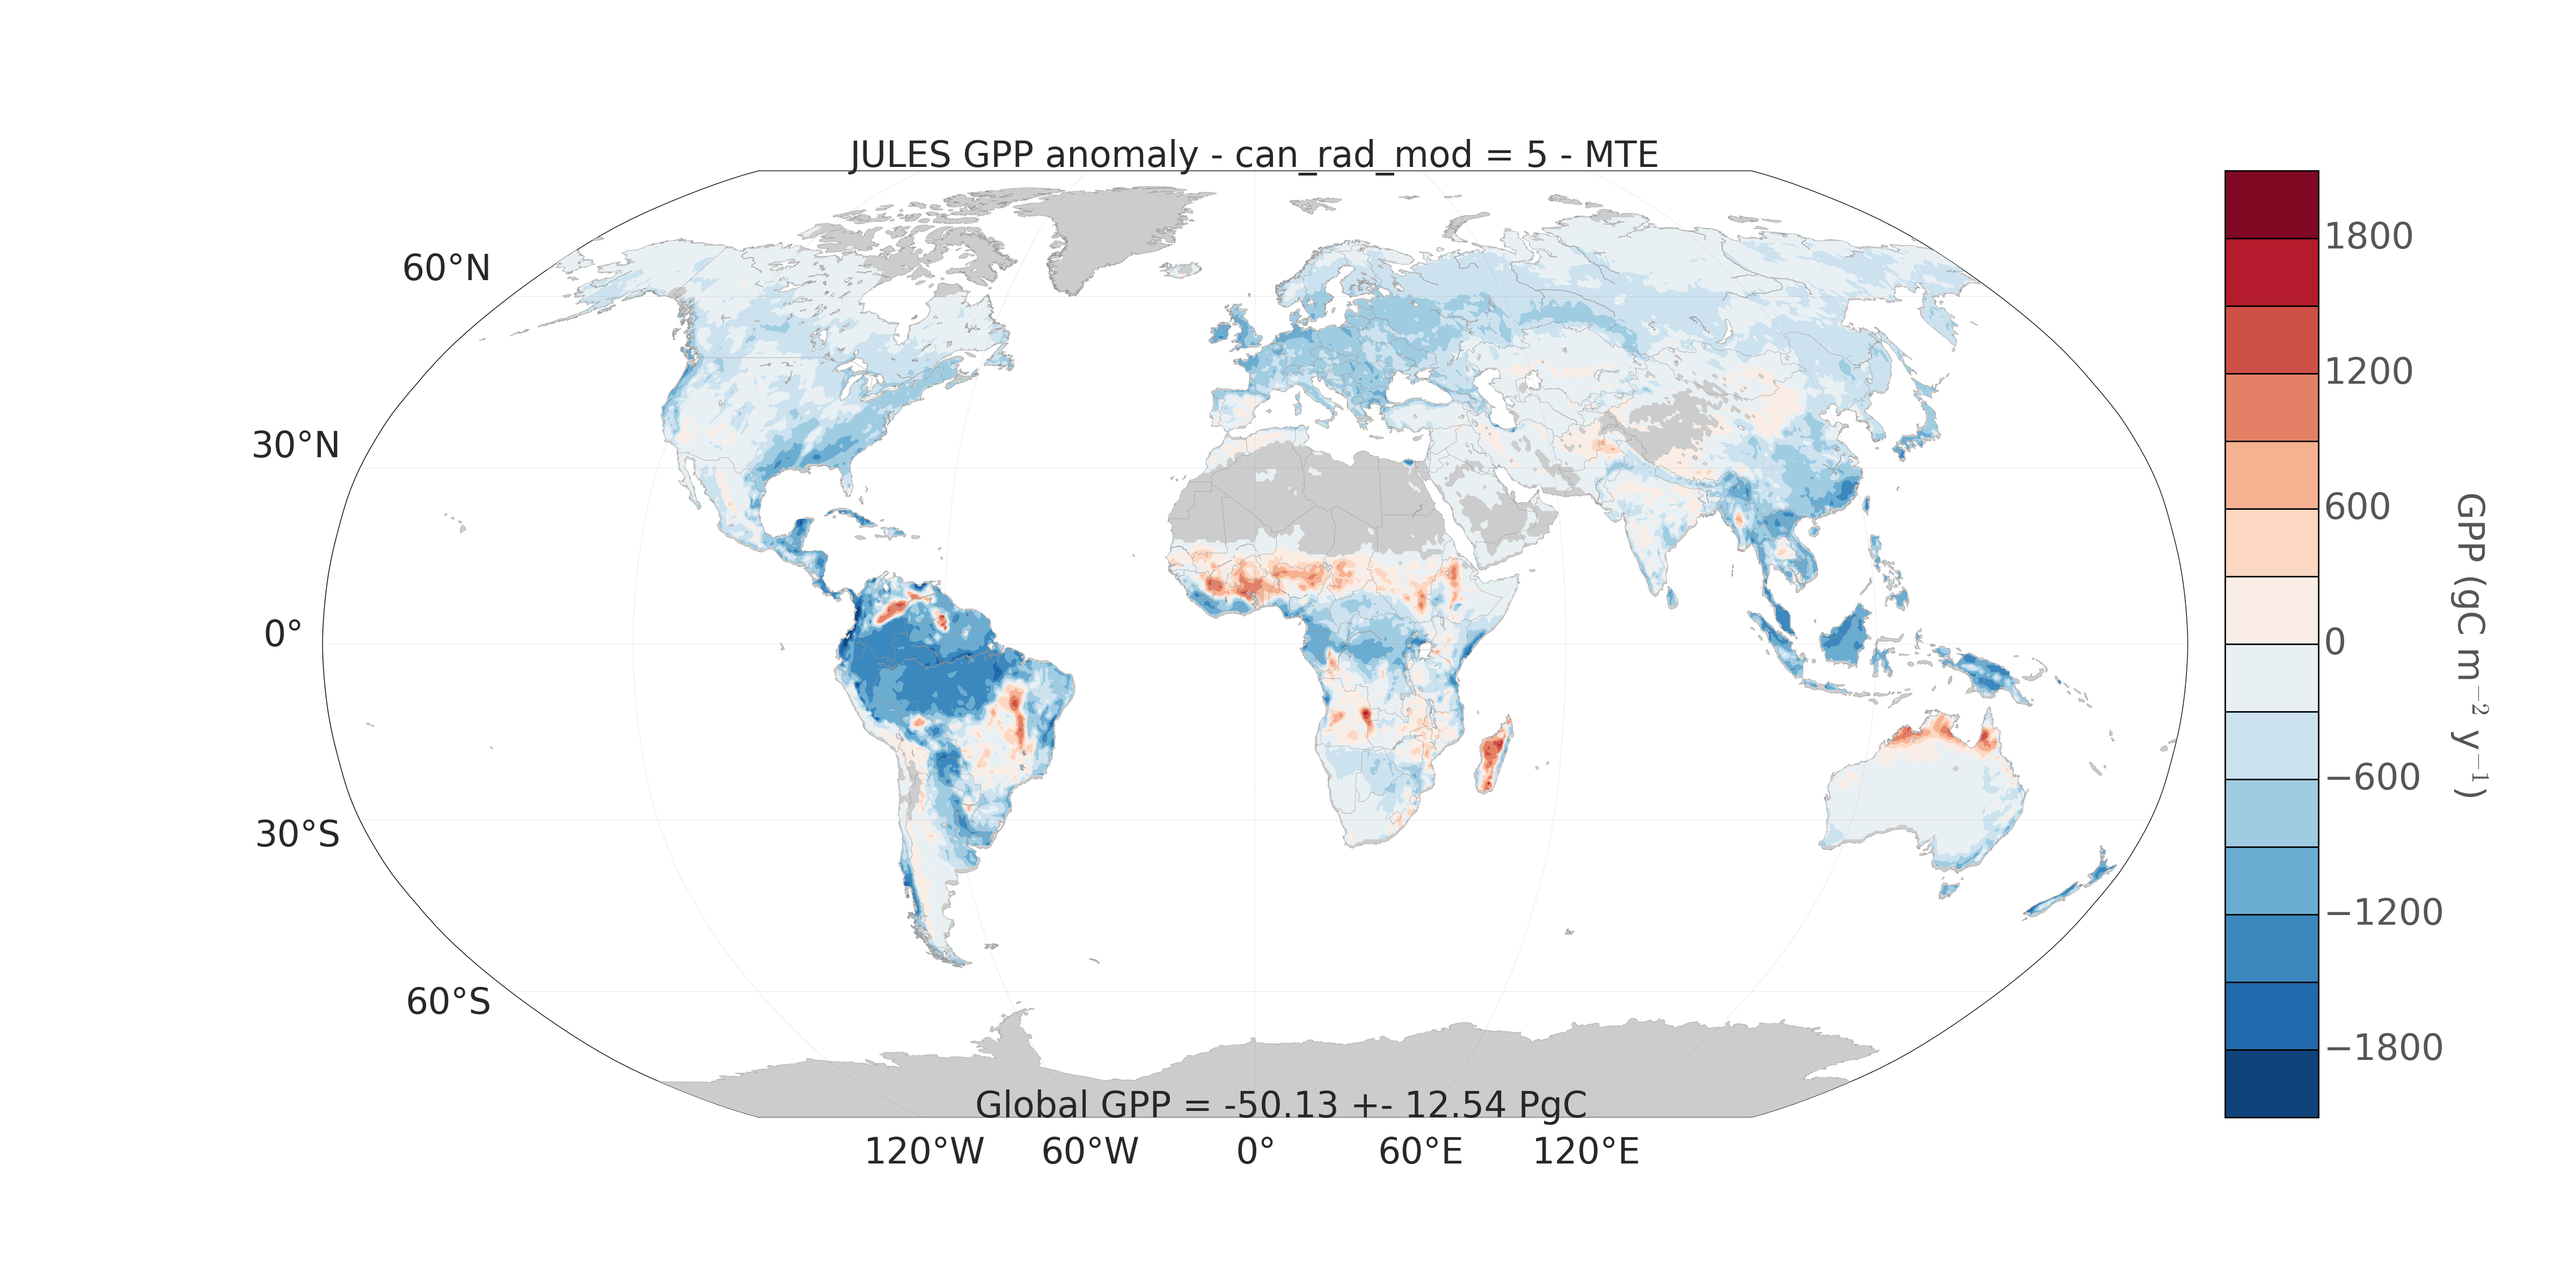
\includegraphics[width=0.5\textwidth]{/home/mn811042/Thesis/chapter6/figures_ofi/jules_mte_anom_opt50_MR_year.png}}
\subfloat[Opt 5 clump - MTE]{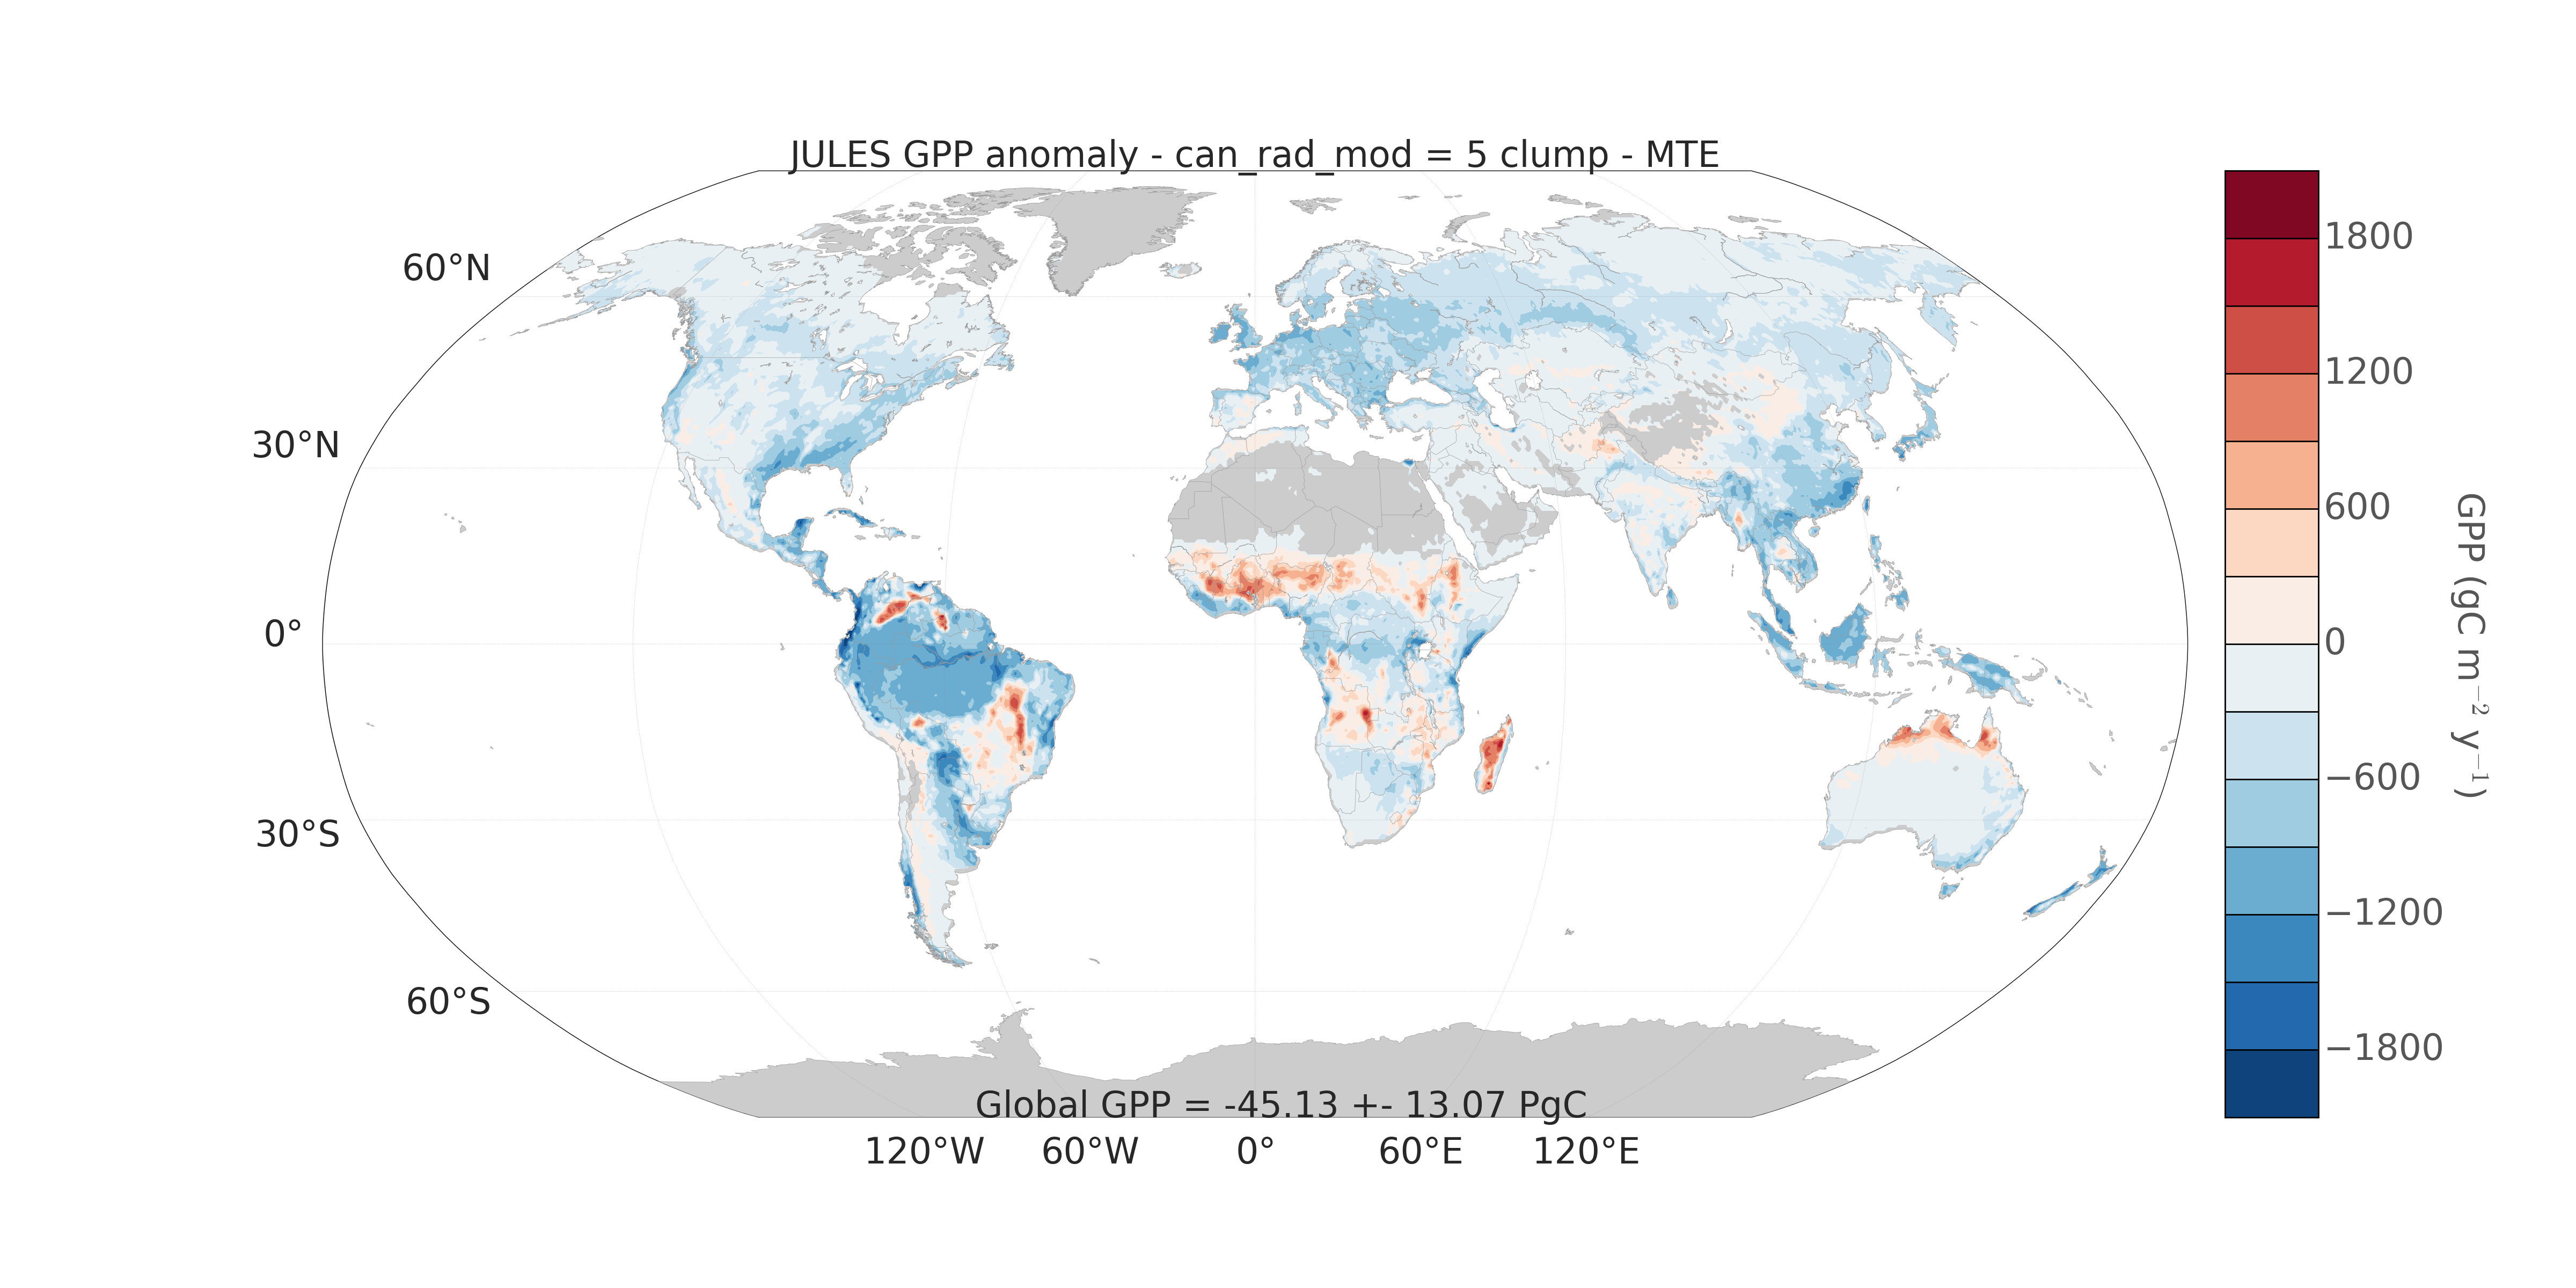
\includegraphics[width=0.5\textwidth]{/home/mn811042/Thesis/chapter6/figures_ofi/jules_mte_anom_opt50_clump_MR_year.png}}
\end{tabular}
\caption{Total average GPP for the year of 2008.} 
\label{f:pgap}
\end{figure}

\begin{figure}[ht!]
\centering
\begin{tabular}{ll}
\subfloat[Opt 4 - MTE]{\includegraphics[width=0.5\textwidth]{/home/mn811042/Thesis/chapter6/figures_ofi/adjust_4_mte_filtered_2.png}}
\subfloat[Opt 4 clump - MTE]{\includegraphics[width=0.5\textwidth]{/home/mn811042/Thesis/chapter6/figures_ofi/adjust_4_clump_mte_filtered_2.png}}
\end{tabular}
\begin{tabular}{ll}
\subfloat[Opt 4 - BL]{\includegraphics[width=0.5\textwidth]{/home/mn811042/Thesis/chapter6/figures_ofi/adjust_opt4_pft_0_filtered_3.png}}
\subfloat[Opt 4 clump - BL]{\includegraphics[width=0.5\textwidth]{/home/mn811042/Thesis/chapter6/figures_ofi/adjust_opt4_clump_pft_0_filtered_3.png}}
\end{tabular}
\begin{tabular}{ll}
\subfloat[Opt 4 - NL]{\includegraphics[width=0.5\textwidth]{/home/mn811042/Thesis/chapter6/figures_ofi/adjust_opt4_pft_1_filtered_3.png}}
\subfloat[Opt 4 clump - NL]{\includegraphics[width=0.5\textwidth]{/home/mn811042/Thesis/chapter6/figures_ofi/adjust_opt4_clump_pft_1_filtered_3.png}}
\end{tabular}
\caption{Comparison of JULES GPP through option 5 and the version with structure versus MTE applied only where the fraction of each gridbox is higher than 90\%  for the year of 2008.} 
\label{f:pgap}
\end{figure}


\begin{figure}[ht!]
\centering
\begin{tabular}{ll}
\subfloat[Opt 4 - C3]{\includegraphics[width=0.5\textwidth]{/home/mn811042/Thesis/chapter6/figures_ofi/adjust_opt4_pft_2_filtered_3.png}}
\subfloat[Opt 4 clump - C3]{\includegraphics[width=0.5\textwidth]{/home/mn811042/Thesis/chapter6/figures_ofi/adjust_opt4_clump_pft_2_filtered_3.png}}
\end{tabular}
\begin{tabular}{ll}
\subfloat[Opt 4 - C4]{\includegraphics[width=0.5\textwidth]{/home/mn811042/Thesis/chapter6/figures_ofi/adjust_opt4_pft_3_filtered_3.png}}
\subfloat[Opt 4 clump - C4]{\includegraphics[width=0.5\textwidth]{/home/mn811042/Thesis/chapter6/figures_ofi/adjust_opt4_clump_pft_3_filtered_3.png}}
\end{tabular}
\begin{tabular}{ll}
\subfloat[Opt 4 - SH]{\includegraphics[width=0.5\textwidth]{/home/mn811042/Thesis/chapter6/figures_ofi/adjust_opt4_pft_4_filtered_3.png}}
\subfloat[Opt 4 clump - SH]{\includegraphics[width=0.5\textwidth]{/home/mn811042/Thesis/chapter6/figures_ofi/adjust_opt4_clump_pft_4_filtered_3.png}}
\end{tabular}
\caption{Comparison of JULES GPP through option 5 and the version with structure versus MTE applied only where the fraction of each gridbox is higher than 90\%  for the year of 2008.} 
\label{f:pgap}
\end{figure}

\begin{figure}[ht!]
\centering
\begin{tabular}{ll}
\subfloat[Opt 5 - MTE]{\includegraphics[width=0.5\textwidth]{/home/mn811042/Thesis/chapter6/figures_ofi/adjust_5_mte_filtered_2.png}}
\subfloat[Opt 5 clump - MTE]{\includegraphics[width=0.5\textwidth]{/home/mn811042/Thesis/chapter6/figures_ofi/adjust_5_clump_mte_filtered_2.png}}
\end{tabular}
\begin{tabular}{ll}
\subfloat[Opt 5 - BL]{\includegraphics[width=0.5\textwidth]{/home/mn811042/Thesis/chapter6/figures_ofi/adjust_opt5_pft_0_filtered_3.png}}
\subfloat[Opt 5 clump - BL]{\includegraphics[width=0.5\textwidth]{/home/mn811042/Thesis/chapter6/figures_ofi/adjust_opt5_clump_pft_0_filtered_3.png}}
\end{tabular}
\begin{tabular}{ll}
\subfloat[Opt 5 - NL]{\includegraphics[width=0.5\textwidth]{/home/mn811042/Thesis/chapter6/figures_ofi/adjust_opt5_pft_1_filtered_3.png}}
\subfloat[Opt 5 clump - NL]{\includegraphics[width=0.5\textwidth]{/home/mn811042/Thesis/chapter6/figures_ofi/adjust_opt5_clump_pft_1_filtered_3.png}}
\end{tabular}
\caption{Comparison of JULES GPP through option 5 and the version with structure versus MTE applied only where the fraction of each gridbox is higher than 90\% for the year of 2008.} 
\label{f:pgap}
\end{figure}


\begin{figure}[ht!]
\centering
\begin{tabular}{ll}
\subfloat[Opt 5 - C3]{\includegraphics[width=0.5\textwidth]{/home/mn811042/Thesis/chapter6/figures_ofi/adjust_opt5_pft_2_filtered_3.png}}
\subfloat[Opt 5 clump - C3]{\includegraphics[width=0.5\textwidth]{/home/mn811042/Thesis/chapter6/figures_ofi/adjust_opt5_clump_pft_2_filtered_3.png}}
\end{tabular}
\begin{tabular}{ll}
\subfloat[Opt 5 - C4]{\includegraphics[width=0.5\textwidth]{/home/mn811042/Thesis/chapter6/figures_ofi/adjust_opt5_pft_3_filtered_3.png}}
\subfloat[Opt 5 clump - C4]{\includegraphics[width=0.5\textwidth]{/home/mn811042/Thesis/chapter6/figures_ofi/adjust_opt5_clump_pft_3_filtered_3.png}}
\end{tabular}
\begin{tabular}{ll}
\subfloat[Opt 5 - SH]{\includegraphics[width=0.5\textwidth]{/home/mn811042/Thesis/chapter6/figures_ofi/adjust_opt5_pft_4_filtered_3.png}}
\subfloat[Opt 5 clump - SH]{\includegraphics[width=0.5\textwidth]{/home/mn811042/Thesis/chapter6/figures_ofi/adjust_opt5_clump_pft_4_filtered_3.png}}
\end{tabular}
\caption{Comparison of JULES GPP through option 5 and the version with structure versus MTE applied only where the fraction of each gridbox is higher than 90\%  for the year of 2008.} 
\label{f:pgap}
\end{figure}

These numbers where obtained by divinding the number of gridbox in each limiting regime by the total amount of pixels in land. Option 5 has 6 gridbox more than Option 4, i.e., 57128 vs. 57122. The percentual distribution of limiting regimes is not affected by the canopy radiation mode used in JULES, and the impact of structure is roughly the same between both canopy radiation modes. 

Option 5: Light = 52.2\%, Carbon = 43.3\%, Export = 4.5\%

Option 5 clump: Light = 42.9\%, Carbon = 51.5\%, Export = 5.6\%

Difference: Light = -9.3\%, Carbon = 8.2\%, Export = 1.1\%

\begin{figure}[ht!]
\centering\hspace*{-1.9in}
\begin{tabular}{ll}
\subfloat[Diff Opt 4 clump - 4]{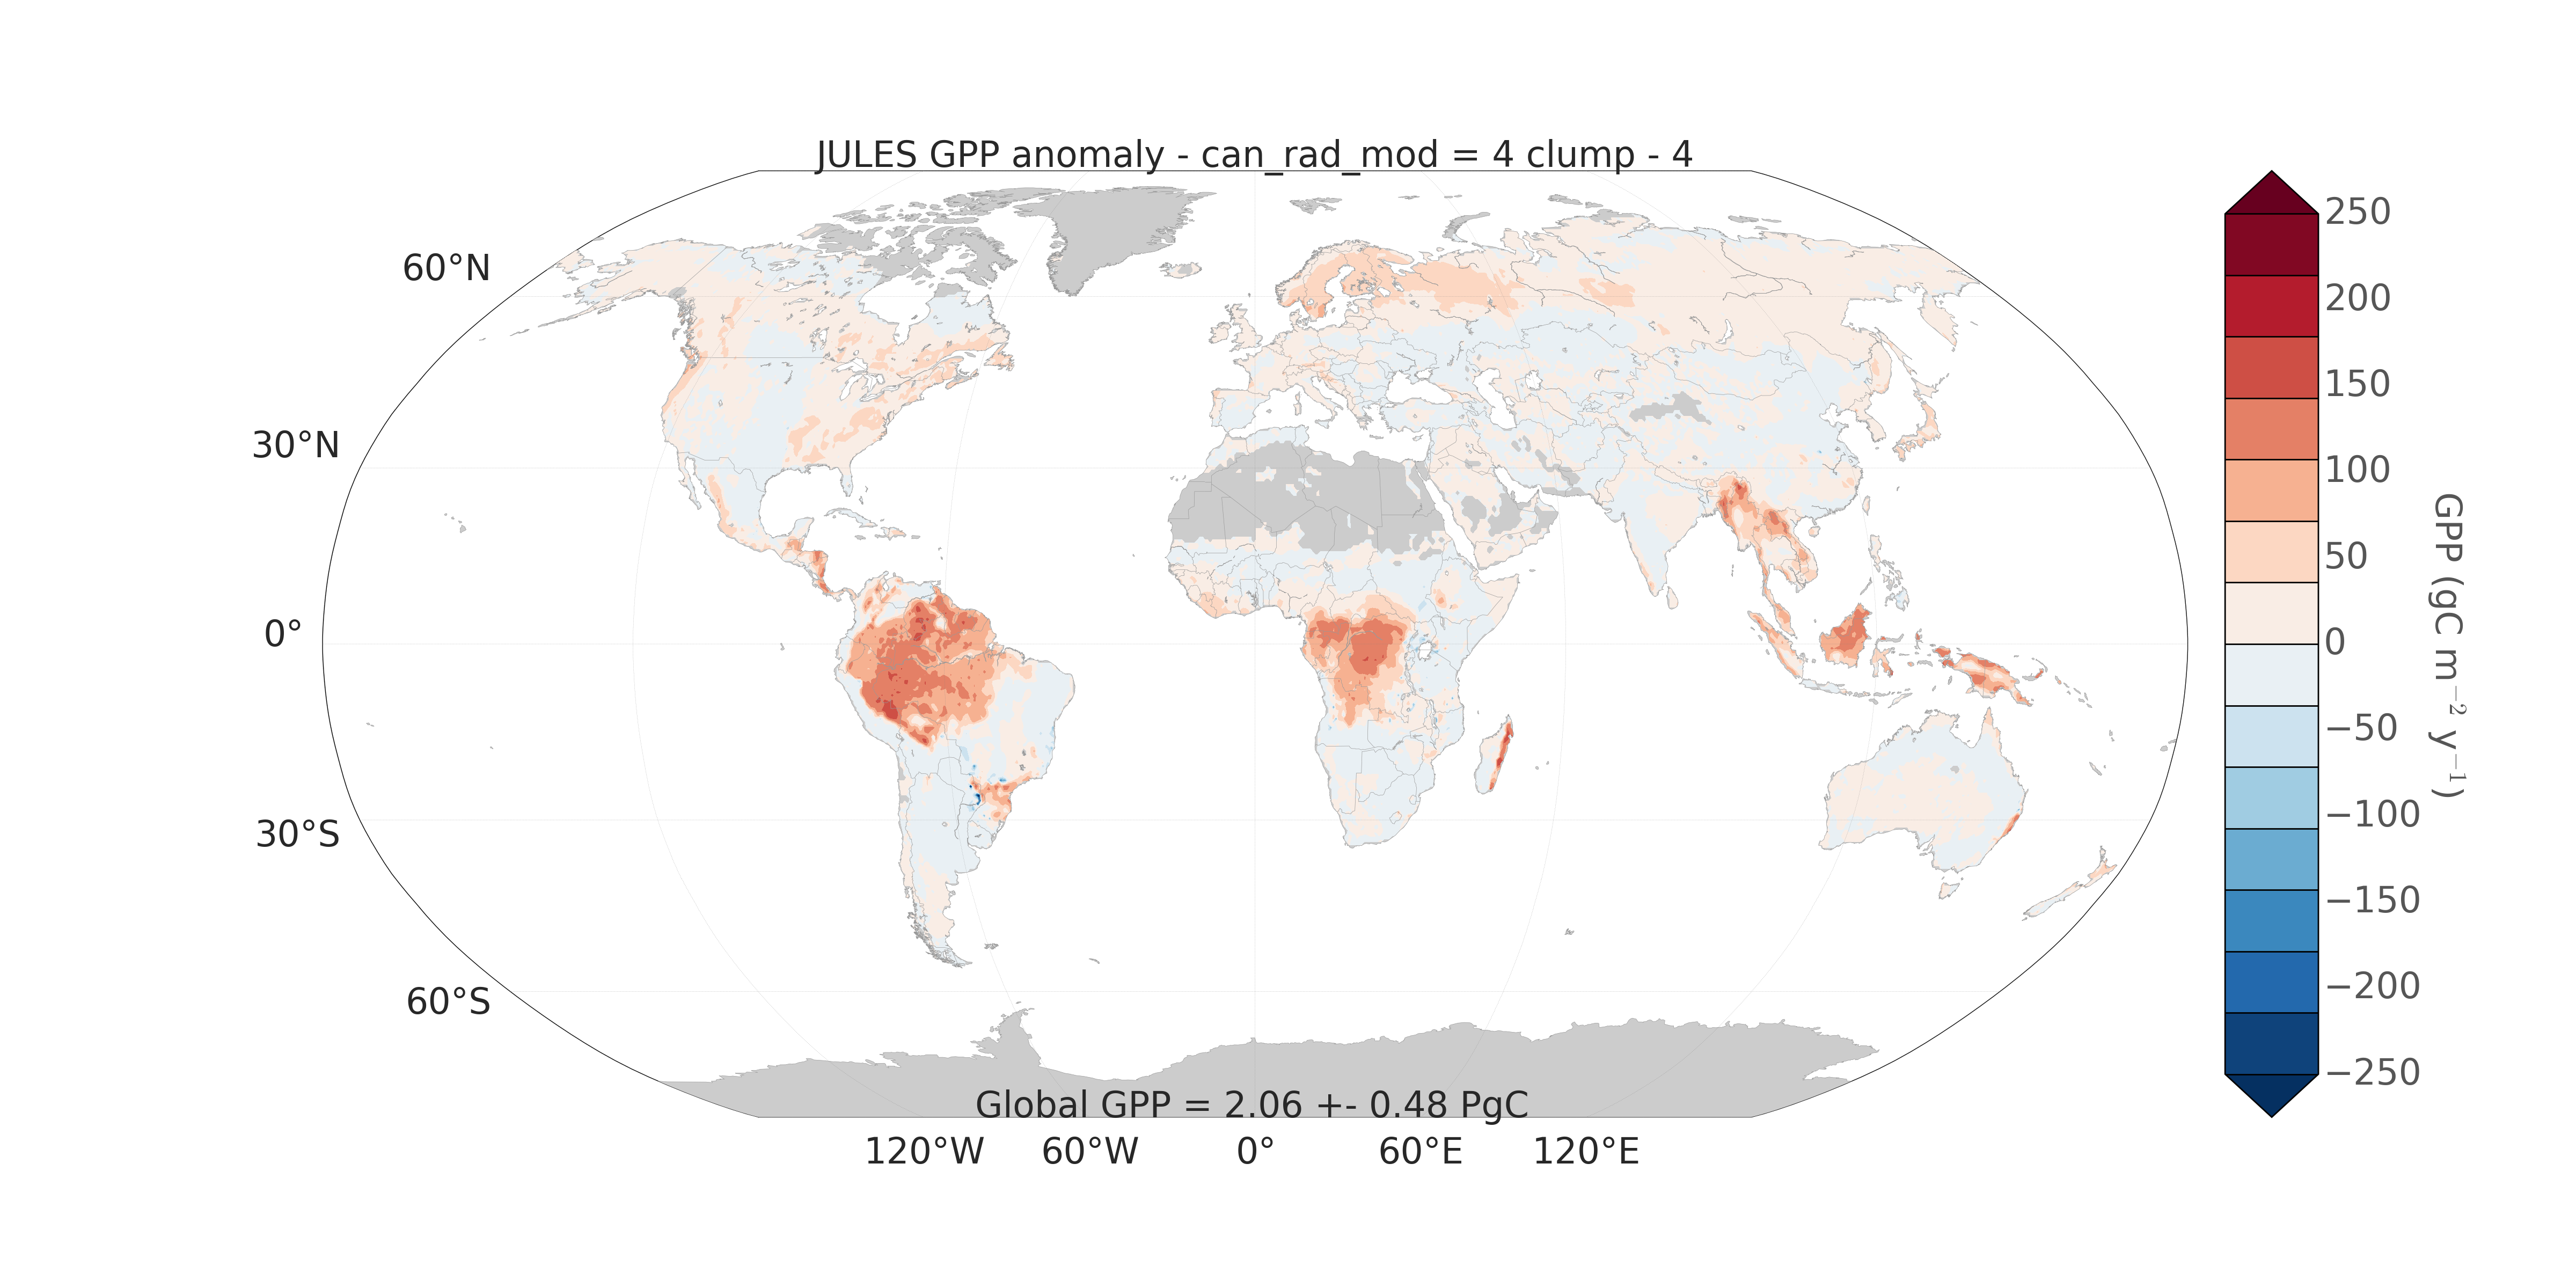
\includegraphics[width=0.7\textwidth]{/home/mn811042/Thesis/chapter6/figures_ofi/jules_anom_opt4_clump_MR_year.png}}
\subfloat[Diff Opt 5 clump - 5]{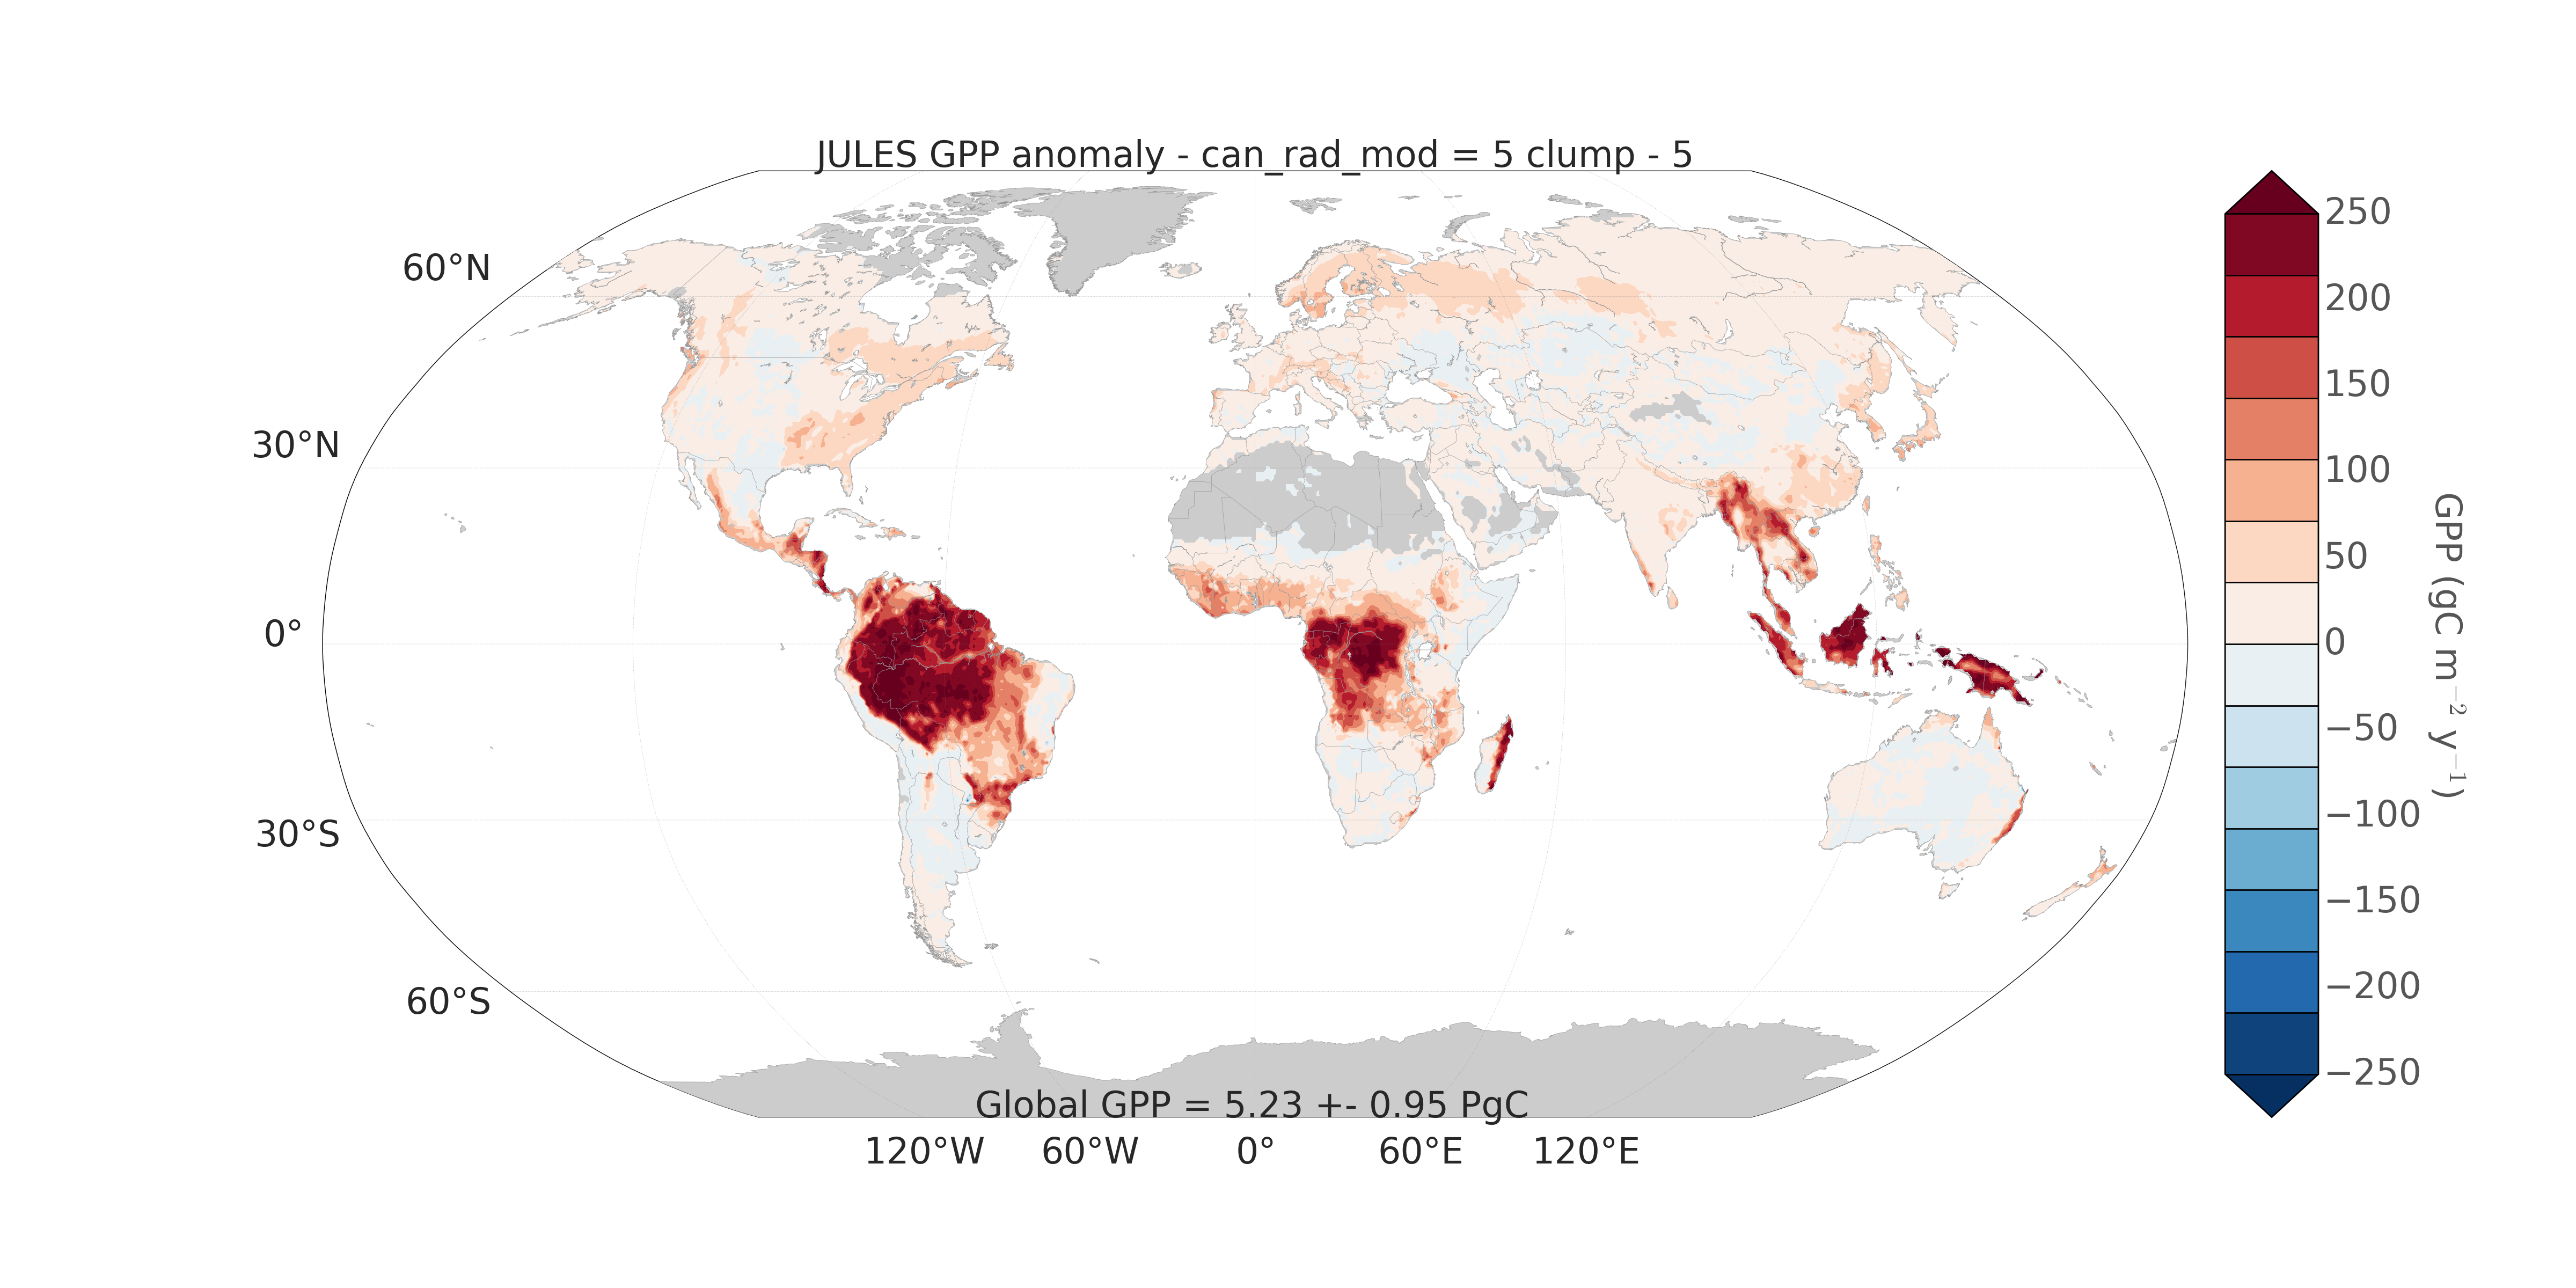
\includegraphics[width=0.7\textwidth]{/home/mn811042/Thesis/chapter6/figures_ofi/jules_anom_opt5_clump_MR_year.png}}
\end{tabular}
\centering\hspace*{-1.9in}
\begin{tabular}{ll}
\subfloat[Opt 4 BL]{\includegraphics[width=0.7\textwidth]{/home/mn811042/Thesis/chapter6/figures_ofi/jules_anom_opt4_pft_0_clump_MR_year.png}}
\subfloat[Opt 5 BL]{\includegraphics[width=0.7\textwidth]{/home/mn811042/Thesis/chapter6/figures_ofi/jules_anom_opt5_pft_0_clump_MR_year.png}}
\end{tabular}
\centering\hspace*{-1.9in}
\begin{tabular}{ll}
\subfloat[Opt 4 NL]{\includegraphics[width=0.7\textwidth]{/home/mn811042/Thesis/chapter6/figures_ofi/jules_anom_opt4_pft_1_clump_MR_year.png}}
\subfloat[Opt 5 NL]{\includegraphics[width=0.7\textwidth]{/home/mn811042/Thesis/chapter6/figures_ofi/jules_anom_opt5_pft_1_clump_MR_year.png}}
\end{tabular}

\caption{Spatial impact of clumping per PFT for two radiative transfer modules in JULES.} 
\label{f:pgap}
\end{figure}


\begin{figure}[ht!]
\centering\hspace*{-1.9in}
\begin{tabular}{ll}
\subfloat[Opt 4 C3]{\includegraphics[width=0.7\textwidth]{/home/mn811042/Thesis/chapter6/figures_ofi/jules_anom_opt4_pft_2_clump_MR_year.png}}
\subfloat[Opt 5 C3]{\includegraphics[width=0.7\textwidth]{/home/mn811042/Thesis/chapter6/figures_ofi/jules_anom_opt5_pft_2_clump_MR_year.png}}
\end{tabular}
\centering\hspace*{-1.9in}
\begin{tabular}{ll}
\subfloat[Opt 4 C4]{\includegraphics[width=0.7\textwidth]{/home/mn811042/Thesis/chapter6/figures_ofi/jules_anom_opt4_pft_3_clump_MR_year.png}}
\subfloat[Opt 5 C4]{\includegraphics[width=0.7\textwidth]{/home/mn811042/Thesis/chapter6/figures_ofi/jules_anom_opt5_pft_3_clump_MR_year.png}}
\end{tabular}
\centering\hspace*{-1.9in}
\begin{tabular}{ll}
\subfloat[Opt 4 SH]{\includegraphics[width=0.7\textwidth]{/home/mn811042/Thesis/chapter6/figures_ofi/jules_anom_opt4_pft_4_clump_MR_year.png}}
\subfloat[Opt 5 SH]{\includegraphics[width=0.7\textwidth]{/home/mn811042/Thesis/chapter6/figures_ofi/jules_anom_opt5_pft_4_clump_MR_year.png}}
\end{tabular}
\caption{Spatial impact of clumping on absolute GPP per PFT for two radiative transfer modules in JULES.} 
\label{f:pgap}
\end{figure}

\begin{figure}[ht!]
\centering\hspace*{-1.9in}
\begin{tabular}{ll}
\subfloat[Diff Opt 4 clump - 4]{\includegraphics[width=0.7\textwidth]{/home/mn811042/Thesis/chapter6/figures_ofi/jules_perc_anom_opt4_clump_MR_year.png}}
\subfloat[Diff Opt 5 clump - 5]{\includegraphics[width=0.7\textwidth]{/home/mn811042/Thesis/chapter6/figures_ofi/jules_perc_anom_opt5_clump_MR_year.png}}
\end{tabular}
\centering\hspace*{-1.9in}
\begin{tabular}{ll}
\subfloat[Opt 4 BL]{\includegraphics[width=0.7\textwidth]{/home/mn811042/Thesis/chapter6/figures_ofi/jules_perc_anom_opt4_pft_0_clump_MR_year.png}}
\subfloat[Opt 5 BL]{\includegraphics[width=0.7\textwidth]{/home/mn811042/Thesis/chapter6/figures_ofi/jules_perc_anom_opt5_pft_0_clump_MR_year.png}}
\end{tabular}
\centering\hspace*{-1.9in}
\begin{tabular}{ll}
\subfloat[Opt 4 NL]{\includegraphics[width=0.7\textwidth]{/home/mn811042/Thesis/chapter6/figures_ofi/jules_perc_anom_opt4_pft_1_clump_MR_year.png}}
\subfloat[Opt 5 NL]{\includegraphics[width=0.7\textwidth]{/home/mn811042/Thesis/chapter6/figures_ofi/jules_perc_anom_opt5_pft_1_clump_MR_year.png}}
\end{tabular}

\caption{Spatial impact of clumping per PFT for two radiative transfer modules in JULES.} 
\label{f:pgap}
\end{figure}


\begin{figure}[ht!]
\centering\hspace*{-1.9in}
\begin{tabular}{ll}
\subfloat[Opt 4 C3]{\includegraphics[width=0.7\textwidth]{/home/mn811042/Thesis/chapter6/figures_ofi/jules_perc_anom_opt4_pft_2_clump_MR_year.png}}
\subfloat[Opt 5 C3]{\includegraphics[width=0.7\textwidth]{/home/mn811042/Thesis/chapter6/figures_ofi/jules_perc_anom_opt5_pft_2_clump_MR_year.png}}
\end{tabular}
\centering\hspace*{-1.9in}
\begin{tabular}{ll}
\subfloat[Opt 4 C4]{\includegraphics[width=0.7\textwidth]{/home/mn811042/Thesis/chapter6/figures_ofi/jules_perc_anom_opt4_pft_3_clump_MR_year.png}}
\subfloat[Opt 5 C4]{\includegraphics[width=0.7\textwidth]{/home/mn811042/Thesis/chapter6/figures_ofi/jules_perc_anom_opt5_pft_3_clump_MR_year.png}}
\end{tabular}
\centering\hspace*{-1.9in}
\begin{tabular}{ll}
\subfloat[Opt 4 SH]{\includegraphics[width=0.7\textwidth]{/home/mn811042/Thesis/chapter6/figures_ofi/jules_perc_anom_opt4_pft_4_clump_MR_year.png}}
\subfloat[Opt 5 SH]{\includegraphics[width=0.7\textwidth]{/home/mn811042/Thesis/chapter6/figures_ofi/jules_perc_anom_opt5_pft_4_clump_MR_year.png}}
\end{tabular}
\caption{Spatial impact of clumping on relative GPP per PFT for two radiative transfer modules in JULES.} 
\label{f:pgap}
\end{figure}


\newpage
\pagestyle{plain}
\bibliographystyle{/home/mn811042/Thesis/format_files/ametsoc}
\bibliography{/home/mn811042/Thesis/chapter6/ch6_v1}
%\bibliography{../bib_docs/library_15_7_2016}
%\bibliography{../bib_docs/library_24_3_2016}
%\bibliographystyle{abbrvnat}   % initials

%\begin{appendices}
%\normalsize
%\chapter{fAPAR vertical distribution}\label{appendix:a}



%\end{appendices}

\end{document}
